\documentclass[11pt,twoside]{book}

%% include commands for bios, titles etc used in multiple documents
% $Date$
% $Revision$
% $Author$

%%%%%%%%%%%%%%%%%%%%%%%%%%%%%%%%%%%%%%%%%%%%%%%%%%%%%%%%%%%%%%%%%%%%%%%%%%%%%%%%%%%%%%%%%%%%%%%%%%%
%                                                                                                 %
% The mathematical style of these documents follows                                               %
%                                                                                                 %
% A. Thompson and B.N. Taylor. The NIST Guide for the Use of the International System of Units.   %
%    NIST Special Publication 881, 2008.                                                          %
%                                                                                                 %
% http://www.nist.gov/pml/pubs/sp811/index.cfm                                                    %
%                                                                                                 %
%%%%%%%%%%%%%%%%%%%%%%%%%%%%%%%%%%%%%%%%%%%%%%%%%%%%%%%%%%%%%%%%%%%%%%%%%%%%%%%%%%%%%%%%%%%%%%%%%%%

% Packages which force the use of better TeX coding
% Mostly from http://tex.stackexchange.com/q/19264
%%\RequirePackage[l2tabu, orthodox]{nag}
%%\usepackage{fixltx2e}
%\usepackage{isomath} % Disabled for the moment because it changes the syntax for bold and roman Greek math symbols
%%\usepackage[all,warning]{onlyamsmath}
%\usepackage{strict} % Commented out for now because it is uncommon. A copy of style.sty is in Manuals/LaTeX_Style_Files/.

\usepackage{times,mathptmx}
\usepackage[pdftex]{graphicx}
\usepackage{tabularx}
\usepackage{multirow}
\usepackage{pdfsync}
\usepackage{tikz}
\usepackage{pgfplots}
%\pgfplotsset{compat=1.7}
\usepackage{tocloft}
\usepackage{color}
\usepackage{amsmath}
\definecolor{linknavy}{rgb}{0,0,0.50196}
\definecolor{linkred}{rgb}{1,0,0}
\definecolor{linkblue}{rgb}{0,0,1}
\usepackage{float}
\usepackage{caption}
\usepackage{graphpap}
\usepackage{rotating}
\usepackage{geometry}
\usepackage{relsize}
\usepackage{longtable}
\usepackage{lscape}
\usepackage{amssymb}
\usepackage{makeidx} % Create index at end of document
\usepackage[nottoc,notlof,notlot]{tocbibind} % Put the bibliography and index in the ToC
\usepackage{lastpage} % Automatic last page number reference.
\usepackage[T1]{fontenc}
\usepackage{enumerate}
\usepackage{upquote}
\usepackage{moreverb}
\usepackage{morefloats}

% Smokeview Version String
\newcommand{\smvversion}{6.5.0}

\newcommand{\nopart}{\expandafter\def\csname Parent-1\endcsname{}} % To fix table of contents in pdf.
\newcommand{\ct}{\tt\small} % eventually will be deprecated due to http://www.tex.ac.uk/cgi-bin/texfaq2html?label=2letterfontcmd
\newcommand{\textct}[1]{\texttt{\small #1}}

\usepackage{tocstyle} % Fix table of contents sections from overlapping section titles
\usetocstyle{standard}
\usepackage{siunitx}
\sisetup{
    detect-all = true,
    input-decimal-markers = {.},
    input-ignore = {,},
    inter-unit-product = \ensuremath{{}\cdot{}},
    multi-part-units = repeat,
    number-unit-product = \text{~},
    per-mode = fraction,
    separate-uncertainty = true,
}

\usepackage{listings}
\usepackage{textcomp}
\definecolor{lbcolor}{rgb}{0.96,0.96,0.96}
\lstset{
    %backgroundcolor=\color{lbcolor},
    tabsize=4,
    rulecolor=,
    language=Fortran,
        basicstyle=\footnotesize\ttfamily,
        upquote=true,
        aboveskip={\baselineskip},
        belowskip={\baselineskip},
        columns=fixed,
        extendedchars=true,
        breaklines=true,
        breakatwhitespace=true,
        frame=none,
        showtabs=false,
        showspaces=false,
        showstringspaces=false,
        identifierstyle=\ttfamily,
        keywordstyle=\color[rgb]{0,0,0},
        commentstyle=\color[rgb]{0,0,0},
        stringstyle=\color[rgb]{0,0,0},
}

\usepackage{xr-hyper}
\usepackage[pdftex,
        colorlinks=true,
        urlcolor=linkblue,     % \href{...}{...} external (URL)
        citecolor=linkred,     % citation number colors
        linkcolor=linknavy,    % \ref{...} and \pageref{...}
        pdfproducer={pdflatex},
        pagebackref,
        pdfpagemode=UseNone,
        bookmarksopen=true,
        plainpages=false,
        verbose]{hyperref}

% The Following commented code makes the ``Draft'' watermark on each page.
%\usepackage{eso-pic}
%\usepackage{type1cm}
%\makeatletter
%   \AddToShipoutPicture{
%     \setlength{\@tempdimb}{.5\paperwidth}
%     \setlength{\@tempdimc}{.5\paperheight}
%     \setlength{\unitlength}{1pt}
%     \put(\strip@pt\@tempdimb,\strip@pt\@tempdimc){
%     \makebox(0,0){\rotatebox{45}{\textcolor[gray]{0.75}{\fontsize{8cm}\selectfont{RC6}}}}}
% }
%\makeatother

\setlength{\textwidth}{6.5in}
\setlength{\textheight}{9.0in}
\setlength{\topmargin}{0.in}
\setlength{\headheight}{0.in}
\setlength{\headsep}{0.in}
\setlength{\parindent}{0.25in}
\setlength{\oddsidemargin}{0.0in}
\setlength{\evensidemargin}{0.0in}
\setlength{\leftmargini}{\parindent} % Controls the indenting of the "bullets" in a list
\setlength{\cftsecnumwidth}{0.45in}
\setlength{\cftsubsecnumwidth}{0.5in}
\setlength{\cftfignumwidth}{0.45in}
\setlength{\cfttabnumwidth}{0.45in}

\newcommand{\authortitlesigs}
{
\begin{flushright}
Kevin McGrattan \\
Simo Hostikka \\
Randall McDermott \\
Jason Floyd \\
Craig Weinschenk \\
Kristopher Overholt
\end{flushright}
}

\newcommand{\logosigs}{
\begin{minipage}[b]{6.5in}
\parbox[b]{3.5in}{

\includegraphics[width=1.3in]{../Bibliography/VTT_BLACK_L} \\
VTT Technical Research Centre of Finland}
\hfill
\parbox[b]{3in}{\flushright{
\includegraphics[width=2.in]{../Bibliography/nistident_flright_vec}}}
\end{minipage}
}

\newcommand{\authorsigs}
{
\begin{flushright}
Kevin McGrattan \\
Randall McDermott \\
{\em Fire Research Division \\
Engineering Laboratory \\
Gaithersburg, Maryland, USA} \\[.1in]
Simo Hostikka \\
{\em Aalto University \\
Espoo, Finland} \\[.1in]
Jason Floyd \\
Craig Weinschenk \\
{\em Jensen Hughes \\
Baltimore, Maryland, USA}\\[.1in]
Kristopher Overholt \\
{\em Continuum Analytics \\
Austin, Texas, USA}
\end{flushright}
}

\newcommand{\titlesigs}
{
\small
\begin{flushright}
U.S. Department of Commerce \\
{\em Wilbur L. Ross, Jr., Secretary} \\
\hspace{1in} \\
National Institute of Standards and Technology \\
{\em Kent Rochford, Acting Under Secretary of Commerce for Standards and Technology and Acting NIST Director}
\end{flushright}
}


\newcommand{\disclaimer}[1]{
\begin{minipage}[t][8in][s]{6.5in}
\fontsize{10}{12}\selectfont
\flushright{Certain commercial entities, equipment, or materials may be identified in this \\
document in order to describe an experimental procedure or concept adequately. \\
Such identification is not intended to imply recommendation or endorsement by the \\
National Institute of Standards and Technology, nor is it intended to imply that the \\
entities, materials, or equipment are necessarily the best available for the purpose.\\
}

\vspace{3in}

\large
\flushright{\bf National Institute of Standards and Technology Special Publication #1 \\
Natl.~Inst.~Stand.~Technol.~Spec.~Publ.~#1, \pageref{LastPage} pages (October 2013) \\
CODEN: NSPUE2 }

\vfill

\hspace{1in}

\end{minipage}
}



\newcommand{\gforneybio}
{
\item[Glenn Forney] is a computer scientist at the Engineering Laboratory of NIST.  He received a
bachelor of science degree in mathematics from Salisbury State College and a master of
science and a doctorate in mathematics from Clemson University.  He joined NIST
in 1986 (then the National Bureau of Standards) and has since worked on developing tools that
provide a better understanding of fire phenomena, most notably Smokeview, a software tool for visualizing
Fire Dynamics Simulator data.
}

\newcommand{\smvoverview}
{
This guide is part of a three volume set of companion documents describing how to use Smokeview
in Volume I, the Smokeview User's Guide~\cite{Smokeview_Users_Guide}, describing technical details of how the visualizations are performed in Volume II, the Smokeview Technical Reference Guide~\cite{Smokeview_Tech_Guide}, and presents example cases
verifying the various visualization capabilities of Smokeview in Volume III, the Smokeview Verification Guide~\cite{Smokeview_Verification_Guide}.  Details on the use and technical background of the Fire Dynamics Simulator is contained in the FDS User's~\cite{FDS_Users_Guide} and Technical reference guide~\cite{FDS_Math_Guide}
respectively.
}

% commands to use for "official" cover and title pages
% see smokeview verification guide to see how they are used

\newcommand{\headerA}[1]{
\begin{flushright}
\fontsize{20}{24}\selectfont
\bf{NIST Special Publication #1}
\end{flushright}
}


\newcommand{\headerB}[1]{
\begin{flushright}
\fontsize{28}{33.6}\selectfont
\bf{#1}
\end{flushright}
}

\newcommand{\headerC}[1]{
\vspace{.15in}
\begin{flushright}
\fontsize{12}{14}\selectfont
#1
\end{flushright}
}

\newcommand{\headerD}[1]{
\begin{flushright}
\fontsize{12}{14}\selectfont
http://dx.doi.org/10.6028/NIST.SP.#1
\end{flushright}
}



\newcommand{\dod}[2]{\frac{\partial #1}{\partial #2}}
\newcommand{\DoD}[2]{\frac{\mathrm{D} #1}{\mathrm{D} #2}}
\newcommand{\dsods}[2]{\frac{\partial^2 #1}{\partial #2^2}}
\renewcommand{\d}{\,\mathrm{d}}
\newcommand{\dx}{\delta x}
\newcommand{\dy}{\delta y}
\newcommand{\dz}{\delta z}
\newcommand{\degF}{$^\circ$F}
\newcommand{\degC}{$^\circ$C}
\newcommand{\x}{x}
\newcommand{\y}{y}
\newcommand{\z}{z}
\newcommand{\dt}{\delta t}
\newcommand{\dn}{\delta n}
\newcommand{\cH}{H}
\newcommand{\hu}{u}
\newcommand{\hv}{v}
\newcommand{\hw}{w}
\newcommand{\la}{\lambda}
\newcommand{\bO}{{\Omega}}
\newcommand{\bo}{{\mathbf{\omega}}}
\newcommand{\btau}{\mathbf{\tau}}
\newcommand{\bdelta}{{\mathbf{\delta}}}
\newcommand{\sumyw}{\sum (Y_\alpha/W_\alpha)}
\newcommand{\oW}{\overline{W}}
\newcommand{\om}{\ensuremath{\omega}}
\newcommand{\omx}{\omega_x}
\newcommand{\omy}{\omega_y}
\newcommand{\omz}{\omega_z}
\newcommand{\erf}{\hbox{erf}}
\newcommand{\erfc}{\hbox{erfc}}
\newcommand{\bF}{{\mathbf{F}}}
\newcommand{\bG}{{\mathbf{G}}}
\newcommand{\bof}{{\mathbf{f}}}
\newcommand{\bq}{{\mathbf{q}}}
\newcommand{\br}{{\mathbf{r}}}
\newcommand{\bu}{{\mathbf{u}}}
\newcommand{\bx}{{\mathbf{x}}}
\newcommand{\bk}{{\mathbf{k}}}
\newcommand{\bv}{{\mathbf{v}}}
\newcommand{\bg}{{\mathbf{g}}}
\newcommand{\bn}{{\mathbf{n}}}
\newcommand{\bS}{{\mathbf{S}}}
\newcommand{\bW}{\overline{W}}
\newcommand{\dS}{d{\mathbf{S}}}
\newcommand{\bs}{{\mathbf{s}}}
\newcommand{\bI}{{\mathbf{I}}}
\newcommand{\hp}{H}
\newcommand{\trho}{\tilde{\rho}}
\newcommand{\dph}{{\delta\phi}}
\newcommand{\dth}{{\delta\theta}}
\newcommand{\tp}{\tilde{p}}
\newcommand{\bp}{\overline{p}}
\newcommand{\dQ}{\dot{Q}}
\newcommand{\dq}{\dot{q}}
\newcommand{\dbq}{\dot{\mathbf{q}}}
\newcommand{\dm}{\dot{m}}
\newcommand{\ha}{\frac{1}{2}}
\newcommand{\ft}{\frac{4}{3}}
\newcommand{\ot}{\frac{1}{3}}
\newcommand{\fofi}{\frac{4}{5}}
\newcommand{\of}{\frac{1}{4}}
\newcommand{\twth}{\frac{2}{3}}
\newcommand{\R}{R}
\newcommand{\be}{\begin{equation}}
\newcommand{\ee}{\end{equation}}
\newcommand{\RE}{\hbox{Re}}
\newcommand{\LE}{\hbox{Le}}
\newcommand{\PR}{\hbox{Pr}}
\newcommand{\PE}{\hbox{Pe}}
\newcommand{\NU}{\hbox{Nu}}
\newcommand{\SC}{\hbox{Sc}}
\newcommand{\SH}{\hbox{Sh}}
\newcommand{\WE}{\hbox{We}}
\newcommand{\COTWO}{\text{\tiny \hbox{CO}$_2$}}
\newcommand{\HTWOO}{\text{\tiny \hbox{H}$_2$\hbox{O}}}
\newcommand{\OTWO}{\text{\tiny \hbox{O}$_2$}}
\newcommand{\NTWO}{\text{\tiny \hbox{N}$_2$}}
\newcommand{\CO}{\text{\tiny \hbox{CO}}}
\newcommand{\F}{\text{\tiny \hbox{F}}}
\newcommand{\C}{\text{\tiny \hbox{C}}}
\newcommand{\Hy}{\text{\tiny \hbox{H}}}
\newcommand{\So}{\text{\tiny \hbox{S}}}
\newcommand{\M}{\text{\tiny \hbox{M}}}
\newcommand{\xx}{\text{\tiny \hbox{x}}}
\newcommand{\yy}{\text{\tiny \hbox{y}}}
\newcommand{\zz}{\text{\tiny \hbox{z}}}
\newcommand{\smvlines}{135~000}

\newcommand{\calH}{\mathcal{H}}
\newcommand{\calR}{\mathcal{R}}

\newcommand{\dif}{\mathrm{d}}
\newcommand{\Div}{\nabla\cdot}
\newcommand{\D}{\mbox{D}}
\newcommand{\mhalf}{\mbox{$\frac{1}{2}$}}
\newcommand{\thalf}{\mbox{\tiny $\frac{1}{2}$}}
\newcommand{\tripleprime}{{\prime\prime\prime}}
\newcommand{\ppp}{{\prime\prime\prime}}
\newcommand{\pp}{{\prime\prime}}

\newcommand{\superscript}[1]{\ensuremath{^{\textrm{\tiny #1}}}}
\newcommand{\subscript}[1]{\ensuremath{_{\textrm{\tiny #1}}}}

\newcommand{\rb}[1]{\raisebox{1.5ex}[0pt]{#1}}

\newcommand{\Ra}{$\Rightarrow$}
\newcommand{\hhref}[1]{\href{#1}{{\tt #1}}}
\newcommand{\fdsinput}[1]{{\scriptsize\verbatiminput{../../Verification/Visualization/#1}}}

\definecolor{AQUAMARINE}{rgb}{0.49804,1.00000,0.83137}
\definecolor{ANTIQUE WHITE}{rgb}{0.98039,0.92157,0.84314}
\definecolor{BEIGE}{rgb}{0.96078,0.96078,0.86275}
\definecolor{BLACK}{rgb}{0.00000,0.00000,0.00000}
\definecolor{BLUE}{rgb}{0.00000,0.00000,1.00000}
\definecolor{BLUE VIOLET}{rgb}{0.54118,0.16863,0.88627}
\definecolor{BRICK}{rgb}{0.61176,0.40000,0.12157}
\definecolor{BROWN}{rgb}{0.64706,0.16471,0.16471}
\definecolor{BURNT SIENNA}{rgb}{0.54118,0.21176,0.05882}
\definecolor{BURNT UMBER}{rgb}{0.54118,0.20000,0.14118}
\definecolor{CADET BLUE}{rgb}{0.37255,0.61961,0.62745}
\definecolor{CHOCOLATE}{rgb}{0.82353,0.41176,0.11765}
\definecolor{COBALT}{rgb}{0.23922,0.34902,0.67059}
\definecolor{CORAL}{rgb}{1.00000,0.49804,0.31373}
\definecolor{CYAN}{rgb}{0.00000,1.00000,1.00000}
\definecolor{DIMGRAY }{rgb}{0.41176,0.41176,0.41176}
\definecolor{EMERALD GREEN}{rgb}{0.00000,0.78824,0.34118}
\definecolor{FIREBRICK}{rgb}{0.69804,0.13333,0.13333}
\definecolor{FLESH}{rgb}{1.00000,0.49020,0.25098}
\definecolor{FOREST GREEN}{rgb}{0.13333,0.54510,0.13333}
\definecolor{GOLD }{rgb}{1.00000,0.84314,0.00000}
\definecolor{GOLDENROD}{rgb}{0.85490,0.64706,0.12549}
\definecolor{GRAY}{rgb}{0.50196,0.50196,0.50196}
\definecolor{GREEN}{rgb}{0.00000,1.00000,0.00000}
\definecolor{GREEN YELLOW}{rgb}{0.67843,1.00000,0.18431}
\definecolor{HONEYDEW}{rgb}{0.94118,1.00000,0.94118}
\definecolor{HOT PINK}{rgb}{1.00000,0.41176,0.70588}
\definecolor{INDIAN RED}{rgb}{0.80392,0.36078,0.36078}
\definecolor{INDIGO}{rgb}{0.29412,0.00000,0.50980}
\definecolor{IVORY}{rgb}{1.00000,1.00000,0.94118}
\definecolor{IVORY BLACK}{rgb}{0.16078,0.14118,0.12941}
\definecolor{KELLY GREEN}{rgb}{0.00000,0.50196,0.00000}
\definecolor{KHAKI}{rgb}{0.94118,0.90196,0.54902}
\definecolor{LAVENDER}{rgb}{0.90196,0.90196,0.98039}
\definecolor{LIME GREEN}{rgb}{0.19608,0.80392,0.19608}
\definecolor{MAGENTA}{rgb}{1.00000,0.00000,1.00000}
\definecolor{MAROON}{rgb}{0.50196,0.00000,0.00000}
\definecolor{MELON}{rgb}{0.89020,0.65882,0.41176}
\definecolor{MIDNIGHT BLUE}{rgb}{0.09804,0.09804,0.43922}
\definecolor{MINT}{rgb}{0.74118,0.98824,0.78824}
\definecolor{NAVY}{rgb}{0.00000,0.00000,0.50196}
\definecolor{OLIVE}{rgb}{0.50196,0.50196,0.00000}
\definecolor{OLIVE DRAB}{rgb}{0.41961,0.55686,0.13725}
\definecolor{ORANGE}{rgb}{1.00000,0.50196,0.00000}
\definecolor{ORANGE RED}{rgb}{1.00000,0.27059,0.00000}
\definecolor{ORCHID}{rgb}{0.85490,0.43922,0.83922}
\definecolor{PINK}{rgb}{1.00000,0.75294,0.79608}
\definecolor{POWDER BLUE}{rgb}{0.69020,0.87843,0.90196}
\definecolor{PURPLE}{rgb}{0.50196,0.00000,0.50196}
\definecolor{RASPBERRY}{rgb}{0.52941,0.14902,0.34118}
\definecolor{RED}{rgb}{1.00000,0.00000,0.00000}
\definecolor{ROYAL BLUE}{rgb}{0.25490,0.41176,0.88235}
\definecolor{SALMON}{rgb}{0.98039,0.50196,0.44706}
\definecolor{SANDY BROWN}{rgb}{0.95686,0.64314,0.37647}
\definecolor{SEA GREEN}{rgb}{0.32941,1.00000,0.62353}
\definecolor{SEPIA}{rgb}{0.36863,0.14902,0.07059}
\definecolor{SIENNA}{rgb}{0.62745,0.32157,0.17647}
\definecolor{SILVER}{rgb}{0.75294,0.75294,0.75294}
\definecolor{SKY BLUE}{rgb}{0.52941,0.80784,0.92157}
\definecolor{SLATEBLUE}{rgb}{0.41569,0.35294,0.80392}
\definecolor{SLATE GRAY}{rgb}{0.43922,0.50196,0.56471}
\definecolor{SPRING GREEN}{rgb}{0.00000,1.00000,0.49804}
\definecolor{STEEL BLUE}{rgb}{0.27451,0.50980,0.70588}
\definecolor{TAN}{rgb}{0.82353,0.70588,0.54902}
\definecolor{TEAL}{rgb}{0.00000,0.50196,0.50196}
\definecolor{THISTLE}{rgb}{0.84706,0.74902,0.84706}
\definecolor{TOMATO }{rgb}{1.00000,0.38824,0.27843}
\definecolor{TURQUOISE}{rgb}{0.25098,0.87843,0.81569}
\definecolor{VIOLET}{rgb}{0.93333,0.50980,0.93333}
\definecolor{VIOLET RED}{rgb}{0.81569,0.12549,0.56471}
\definecolor{WHITE}{rgb}{1.00000,1.00000,1.00000}
\definecolor{YELLOW}{rgb}{1.00000,1.00000,0.00000}

\floatstyle{boxed}
\newfloat{notebox}{H}{lon}
\newfloat{warning}{H}{low}

% Set default longtable alignment
\setlength\LTleft{0pt}
\setlength\LTright{0pt}

\IfFileExists{../Bibliography/gitrevision.tex}
{\newcommand{\gitrevision}{Git-FDS0-0-g7caefbb} 
}
{\newcommand{\gitrevision}{unknown} }

% command to double space
%\linespread{2.0}
\begin{document}

\bibliographystyle{unsrt}
\pagestyle{empty}
%
% ----------------------  first cover/title page --------------------------
%
\begin{minipage}[t][9in][s]{6.5in}

\headerA{1017-2\\Sixth Edition\\}

\vspace{1in}

\headerB{
Smokeview, A Tool for Visualizing\\
Fire Dynamics Simulation Data\\
Volume II: Technical Reference Guide\\
}
%\flushright{(Draft: \today)}

\vspace{.5in}
\headerC{Glenn P. Forney}

\vfill

\begin{flushright}

\includegraphics[width=2.in]{\SMVfigdir/nistident_flright_vec}
\end{flushright}

\end{minipage}

\newpage

\hspace{5in}
\newpage

%
% ----------------------  second cover/title page --------------------------
%
\begin{minipage}[t][9in][s]{6.5in}

\headerA{1017-2\\Sixth Edition\\}

\vspace{1.in}

\headerB{
Smokeview, A Tool for Visualizing\\
Fire Dynamics Simulation Data\\
Volume II: Technical Reference Guide\\
}

\vspace{.5in}

\headerC{Glenn P. Forney\\
{\em Fire Research Division}\\
{\em Engineering Laboratory}\\
}

\vspace{.25in}

%\flushright{\today \\
\begin{flushright}
\today \\
Revision:~\gitrevision
\end{flushright}

\vfill

\begin{flushright}

\includegraphics[width=1in]{../Bibliography/doc}
\end{flushright}

\titlesigs

\end{minipage}


\date{}
%\pubnumber{xxxx}
\title{\ttitle}
\author{Glenn P. Forney}

%\pubdate{February 2001}
%\makecover{1}

\setlength{\parindent}{0.25in}

\newpage

\begin{minipage}[t][9in][s]{6.5in}

\begin{flushright}
Certain commercial entities, equipment, or materials may be identified in this \\
document in order to describe an experimental procedure or concept adequately. Such \\
identification is not intended to imply recommendation or endorsement by the \\
National Institute of Standards and Technology, nor is it intended to imply that the \\
entities, materials, or equipment are necessarily the best available for the purpose.
\end{flushright}

\vspace{3in}

\large
\begin{flushright}
\bf National Institute of Standards and Technology Special Publication 1017-2\\
Natl.~Inst.~Stand.~Technol.~Spec.~Publ.~1017-2, \pageref{LastPage} pages (June 2016) \\
CODEN: NSPUE2
\end{flushright}

\vfill

\end{minipage}


\frontmatter
\pagestyle{plain}

%
% -------------------  Preface ------------------------
%

\chapter{Preface}
\smvoverview
This guide is Volume II the Smokeview Technical Reference guide.

Smokeview is a software tool designed to visualize numerical
calculations generated by the Fire Dynamics Simulator (FDS), a
computational fluid dynamics (CFD) model of fire-driven fluid flow
and CFAST a two-zone fire model used to calculate the evolving
distribution of smoke, fire gases and temperature. This report
documents some of the algorithms Smokeview uses to visualize fire
dynamics data giving some of the technical and programming
details. Details on the use of Smokeview may be found in the
Smokeview User's Guide. Smokeview uses the 3D graphics library
OpenGL to visualizing fire and smoke data. This library is used to
specify the location, color and lighting of objects residing
within a {\em 3D world}\ defined by FDS. In the context of FDS,
these objects may be used to represent geometry (such as
blockages) or to visualize data. Smokeview presents fire modeling
data using visualization techniques such as tracer particles, 2D
shaded contours, iso-surfaces or flow vectors.  Soot data or smoke
is visualized using a variation of the 2D shaded contour technique
where transparency rather than color is used to represent the
opacity or optical thickness of smoke.  The details used to
implement various techniques for visualizing smoke are discussed.

%---------------------------------------------------------------------------------
%------------------------ About the Author ---------------------------------------
%---------------------------------------------------------------------------------

\chapter{About the Author}

\begin{description}
\gforneybio
\end{description}

%
% -------------------  Disclaimer ------------------------
%

\chapter{Disclaimer}

The US Department of Commerce makes no warranty, expressed or
implied, to users of Smokeview, and accepts no responsibility for
its use. Users of Smokeview assume sole responsibility under
Federal law for determining the appropriateness of its use in any
particular application; for any conclusions drawn from the results
of its use; and for any actions taken or not taken as a result of
analysis performed using this tools.

Smokeview and the companion program FDS is intended for use only
by those competent in the fields of fluid dynamics,
thermodynamics, combustion, and heat transfer, and is intended
only to supplement the informed judgment of the qualified user.
These software packages may or may not have predictive capability
when applied to a specific set of factual circumstances. Lack of
accurate predictions could lead to erroneous conclusions with
regard to fire safety. All results should be evaluated by an
informed user.

Throughout this document, the mention of computer hardware or
commercial software does not constitute endorsement by NIST, nor
does it indicate that the products are necessarily those best
suited for the intended purpose.

%
% -------------------  Acknowledgements ------------------------
%

%\chapter*{Acknowledgements}

%Feedback is encouraged and may be sent to glenn.forney@nist.gov .

\cleardoublepage
\tableofcontents

\cleardoublepage
\listoffigures

\mainmatter

\pagenumbering{arabic}

%
% -------------------  Introduction ------------------------
%

\chapter{Introduction}
\section{Basic Description of Smokeview}
Smokeview is a software tool designed to visualize numerical
predictions generated by the Fire Dynamics Simulator (FDS), a
computational fluid dynamics (CFD) model of fire-driven fluid
flow~\cite{FDS_Tech_Guide,FDS_Users_Guide} and CFAST a two-zone
fire model\cite{CFAST_Tech_Guide_6} used to calculate the evolving
distribution of smoke, fire gases and temperature. Most of
Smokeview is written in the C programming language using the 3D
graphics library, OpenGL~\cite{OpenGLRed}, for implementing
visualization algorithms and GLUT~\cite{OpenGLGlut} for
interacting with both the user and the operating system. More
specifically, OpenGL is used to specify the location, color and
lighting of objects residing within a {\em 3D world}\ defined by
FDS. In the context of FDS, these objects may be used to represent
geometry (such as blockages) or to visualize data. Smokeview uses
these underlying techniques as building blocks to visualize data
such as tracer particles, 2D shaded contours or 3D level
iso-surfaces.  Soot data or smoke may also be visualized using a
variation of a 2D shaded contour, where transparency rather than
color is used to represent the opacity or optical thickness of
smoke. This report describes these algorithms giving some of the
technical and programmatic details.

Smokeview is comprised of approximately \smvlines\ lines of code.
Most of it is written in C~\cite{C:book}. A small but important
part is written in Fortran 90~\cite{Fortran:book}.  This part is
used to read data generated by FDS.  Additional software libraries
(about 250~000 lines of code) are used for implementing dialogs,
rendering images and decompressing data files. The use of portable
libraries allows Smokeview to run on many platforms including
Windows, Linux and OS X (for the Macintosh).

The fundamental purpose of visualization is to gain insight into
the phenomena being studied. There is no one best method for
visualizing data. Each visualization technique highlights a
different aspect of the data. Smokeview visualizes fire dynamics
data, typically results from the Fire Dynamics Simulator. This
data takes many forms.  Some data is static, whereas other data
evolves with time. Some data represents geometric objects whereas
other data represents the solution to the flow equations solved by
FDS or a zone fire model such as CFAST. Smokeview displays fire
dynamics data allowing quantitative assessment to be performed
using visualization techniques such as animated tracer particles
that follow the flow, animated shaded 2D and 3D contours that
display flow quantities and animated flow vectors that display
flow quantities and direction. Smokeview also visualizes smoke
realistically by converting soot density to smoke opacity,
displaying smoke as it would actually appear. Each of these
visualization techniques highlight different aspects of the
underlying flow phenomena.

For details on the use of Smokeview, the reader is advised to read
the Smokeview User's Guide~\cite{Smokeview_Users_Guide}. For
details on how Smokeview is verified, see the Smokeview
Verification Guide~\cite{Smokeview_Verification_Guide}.  For
details on setting up and running FDS cases, read the FDS User's
Guide~\cite{FDS_Users_Guide}.  For details on the theory and
algorithms implemented in FDS read the FDS Technical
Guide~\cite{FDS_Tech_Guide}.

%
% -------------------  Version History ------------------------
%

\section{Version History}

Beginning in the early 1980s and continuing into the 1990s, Howard
Baum and Ronald Rehm of NIST developed the basic flow solver that
evolved into the Fire Dynamics Simulator which was publicly
released in 2000\cite{McGrattan:6}.  Their solution technique,
known as Large Eddy Simulation or LES, captures numerically very
complicated fire plume dynamics.  Unfortunately, the power of the
methodology could not be appreciated without an effective way to
view the calculation results.  Early attempts to visualize the
calculation results consisted of nothing more than little
particles swirling about in a box.  This was useful to the model
developers, but hardly to anyone else.  It just did not look like
a fire.

Smokeview was written to address this problem. It is an advanced
scientific visualization tool whose drawing algorithms are based
on physics, not just a tool for drawing pretty pictures. Version 1
of Smokeview was publicly released in February 2000, version 2 in
December 2001, version 3 in November 2002, version 4 in July
2004 and version 5 in September 2007.
The present version of Smokeview is 6, officially released
in June 2012.

Along with particle tracking as performed before, it visualized
fire flow data by coloring and animating fire/smoke flow making it
much easier to interpret FDS simulation results.  Immediately
after September 11, 2001, work began on both FDS and Smokeview to
enable them to model and visualize much larger problems.  As a
result, fire scenarios with several million grid cells can now be
modeled and visualized using a cluster of computers.

The next big step in Smokeview's development was the
implementation of an algorithm for realistically visualizing
smoke. The line between FDS which performs smoke flow computations
and Smokeview which performs smoke flow visualization became
blurred as Smokeview now performs physics-based computations
(Beer's law) in order to visualize the smoke.  The present
algorithm for visualizing smoke only considers the effects of
absorption - how much an object is obscured by smoke.  Future work
involves modeling the effects of scattering - how the interaction
between light and smoke effects the visualization and coloring the
fire more realistically based on physics principles such as the
blackbody temperature curve.  The challenge is to represent color
in an appropriate manner, considering the complexities associated
with perception.  For example, one complication is that often the
color that one perceives depends on what was just seen.

%
% -------------------  Model Development ------------------------
%

\section{Model Development}
Currently, Smokeview is maintained by the Engineering Laboratory
(EL) of the National Institute of Standards and Technology.
The FDS-Smokeview development team uses git for version control
and the website github.com to assist open source software
development by providing a repository for source code, revision
control, program distribution, bug tracking, and various other
very useful services.

The Smokeview manuals are typeset using \LaTeX, specifically, PDF
\LaTeX. The \LaTeX\ files are essentially text files that are
under GIT version control. The figures are either in the form
of PDF or jpeg files, depending on whether they are vector or
raster format. There are a variety of \LaTeX\ packages available,
including MiKTeX, a Windows version. The FDS-Smokeview developers
edit the manuals as part of the day to day upkeep of the model.
Different editions of the manuals are distinguished by date.

Changes made to Smokeview are tracked using revision control
software. Not every change results in a change to the version
number. The version number changes after it is judged that the
source code changes warrant a version number change. For minor
changes and bug fixes, incremental versions are released,
referenced according to fractions of the integer version number.
For example, version 5.1.4 would be a maintenance release of
feature version 5.1, which in turn is an update within the major
application release referred to as Smokeview 5. This happens every
few weeks. A minor release from 5.2 to 5.3, for example, might
happen only a few times a year, when significant improvements have
been made to the visualizations.

A suite of simple verification visualizations are routinely run to
ensure that the daily changes have not altered any of the
important visualization algorithms. The Smokeview verification
suite is documented in Ref~\cite{Smokeview_Verification_Guide}.

%
% -------------------  Capabilities ------------------------
%

\section{Capabilities}

Smokeview is a program designed to visualize numerical
calculations generated by the Fire Dynamics Simulator. Smokeview
visualizes both dynamic and static data.  Dynamic data is
visualized by animating particle flow (showing location and {\em
values}\ of tracer particles), 2D contour slices (both within the
domain and on solid surfaces) and 3D iso surfaces.  2D contour
slices can also be drawn with colored vectors that use velocity
data to show flow direction, speed and value. Static data is
visualized similarly by drawing 2D contours, vector plots and 3D
level surfaces. Smokeview features in more detail include:

\begin{description}
\item[Particle Animations] Lagrangian or moving particles can be
used to visualize the flow field. Often these particles represent
smoke or water droplets.

\item[Color Contours] Animated 2D shaded color contour plots are
used to visualize gas phase information, such as temperature or
density.

\item[Animated Flow Vectors] Flow vector animations, though
similar to color contour animations (the vector colors are the
same as the corresponding contour colors), are better than solid
contour animations at highlighting flow features.

\item[Animated Isosurfaces] Isosurface or 3D level surface
animations may be used to represent flame boundaries, layer
interfaces and various other gas phase variables.

\item[Realistic Smoke] Smoke, fire and sprinkler spray are
displayed realistically using a series of partially transparent
planes.

\end{description}

This report describes some of the technical details involved in implementing these capabilities.

%
% -------------------  Overview ------------------------
%

\section{Overview}

Smoke and other attributes of fire are visualized by Smokeview
using both quantitative and realistic techniques.  Smokeview uses
quantitative display techniques such as 2D and 3D contouring.
Realistic display of data refers to the intent of presenting the
data in a form as it would actually appear. The first part of this
document presents some of the details involved in using these
techniques for displaying FDS generated data.

To implement these techniques, Smokeview uses various tools and
techniques such as color, lighting, motion and transformation.
These basic building blocks, discussed in Appendix
\ref{visoverview}, are used by each of the techniques Smokeview
uses for visualizing data, in particular, smoke visualization. A
more thorough treatment may be may be found in Martz's OpenGL
Distilled~\cite{martz:06}, the OpenGL Programming Guide (Red
book)~\cite{OpenGLRed} or the SuperBible~\cite{SUPERBIBLE}.
Appendix \ref{smvprogstruct} gives some of the programmatic
details in particular giving the structure and naming conventions
of some of the program source files and how the external libraries
are organized and used.  Appendix \ref{openglinterface} gives the
details of how the OpenGL components used by Smokeview interact
with the host operating system.  Finally, several miscellaneous
topics such as image rendering and data compression are detailed.

%
% -------------------  Preliminaries ------------------------
%

\chapter{Preliminaries}
\label{visoverview}
\section{Defining Objects} Smokeview defines object locations in terms of a right
handed coordinate system with the $x$~axis pointing to the right, the $y$~axis
pointing to the back and the $z$~axis pointing up (see Fig. \ref{figrighthand}).
Coordinate values as defined in an FDS input file for objects such as blockages,
vents, etc. are transformed internally within Smokeview to lie between 0.0 and 1.0.
All Smokeview objects are drawn by grouping appropriately {\em OpenGL} vertices.
\begin{figure}[bph]
\begin{center}
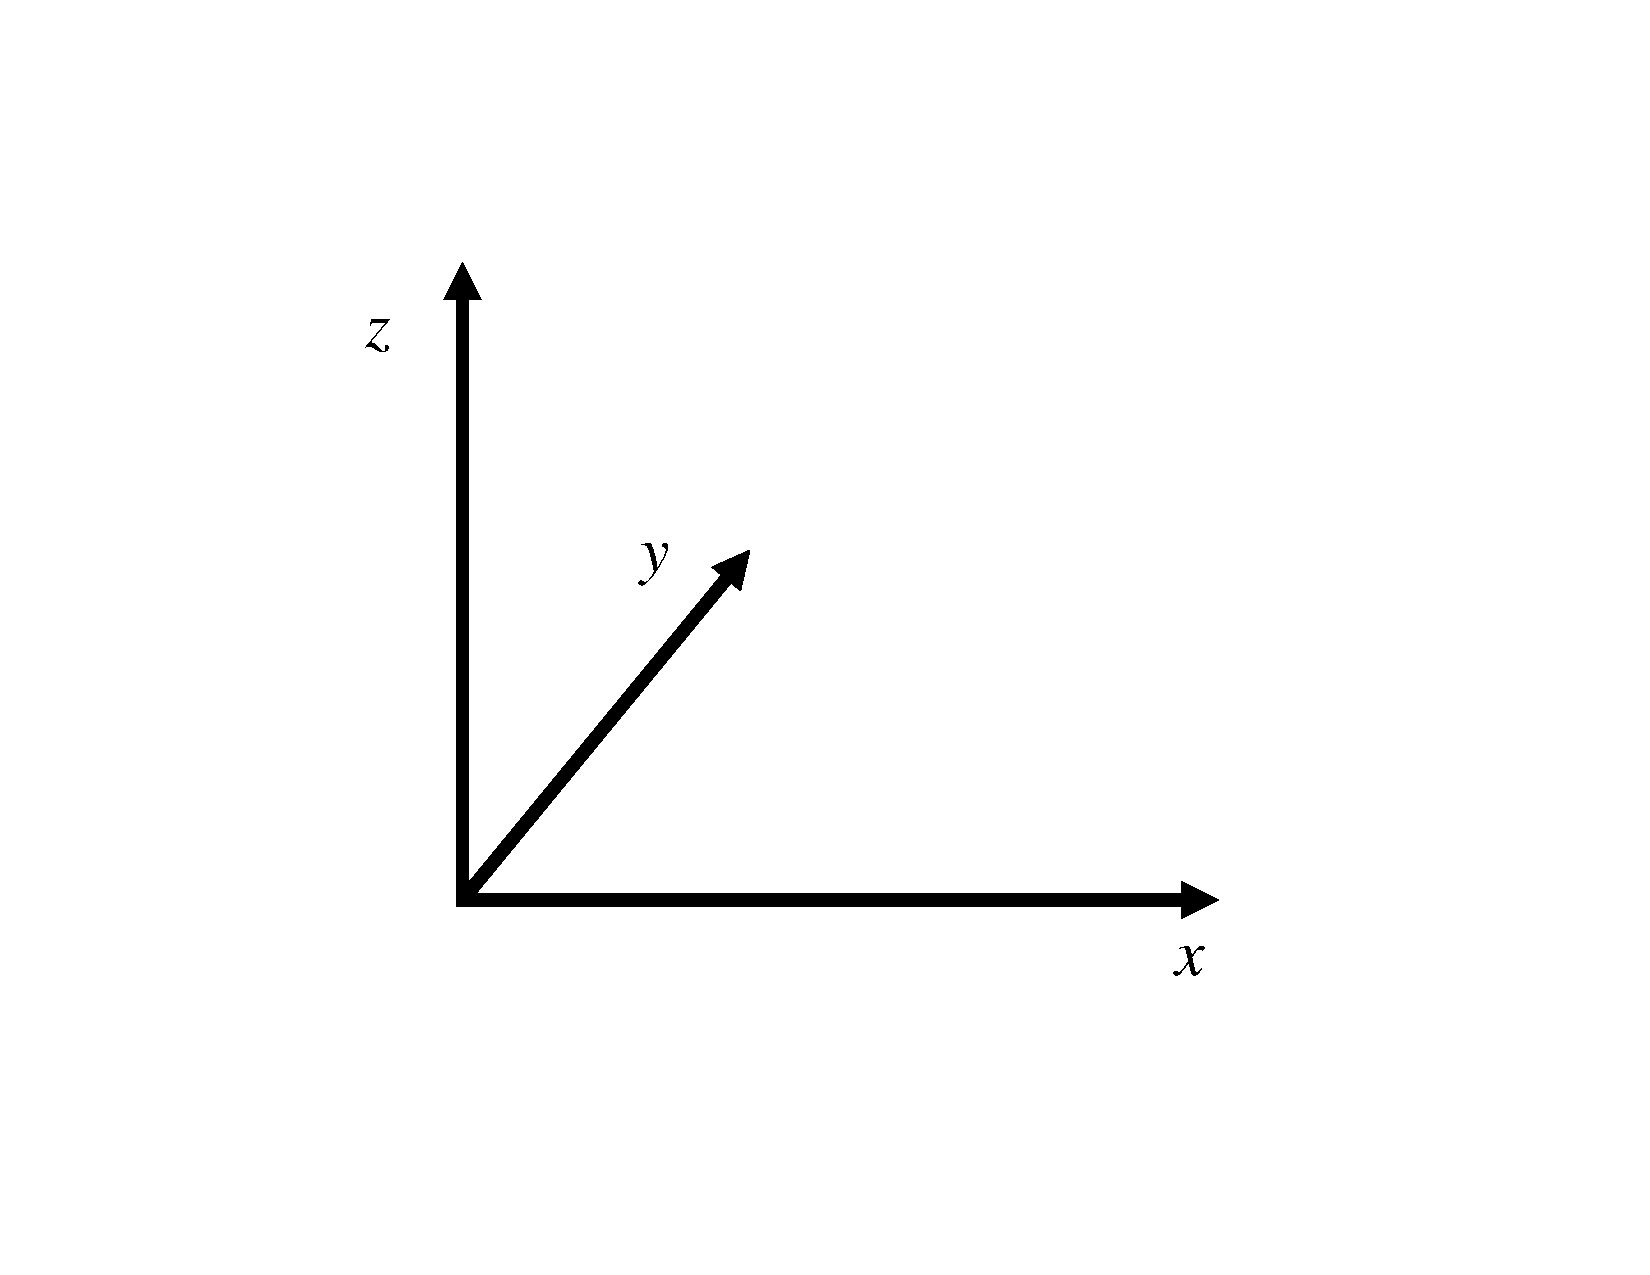
\includegraphics[width=3.0in]{\SMVfigdir/righthandrule}
\end{center}
\caption{Right hand rule used by Smokeview for specifying a 3D vertex locations.}
\label{figrighthand}
\end{figure}

A vertex in OpenGL has the same meaning as in geometry, a
location. Vertices are specified in Smokeview using either {\bf
glVertex3f(x,y,z)}\ or {\bf glVertex3fv(xv)}.  The suffix for
glVertex indicates the number and type of data value to be passed.
For example, {\em 3f}\ is used when passing 3 scalar floating
points.  The suffix {\em 3fv}\ is used to when passing a pointer
(or equivalently a memory address) to 3 floating point  values.

To illustrate, suppose that {\tt xyz}\ is a floating point array
of size 3 containing a 3D coordinate.  One could then use either
of the two OpenGL calls:
\begin{lstlisting}
glVertex3fv(xyz);
glVertex3f(xyz[0],xyz[1],xyz[2]);
\end{lstlisting}
to represent the vertex location.

Groups of vertices may be {\em built up}\ to form more complex
geometric objects. Several objects are illustrated in Fig.
\ref{figshapes}.  They are formed by grouping vertices together
and surrounding them with calls to {\tt glBegin()}\ and {\tt
glEnd()}. The argument passed to {\tt glBegin()}\ determines which
higher level object is drawn. To draw a shaded triangle one would
use
\begin{lstlisting}
glBegin(GL_TRIANGLE);
glVertex3f(0.0,0.0,0.0);
glVertex3f(0.0,1.0,0.0);
glVertex3f(1.0,0.0,0.0);
glEnd();
\end{lstlisting}
Similarly, to draw points or to connect the vertices with lines
(also shown in Fig. \ref{figshapes}) one would replace {\tt
GL\_TRIANGLE}\ above with {\tt GL\_POINTS}\ or {\tt GL\_LINES}\
respectively.
\begin{figure}[bph]
\begin{center}
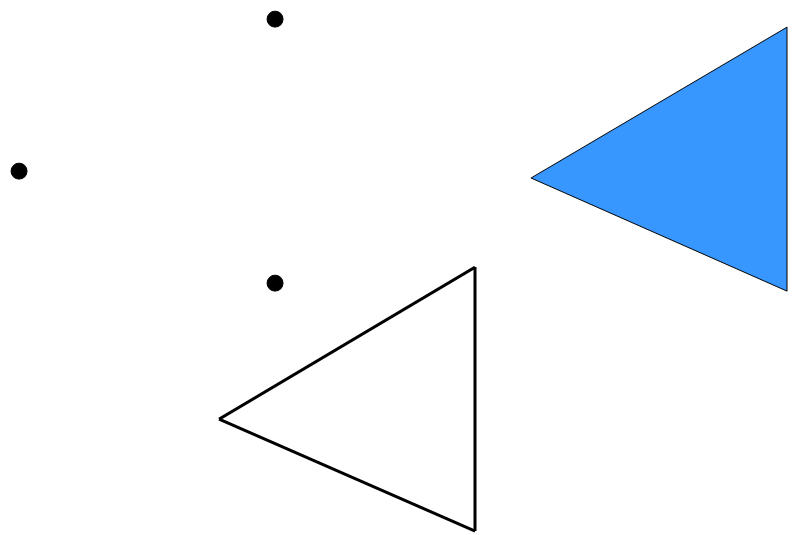
\includegraphics[width=6.0in]{\SMVfigdir/shapes}
\end{center}
\caption[Points, lines and a shaded triangle drawn using OpenGL.]
{Points, lines and a shaded triangle drawn using OpenGL. Vertices
are defined using {\tt glVertex*} and the particular shapes are
generated by passing {\tt GL\_POINTS}, {\tt GL\_LINES}, and {\tt
GL\_TRIANGLE}\ to {\tt glBegin()} } \label{figshapes}
\end{figure}

The triangle is the fundamental construct Smokeview uses to
visualize objects.  To be useful though, these objects need to be
colored, moved and projected onto a 2D terminal screen. These
topics are discussed in the following sections.

%
% -------------------  Setting the Scene ------------------------
%

\subsection{Setting the Scene}
3D objects must be flattened or converted to 2D in order to
display them on a computer screen.  This occurs in two steps.  The
first step is called a projection.  Smokeview uses three kinds of
projections: perspective, orthographic and stereo.  The second
step takes whatever projection that has been applied and maps the
resulting flattened geometry onto a subset of the computer screen.
This window subset, usually a rectangle, is called a viewport. All
viewports in Smokeview are rectangular.

\subsection{Projections}
Projections are used to flatten the 3D scene onto a two
dimensional plane. Two common projections are orthographic and
perspective. An orthographic projection is size preserving.
Objects in the foreground take up the same amount of screen space
as objects in the background. This projection is sometimes called
a parallel projection because parallel lines in the 3D scene
remain parallel when drawn on the screen.

A perspective projection creates an illusion of depth by causing
objects in the background to take up less screen space than the
same sized object drawn in the foreground.  Both projection
methods are available in Smokeview.

Smokeview uses {\tt glFrustum}\ to perform perspective projections
\begin{lstlisting}
      glFrustum(
        (double)fleft,(double)fright,
        (double)fdown,(double)fup,
        (double)fnear,(double)ffar);
\end{lstlisting}
and {\tt glOrtho}\ to perform orthographic projections
\begin{lstlisting}
      glOrtho(
        (double)fleft,(double)fright,
        (double)fdown,(double)fup,
        (double)fnear,(double)ffar);
\end{lstlisting}

\noindent where {\tt fleft}, {\tt fright}, {\tt fdown}, {\tt fup}, {\tt fnear},
{\tt ffar} are six clipping planes bounding the view frustum (truncated pyramid)
for the perspective projection or the box in the orthographic projection.
Drawing does not occur outside of the 3D region defined by these 6 clipping planes.
An additional six clipping planes parallel to the x, y and z axes may be activated
in Smokeview (using the clipping dialog box) to hide geometry making it easier to
see interior objects or visualizations (hence the term clipping plane).  OpenGL
allows one to define clipping planes along arbitrarily oriented planes.
\begin{figure}[bph]
\begin{center}
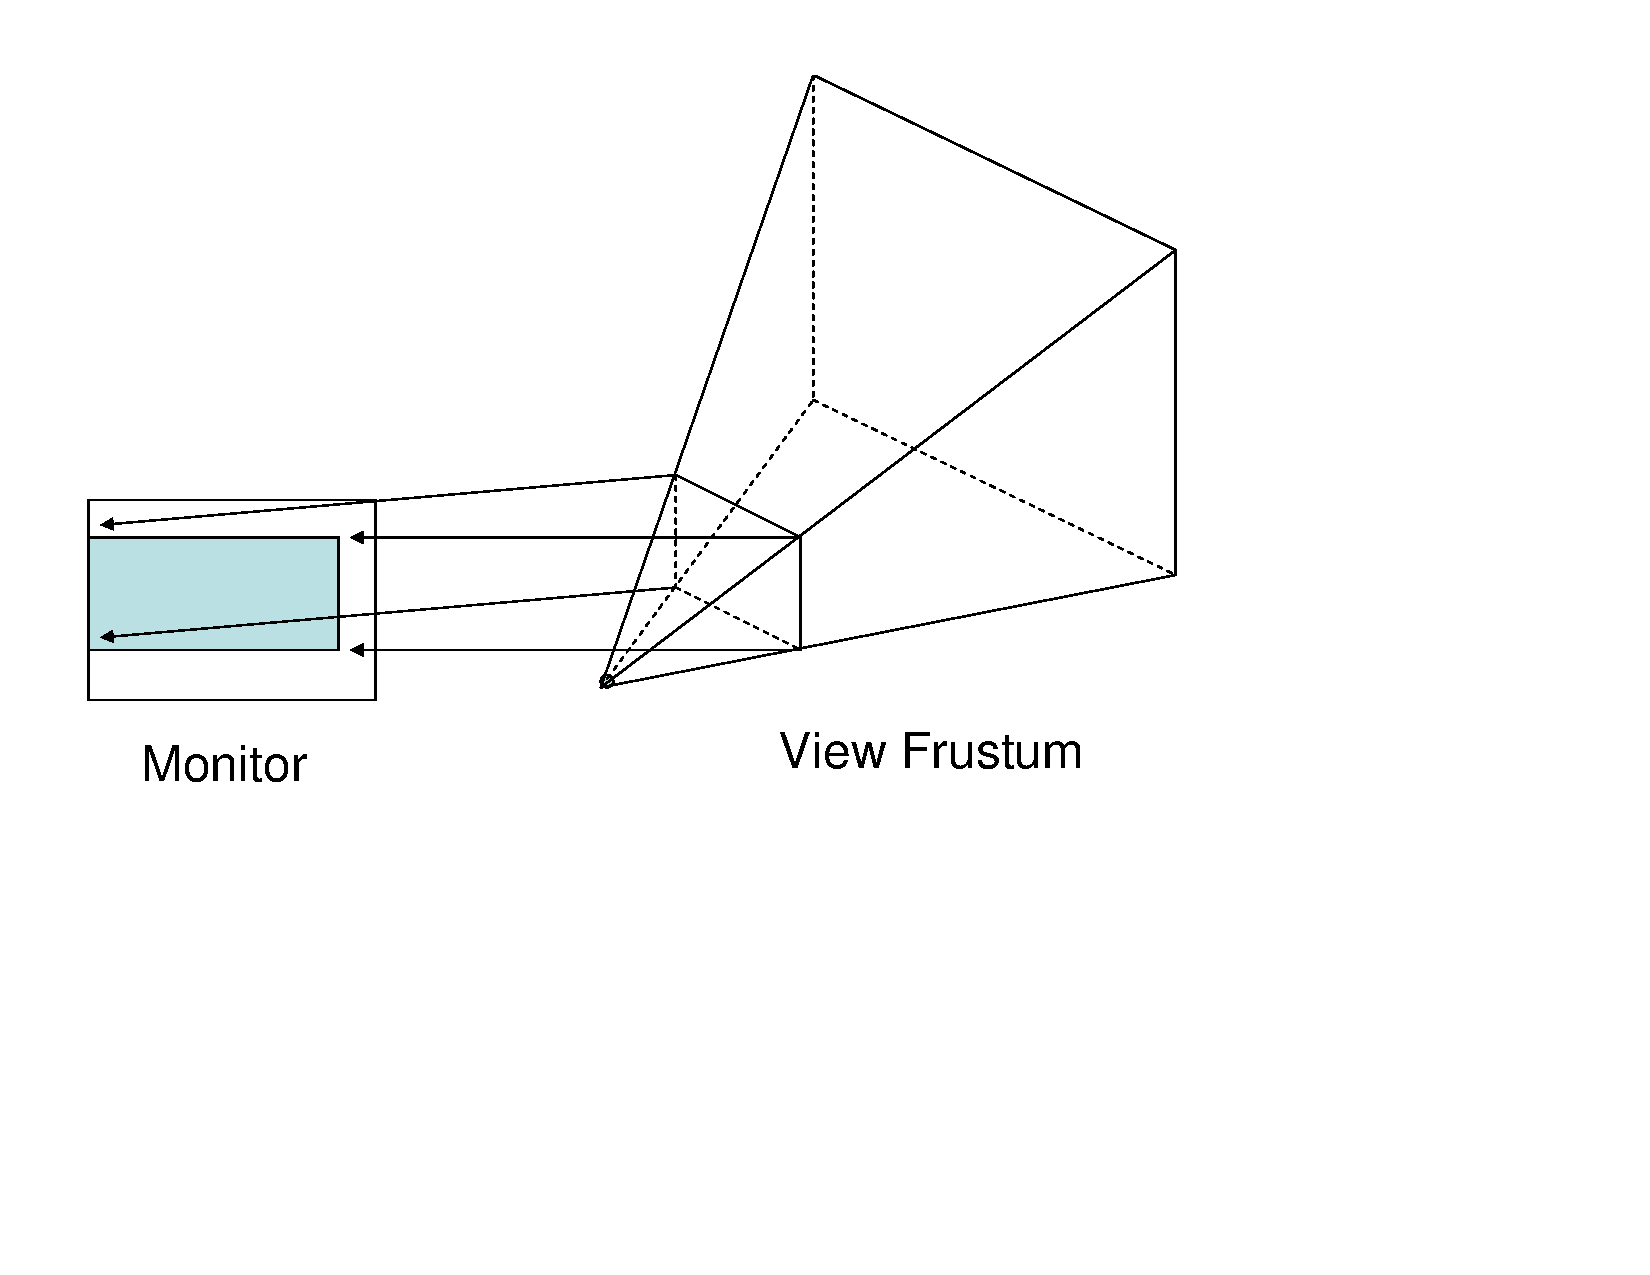
\includegraphics[width=4.0in]{\SMVfigdir/figviewport}
\end{center}
\caption{Example view frustum used to convert 3D scenes to 2D
screen viewport.}
 \label{figfrustum}
\end{figure}

\subsection{Stereo Projections}

A stereo projection is simply a perspective applied twice making adjustments
to simulate the viewpoint as seen for an observer's left and right eye.
The two resulting versions of the scene can then be drawn in succession
using shuttered glasses synced with the monitor to render the stereo effect.
Alternatively, left and right versions of the scene may be drawn at the same
time using stereo viewers to reveal the stereo effect.  Figure \ref{figstereo}
illustrates the two view frustums used for a stereo projection.

\begin{figure}[bph]
\begin{center}
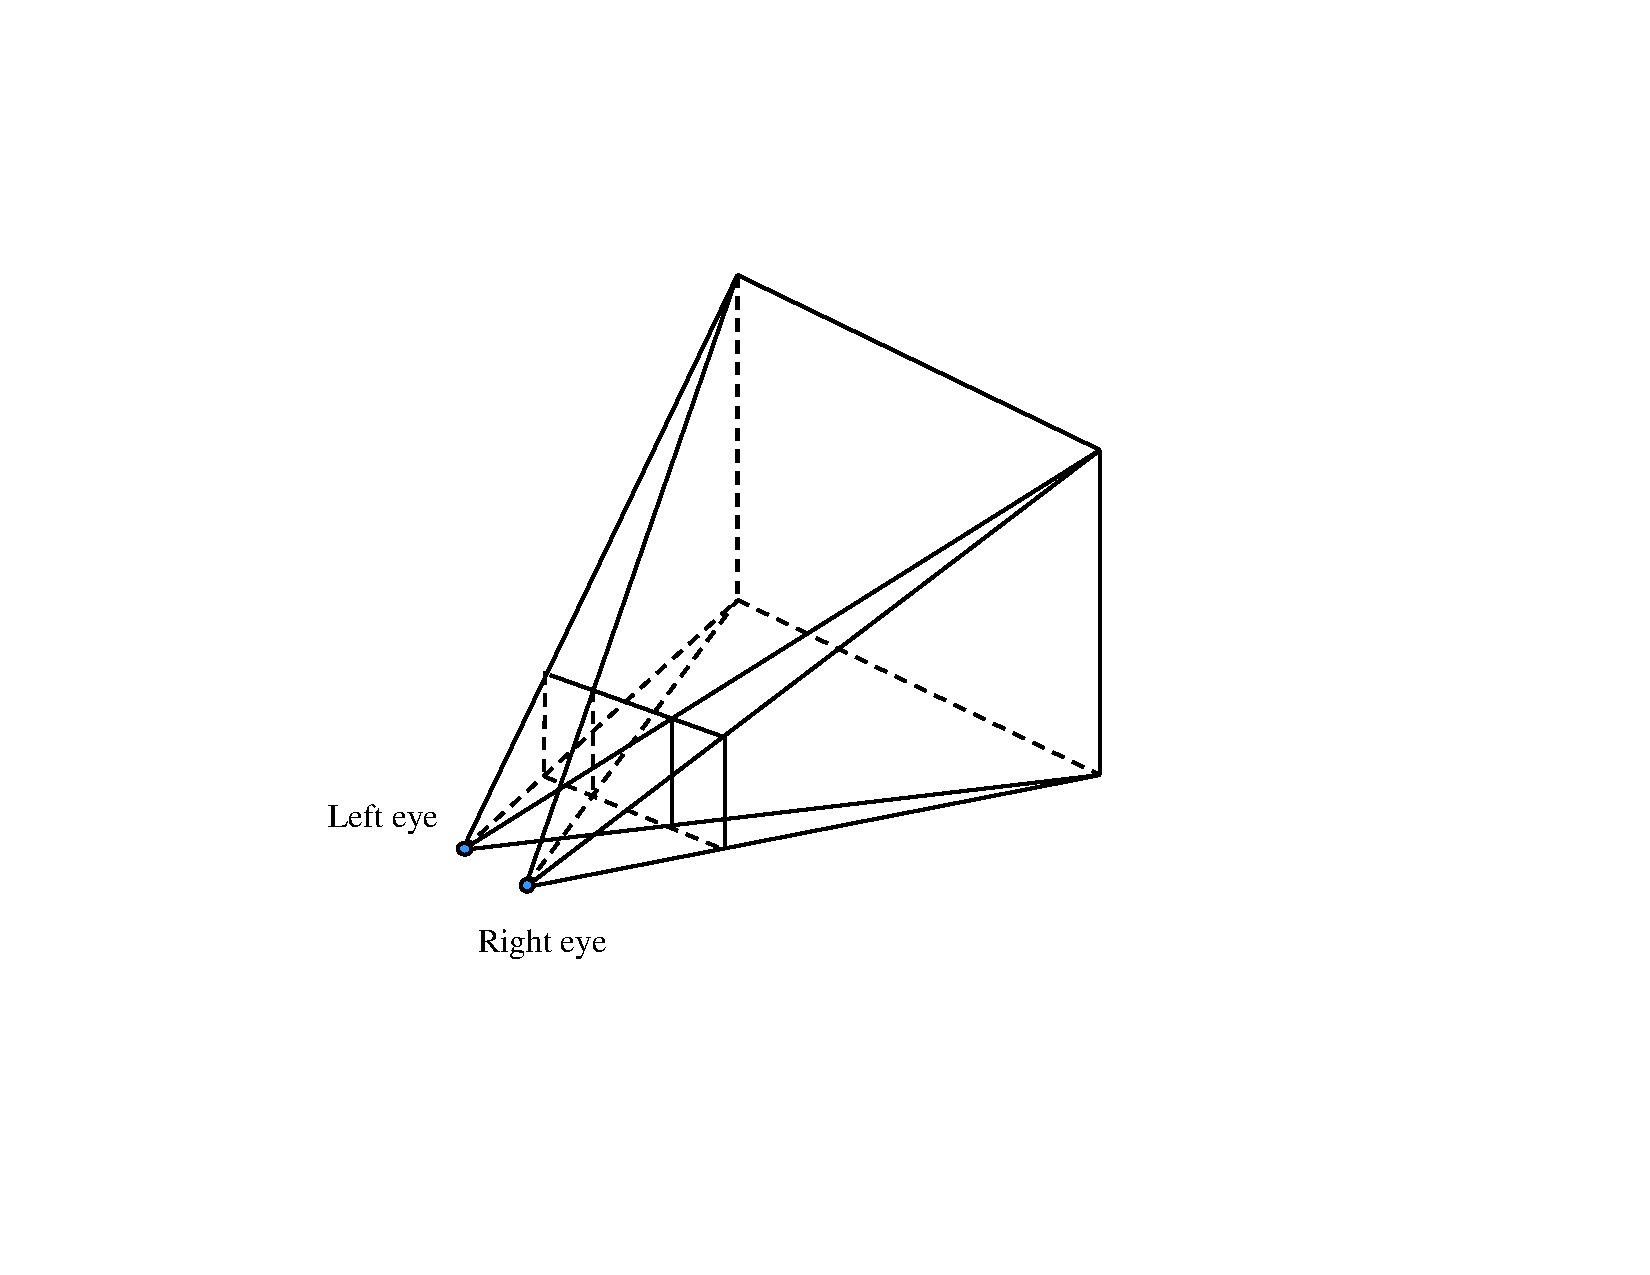
\includegraphics[width=3.0in]{\SMVfigdir/fig_stereo}
\end{center}
\caption{View frustums for stereo pairs.}
 \label{figstereo}
\end{figure}

\subsection{Viewports}
A viewport is the particular portion of the screen where the
drawing occurs.  Smokeview defines separate viewports for drawing
the title, time bar, color bar and the 3D scene.  Figure
\ref{figviewports} illustrates the relationship between the 3D
scene and the 2D screen giving several viewport examples used by
Smokeview.
\begin{figure}[bph]
\begin{center}
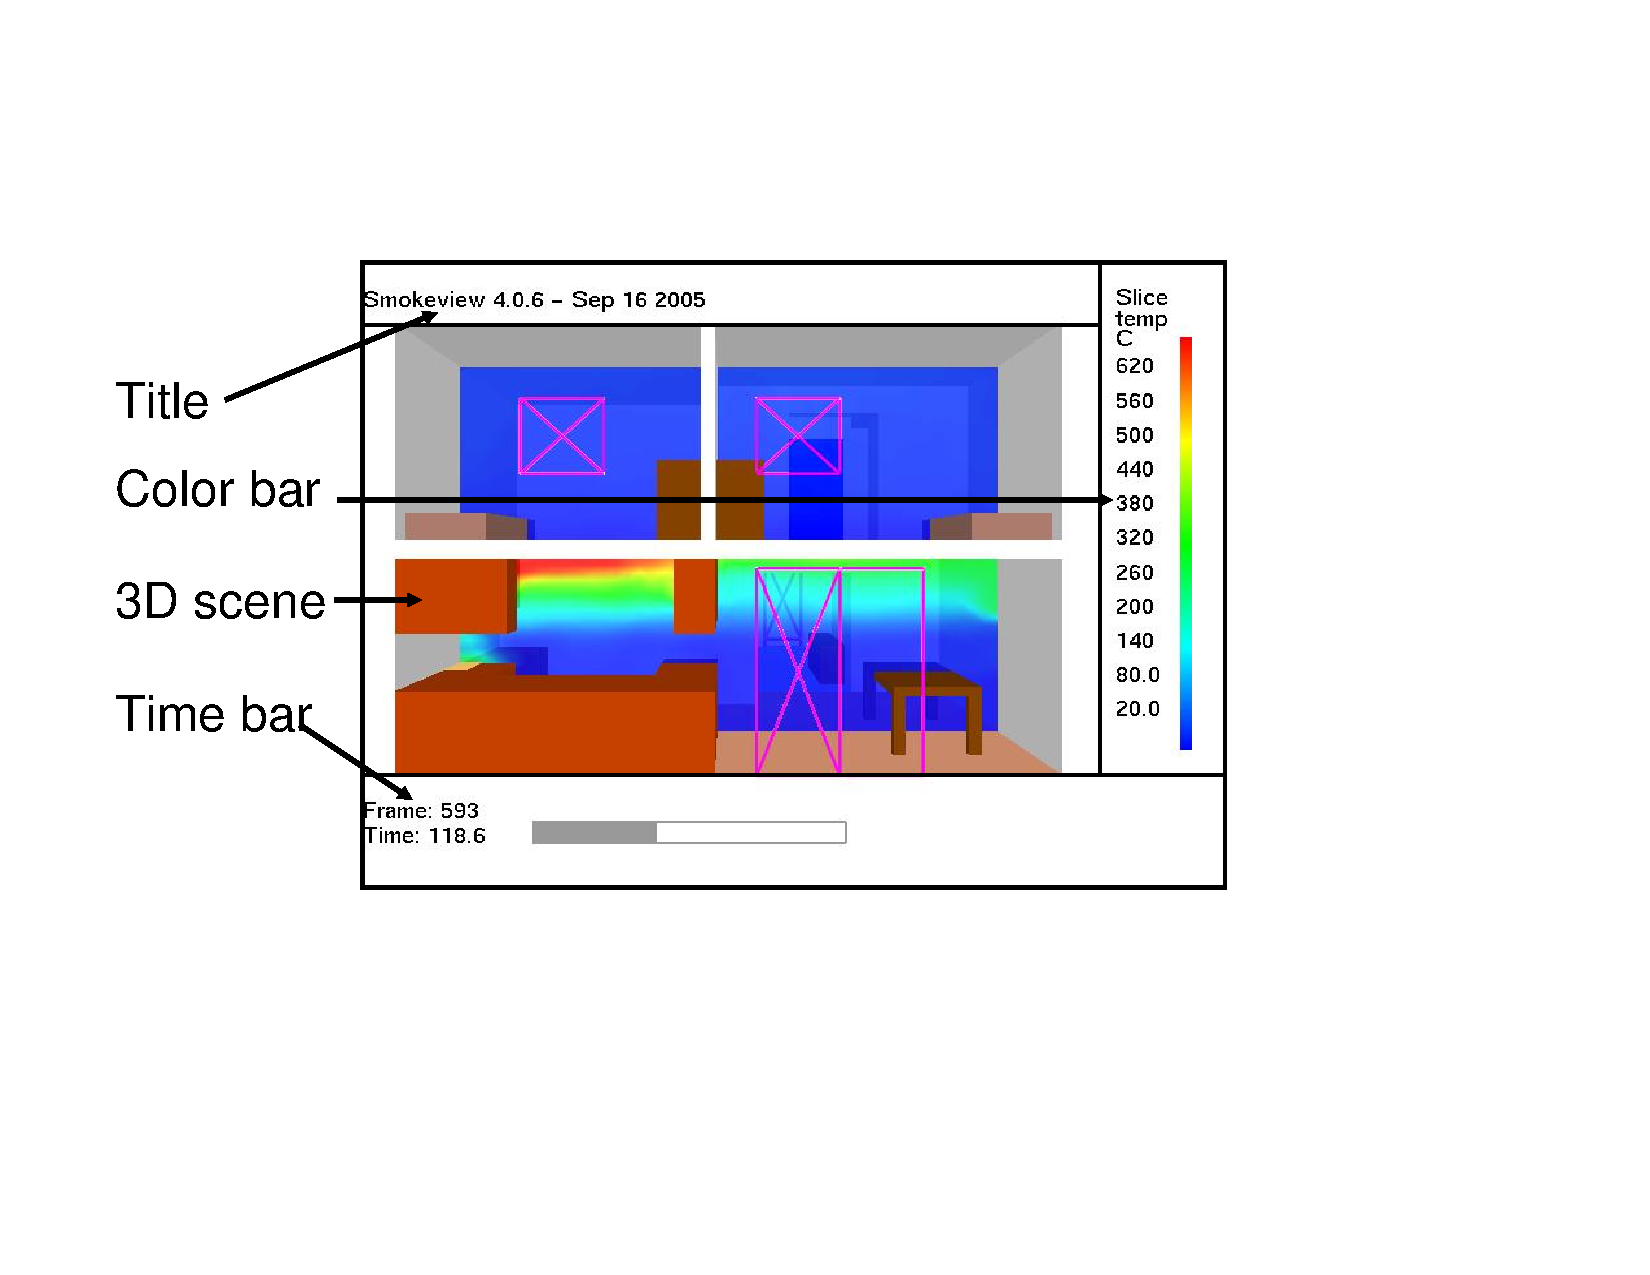
\includegraphics[width=4.0in]{\SMVfigdir/figviewport2}
\end{center}
\caption{Examples of several viewports in a typical Smokeview scene.}
 \label{figviewports}
\end{figure}

Smokeview uses {\tt glViewport()}\ to establish a window viewport.  In particular, the call
\begin{lstlisting}
glViewport(left,down,width,height);
\end{lstlisting}
is used to set up the portion of the screen where 3D drawing occurs where {\tt left}\
and {\tt down}\ are the bottom left screen coordinates of the viewport and {\tt width}\
and {\tt height}\ are the width and height of the viewport.

%
% -------------------  Color, Shading and Blending ------------------------
%

\section{Coloring, Shading and Blending Objects}
Color, shading and blending are three aspects of the same process
used to draw objects residing in a three dimensional environment.
Smokeview uses color to display and more importantly to
distinguish between two or more geometric or data elements.
Shading adds a further depth cue (besides perspective projections
discussed earlier) to present the illusion of 3 dimensions.  Using
a virtual light source, colors are changed subtly based upon the
relative orientation of the light source and the surface being
drawn.  Portions of the surface oriented away from the light are
drawn darker than portions oriented towards the light.  Blending
is the process of combining the colors of two or more objects in
such a way that objects in the background may be seen through
semi-transparent objects drawn in the foreground.  Together,
color, shading and blending add to the illusion that the image
drawn on a two dimensional terminal screen is three dimensional.

\subsection{Color}
Color in OpenGL is defined using four not three components.
Besides the expected components of red, green and blue, OpenGL
uses a component designated as {\em alpha}\ to represent
opaqueness. Each component ranges from 0.0 to 1.0. An alpha
component of 0.0 indicates a color that is completely transparent
while an alpha component of 1.0 represents a color that is
completely opaque.

Colors are specified using the OpenGL routine {\tt glColorXXX()}.
As with {\tt glVertexXXX()}, XXX is replaced by a suffix used to
indicate the number and type of argument passed.  For the most
part, Smokeview uses {\tt glColor3f}, {\tt glColor4f}, {\tt
glColor3fv} and {\tt glColor4fv}.  As before, the 3 or 4 indicates
the number of data values used.  If 3 is specified in the call
then it is tacitly assumed that the fourth component, {\tt alpha},
has value 1.0.  In other words, the color is opaque.  The {\tt f}\
parameter indicates that floating point values are used and the
{\tt v}\ parameter indicates that the variable passed is a pointer
to the actual data to be referenced.

\subsection{Shading} OpenGL uses two shading models for drawing
objects, flat and Gouraud.  These models are specified using {\tt
glShadeModel(GL\_FLAT)}\ and {\tt glShadeModel(gl\_SMOOTH)}\
respectively. Gouraud shading is also referred to as smooth
shading.  Flat shading assumes that objects are drawn in an
environment with uniform lighting - light surrounds an object
equally in all directions. Smooth lighting on the other hand
assumes that light comes from a particular direction.  This causes
subtle changes in color to occur across an object's surface.
Figure \ref{figlighting} shows examples of FDS blockages (the
standard townhouse scenario) drawn using flat and smooth shading.
Flat shading diminishes the three dimensionality of the scene.
\begin{figure}[bph]
\begin{center}
\begin{tabular}{cc}
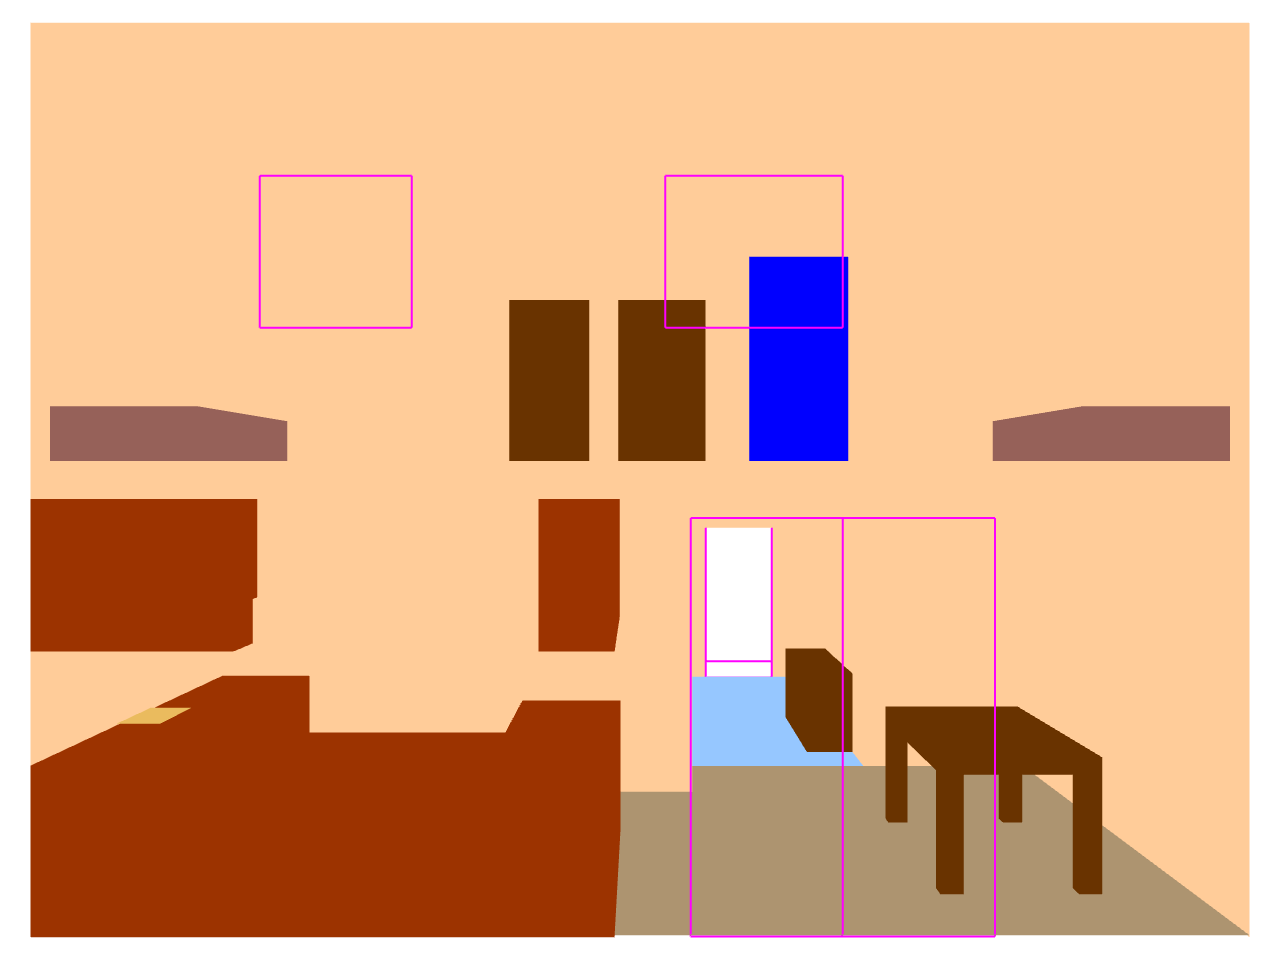
\includegraphics[width=5.0in]{\SMVfigdir/th_unlit}\\
flat shading\\
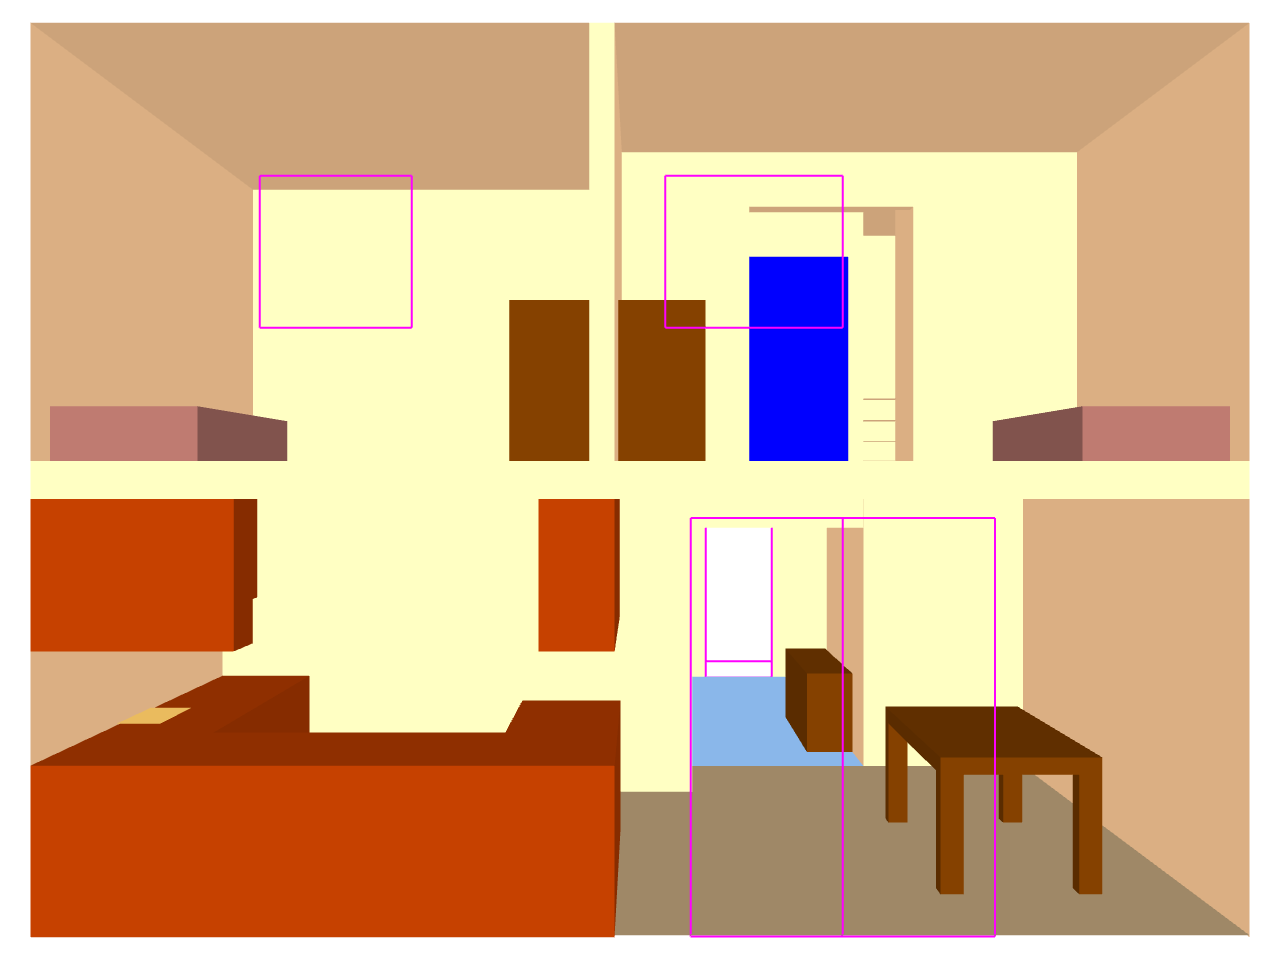
\includegraphics[width=5.0in]{\SMVfigdir/th_lit}\\
smooth (Gouraud) shading\\
\end{tabular}
\end{center}
\caption [The FDS townhouse case drawn using flat and smooth
shading.] { The FDS townhouse case drawn using flat and smooth
shading. All blockage surfaces have identical colors when drawn
with flat shading.  When drawn with smooth shading, blockage
colors change.  Surfaces are darker when not in direct view of the
light source adding to a sense of depth. } \label{figlighting}
\end{figure}

A normal vector, another vertex attribute, is required to
implement a smooth lighting scheme. A normal vector points in a
direction perpendicular to the surface at the vertex. OpenGL uses
this information to estimate the fraction of light from the light
source reflected off of the given surface and intercepted by the
observer.  This is similar to a configuration factor calculation
performed in fire modeling.  The amount of light perceived by the
observer depends on the relative orientation of the light source,
the object (as specified by the location and normal vector of each
vertex) and the observer.

For planar surfaces, the same normal vector is applied to each
vertex defining the surface. For curved surfaces, normal vectors
are determined using an average of the normal directions of faces
surrounding the vertex.  If normals are not averaged then the
discontinuity in slope going from one face or triangle to another
will result in a faceted or gem-like appearance.  Figure
\ref{fignormals} shows examples of drawing using non-averaged and
averaged normals.
\begin{figure}[bph]
\begin{center}
\begin{tabular}{cc}
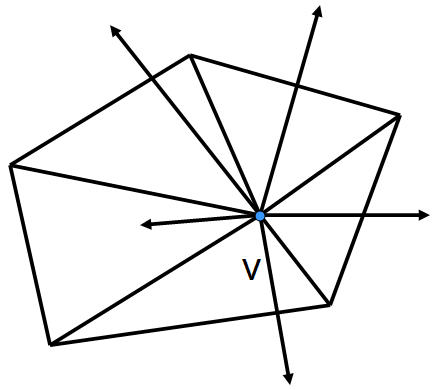
\includegraphics[width=3.0in]{\SMVfigdir/triangle_normal}&
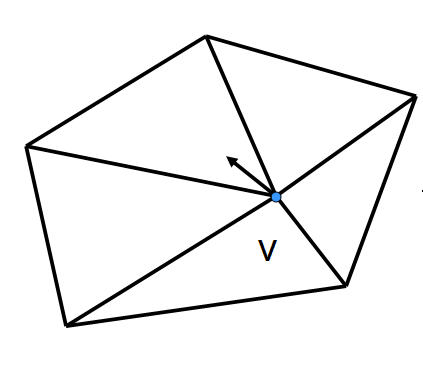
\includegraphics[width=3.0in]{\SMVfigdir/triangle_normal2}\\
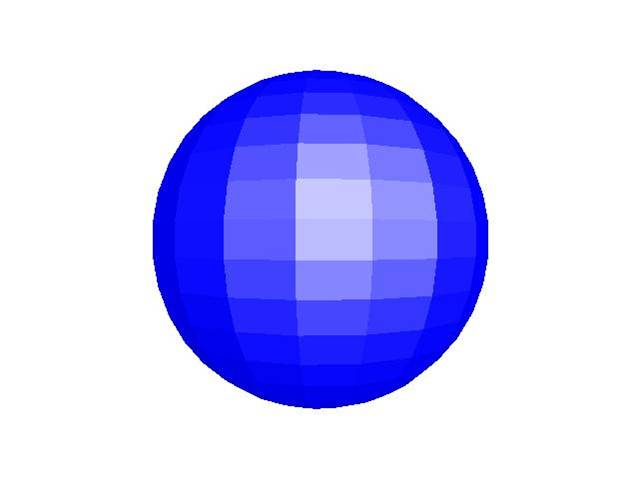
\includegraphics[width=3.0in]{\SMVfigdir/sphere_facet}&
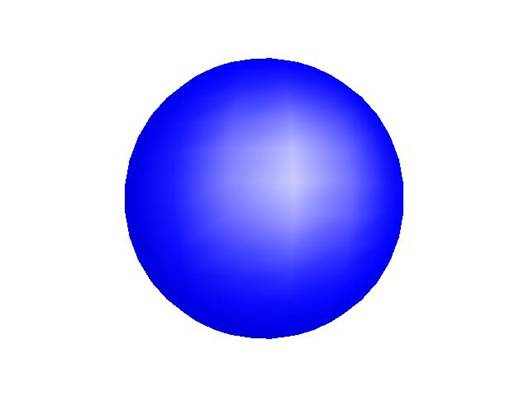
\includegraphics[width=3.0in]{\SMVfigdir/sphere_lit}\\
separate normals $\rightarrow$ faceted drawing&averaged normals $\rightarrow$ smooth drawing\\
\end{tabular}
\end{center}
\caption {Two spheres drawn showing the effect of using averaged
normals.  Using non-averaged normals results in a faceted or
gem-like appearance. } \label{fignormals}
\end{figure}

The Gouraud method for shading then determines a vertex color
using the angle between the light source direction and the vertex
normal vector. The color of the object being shaded is then
determined by interpolating these colors.

Smokeview uses smooth shading or lighting to draw blockages and
iso-surfaces. Particle, slice and boundary files are drawn without
shading as are 3D smoke and Plot3D files.


\subsection{Blending}
\label{blending} Smokeview using OpenGL draws semi-transparent
objects by combining or blending the color of the object currently
being drawn with the color in the current background
buffer.\footnote{The background buffer is updated as each object
is drawn.} The blending fraction is determined from the alpha
color component of the object currently being drawn. A small alpha
results in a small contribution from the currently drawn object
color while a large alpha results in a large contribution.  More
precisely:
\begin{eqnarray}
\noindent\mbox{updated background color} = \alpha\times
\mbox{fragment color} + (1-\alpha)\times \mbox{original background
color}
\end{eqnarray}
This particular blending model is the most common (there are
others) and is activated in Smokeview using the OpenGL call
\begin{lstlisting}
glBlendFunc(GL_ALPHA, GL_ONE_MINUS_SRC_ALPHA);
\end{lstlisting}

Choosing an alpha less than one allows one to {\em see through}\
objects. Smokeview uses this feature to implement partially
transparent blockages and 2D animated slices. Slice files
illustrated in Fig. \ref{figtransparent} are drawn using
transparency. Smokeview also implements data chopping or hiding
using blending or transparency.  Data to be hidden is assigned an
alpha value of 0.0 causing it to be completely transparent.

\begin{figure}[bph]
\begin{center}
\begin{tabular}{c}
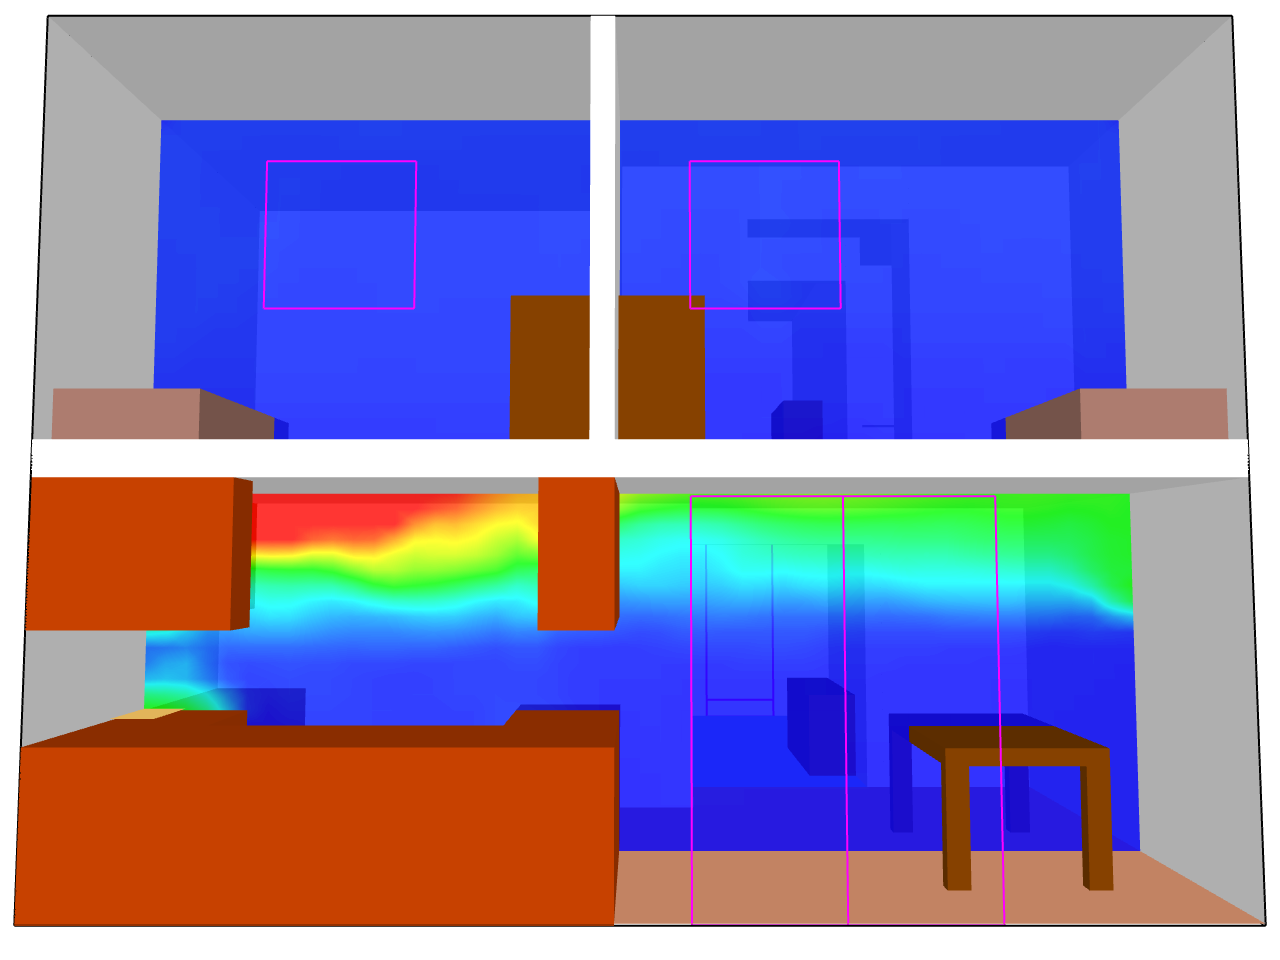
\includegraphics[width=5.0in]{\SMVfigdir/th_transparent}\\
partially transparent slice plane\\
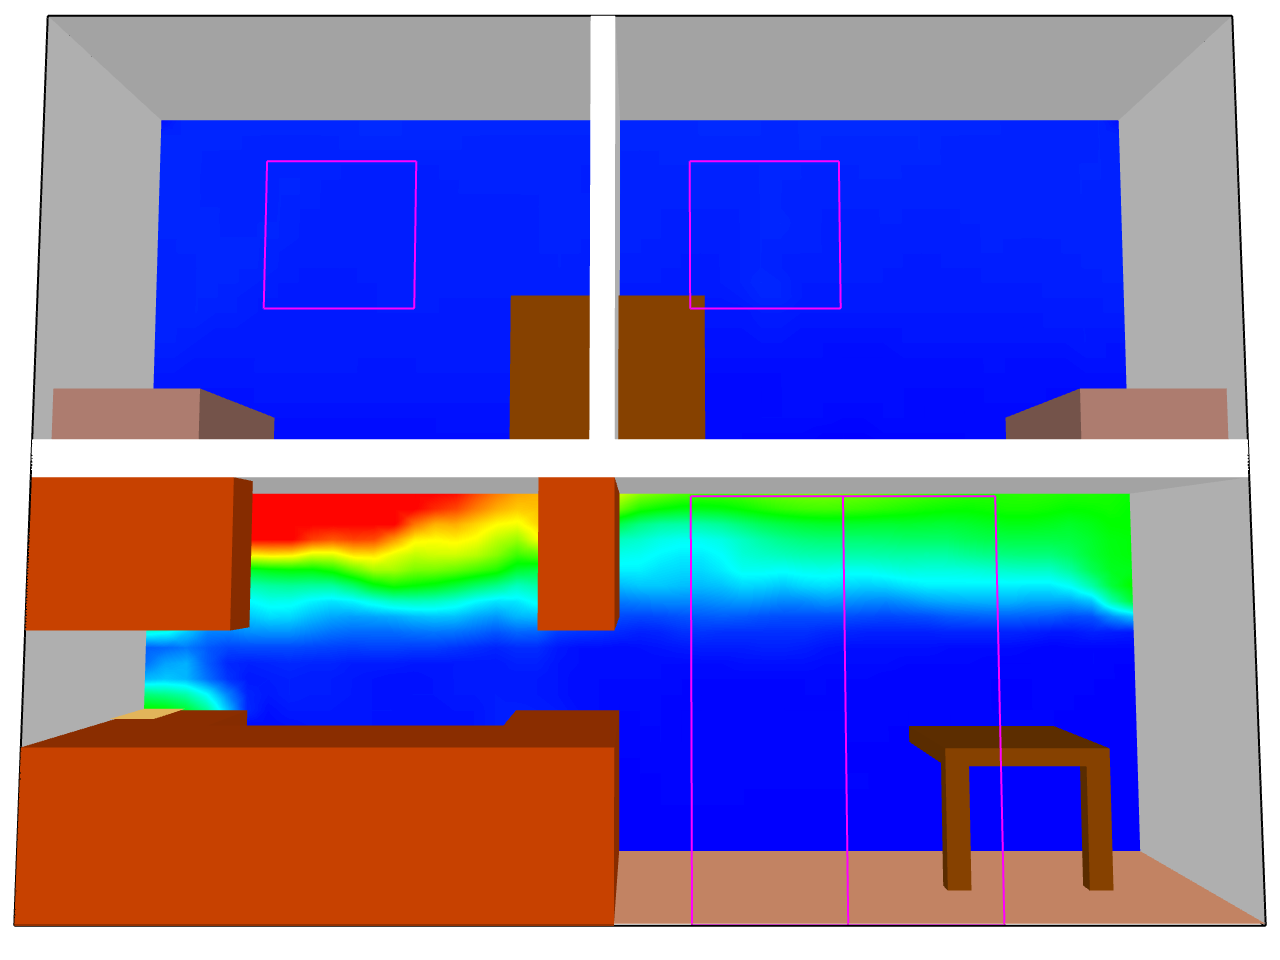
\includegraphics[width=5.0in]{\SMVfigdir/th_solid}\\
opaque slice plane\\
\end{tabular}
\end{center}
\caption {A slice file drawn transparently mixes
slice colors with those in the background.  When drawn opaquely,
any portion of the scene behind the slice file is hidden. }
\label{figtransparent}
\end{figure}

Complications arise, however, because this blending model is not
commutative.  The final color the user sees depends on the order
in which the intermediate colors are drawn. To demonstrate this
simply, consider two objects, one opaque and one semi-transparent.
An opaque object drawn second and in front of a semi-transparent
object will totally obscure the semi-transparent object. A
semi-transparent object drawn second and in front of an opaque
object will blend with but not obscure the opaque object drawn
previously.

To be more precise, consider two objects with colors $c_1$ and
$c_2$ and alpha values $\alpha_1$ and $\alpha_2$.   Let the
background color be denoted $b_0$.  Then blending object 1 with
the background results in a new background color, $b_1$, given by
\begin{eqnarray}
b_1=(1-\alpha_1)b_0 + \alpha_1c_1
\end{eqnarray}
Blending the color $c_2$ with $b_1$ results in a new background color, $b_2$, given by
\begin{eqnarray}
b_2&=&(1-\alpha_2)b_1 + \alpha_2c_2\\
&=&(1-\alpha_2)((1-\alpha_1)b_0 + \alpha_1c_1)+\alpha_2c_2\\
&=&(1-\alpha_2)(1-\alpha_1)b_0 + \alpha_1c_1 + \alpha_2c_2 - \alpha_2\alpha_1c_1
\end{eqnarray}

Now blend colors $c_1$ and $c_2$ to the original background in the
opposite order. Blending the color $c_2$ to with the background
color $b_0$ results in a new background color, $\hat{b}_1$, given
by
\begin{eqnarray}
\hat{b}_1=(1-\alpha_2)b_0 + \alpha_2c_2
\end{eqnarray}
Blending $c_1$ to the interim background color $\hat{b}_1$ results in a new background color,
$\hat{b}_2$, given by
\begin{eqnarray}
\hat{b_2}&=&(1-\alpha_1)\hat{b}_0+\alpha_1c_1\\
\hat{b_2}&=&(1-\alpha_1)((1-\alpha_2)b_0 + \alpha_2c_2)+\alpha_1c_1\\
\hat{b_2}&=&(1-\alpha_1)(1-\alpha_2)b_0 + \alpha_2c_2 + \alpha_1c_1 - \alpha_1\alpha_2c_2
\end{eqnarray}


In general, $b_2-\hat{b}_2=\alpha_1\alpha_2(c_2-c_1)\ne 0$, unless
$c_1=c_2$.  Of course $b_2=\hat{b}_2=0$ if $\alpha_1=0$ or
$\alpha_2=0$ but this is a trivial case in which one of the two
fragments is completely transparent.

The application to Smokeview is that since all smoke is drawn with
the same color, smoke slice plane drawing is order independent.
However, whenever fire is visualized along with smoke, multiple
colors may exist in a given plane (black for smoke, orange for
fire).  In this case, the order that the planes are drawn becomes
important.

In order then to prevent inconsistent drawing for the general
case, opaque objects are drawn first then partially transparent
objects are drawn next from back to front (from the point of view
of the observer). Otherwise transparent objects may appear blended
in front of objects when they should in fact be obscured. Of
significance in Smokeview, is that slice plane ordering is not
important when drawing 3D smoke since all smoke is drawn with the
same color (but different opacities).  However, order is important
when drawing smoke and fire (two different colors) or if
considering more elaborate lighting algorithms where in general
every vertex may have a different color (due to lighting effects).

When lighting is not applied, colors within a triangle are
determined in two steps using bi-linear interpolation. First,
colors along a triangle edge are linearly interpolated using the
two colors of the vertices bounding the edge. Second, the interior
colors are determined along a horizontal scan line again using
linear interpolation using colors previously interpolated on the
triangle edge.

Flat shaded triangles may be drawn more efficiently but are not
effective at visualizing a 3D effect.  More sophisticated shading
techniques are required and are discussed next.

%
% -------------------  Motion ------------------------
%

\section{Motion} Previous sections discussed how appearance is important
in visualization.  This section discusses how motion may be used to gain
insight into fire phenomena.  Motion may be thought of in two separate but
equivalent ways - keeping the scene fixed and changing the observer's location
and view direction or keeping the observer fixed and translating, rotating
and/or scaling the scene.

Objects are moved or translated in OpenGL by applying a transformation to
the current {\bf modelview}\ matrix.  The transformation is a matrix whose
particular form depends on whether it is a translation, a rotation or a scaling.

A translation by $(x,y,z)$ is performed by using {\tt glTranslate3f(x,y,z)}.
This OpenGL call generates the matrix
\begin{eqnarray}
T=\left(%
\begin{array}{cccc}
  1 & 0 & 0 & -x \\
  0 & 1 & 0 & -y \\
  0 & 0 & 1 & -z \\
  0 & 0 & 0 & 1 \\
\end{array}%
\right)
\end{eqnarray}
and applies it to the modelview matrix.

A rotation of $\theta$ degrees about the unit-vector axis, $(x,y,z)$,
is performed using {\tt glRotatef($\theta$,x,y,z)}.  A rotation of
$\theta$ degrees about the $x$~axis is performed using {\tt glRotate($\theta$,1.0,0.0,0.0)}.
This OpenGL call generates the matrix
\begin{eqnarray}
R=\left(%
\begin{array}{cccc}
  1 & 0 & 0 & 0 \\
  0 & \cos(\theta) & -\sin(\theta) & 0 \\
  0 & \sin(\theta) & \cos(\theta) & 0 \\
  0 & 0 & 0 & 1 \\
\end{array}%
\right)
\end{eqnarray}
and applies it to the modelview matrix.

It is of interest to rotate a scene between vectors $u$ and $v$
about an axis perpendicular to both vectors as illustrated in Fig.
\ref{figrotateuv}. The rotation axis is formed by generating the
cross-product of u and v, namely $u\times v$.  The rotation amount
$\theta$ is found using $cos(\theta)=u\cdot v/(||u||\cdot ||v||)$
.  For the special case that $u$ and $v$ are unit vectors and
$u=(0,0,1)$, a vector along the $z$~axis, then $\theta$ and the
rotation axis are given by
\begin{eqnarray}
\theta&=&\cos^{-1}(v_z)\\
u\times v&=&(-v_y,v_x,0)
\end{eqnarray}
so that the OpenGL call to perform the desired rotation would be
{\tt glRotatef}$(180\cos^{-1}(v_z)/\pi,-v_y,v_x,0)$.

\begin{figure}[bph]
\begin{center}
\begin{tabular}{c}
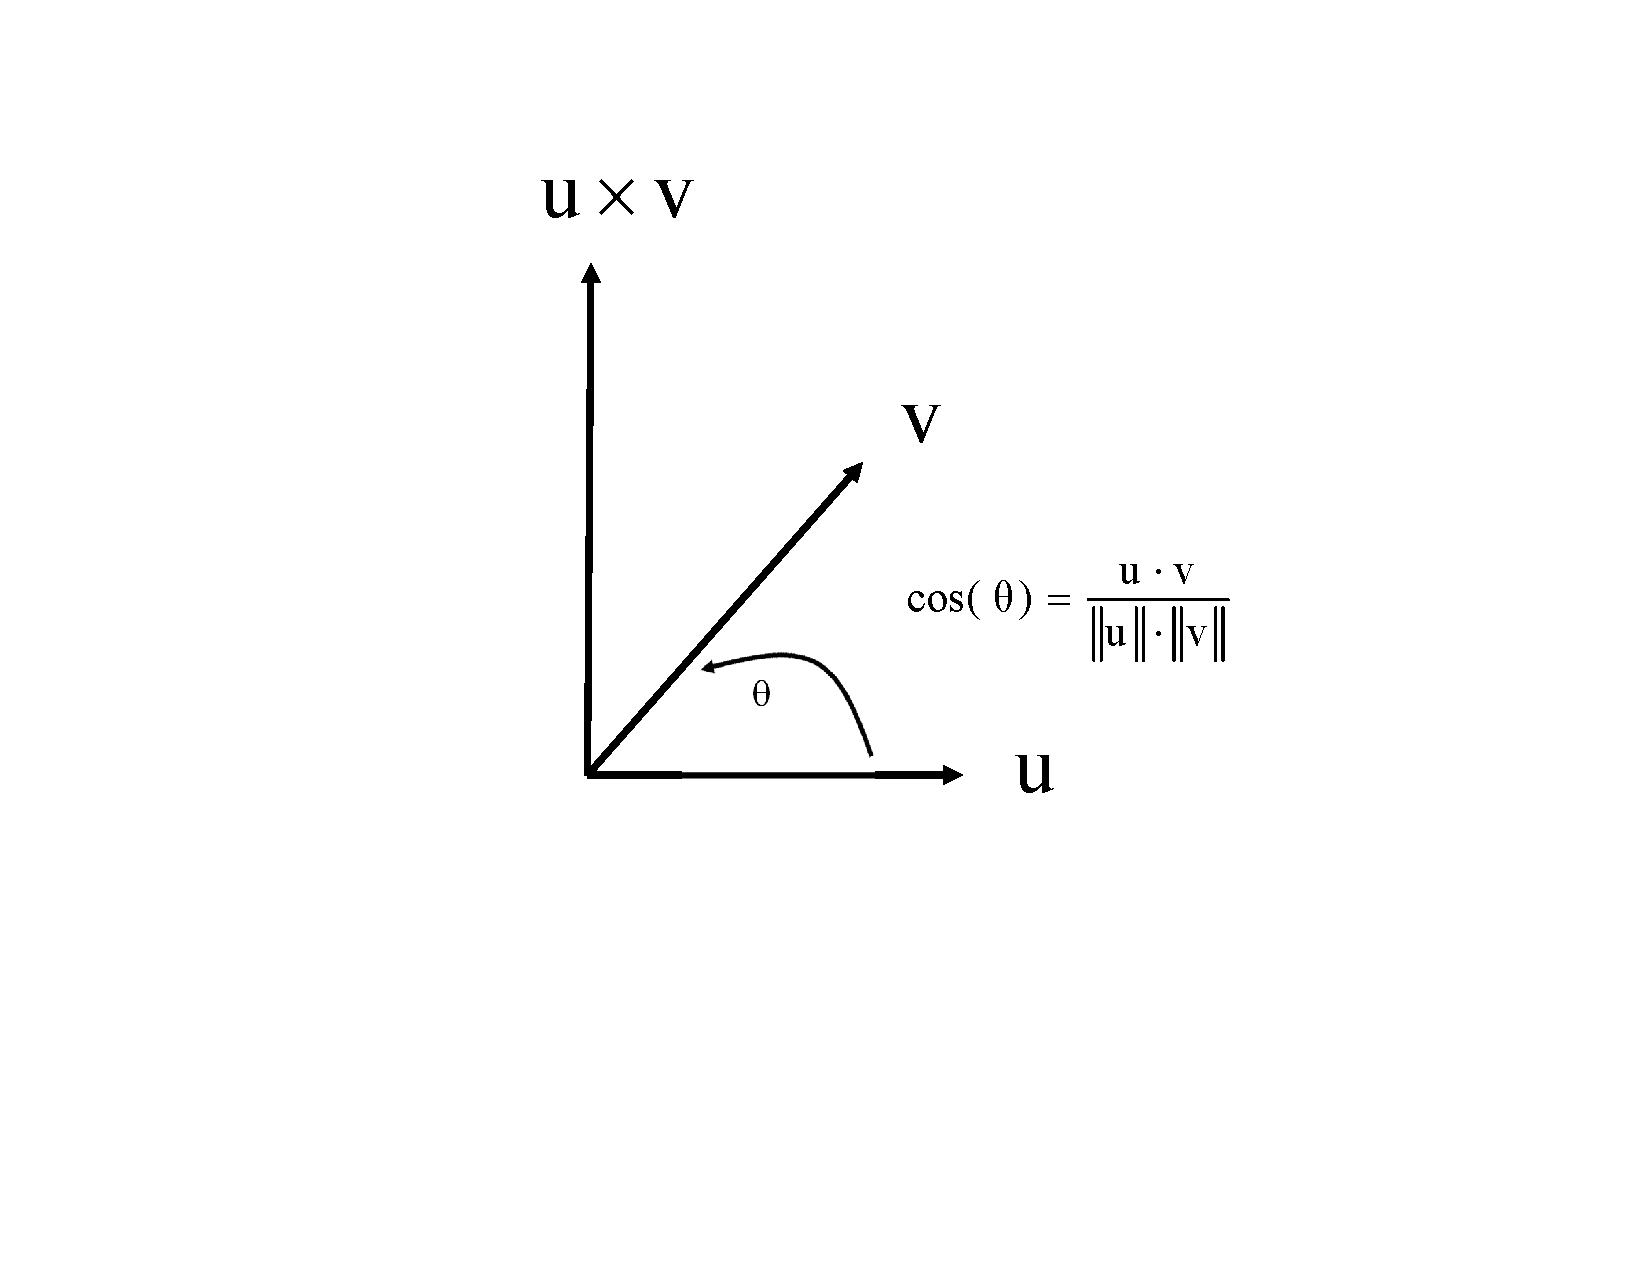
\includegraphics[width=2.5in]{\SMVfigdir/rotate_uv}
\end{tabular}
\end{center}
\caption{Diagram relating the vector $u\times v$ and the angle $\theta$
with vectors $u$, $v$. }
\label{figrotateuv}
\end{figure}

A scaling of $(a,b,c)$ meaning that $x$ components are scaled by
$a$, $y$ components are scaled by $b$, and $z$ components are
scaled by $c$ is performed using {\tt glScale3f(a,b,c)}. This
OpenGL call generates the matrix
\begin{eqnarray}
R=\left(%
\begin{array}{cccc}
  a & 0 & 0 & 0 \\
  0 & b & 0 & 0 \\
  0 & 0 & c & 0 \\
  0 & 0 & 0 & 1 \\
\end{array}%
\right)
\end{eqnarray}
and applies it to the modelview matrix. Smokeview uses scaling to
view cases with large aspect ratios, tunnel fires for example.

This multiplication is usually performed in hardware by the video
card.  The modelview matrix is initialized to the identity matrix
then multiplied by these translation, rotation or scaling
transformation matrices as the scene is moved using the {\tt
glTranslate}, {\tt glRotate}\ and {\tt glScale} OpenGL calls.


\subsection{Implementation}
The desired translation and rotation amounts are communicated
between the user and Smokeview using keyboard and/or mouse
callback routines.  Mouse motion is intercepted by the GLUT mouse
callback routines in Smokeview and named {\tt mouse}\ (first time
mouse is clicked) and {\tt motion}\ (when mouse is pressed and
moving).  GLUT {\em informs}\ the callback of the screen pixel
coordinate which Smokeview uses to determine an elevation or
azimuth angle or a translation amount depending on which control
key (none, CTRL or ALT) is pressed. Smokeview translates and
scales the coordinate system defined in an FDS scenario using
\newcommand{\mmin}{\mbox{min}}
\newcommand{\mmax}{\mbox{max}}
\begin{eqnarray}
\hat{x}&=&(x-x_{\min})/(xyz_{\max}-xyz_{\min})\\
\hat{y}&=&(y-y_{\min})/(xyz_{\max}-xyz_{\min})\\
\hat{z}&=&(z-z_{\min})/(xyz_{\max}-xyz_{\min})
\end{eqnarray}
where $x_{\min}$ and $x_{\max}$ are the smallest and largest $x$
coordinate considering all meshes.  $y_{\min}$, $y_{\max}$,
$z_{\min}$ and $z_{\max}$ are defined similarly.

The Smokeview scene is then translated in this coordinate system
using {\tt glTranslate} using the mouse position as passed to
Smokeview by GLUT.

The Smokeview scene may be rotated about either a vertical or
horizontal axis both passing through the scene center.  The
rotation angle about the horizontal axis (aligned perpendicular to
the viewer's line of sight) is called an elevation angle and the
rotation angle about the vertical axis is called an azimuth angle.
These two angles and the translation amount are used by Smokeview
to control the orientation of the scene.   Rotations are then
implemented in Smokeview using
\begin{lstlisting}
    glTranslatef(xcen,ycen,zcen);
    glRotatef(YZ_AXIS_angle,cos(az_angle),-sin(az_angle),1.0);
    glRotatef(XY_AXIS_angle,0.0,0.0,1.0);
    glTranslatef(-xcen,-ycen,-zcen);
\end{lstlisting}
where {\tt xcen, ycen, zcen}\ are the coordinates of the scene
center, YZ\_AXIS\_angle is the elevation angle, and
XY\_AXIS\_angle is the azimuth angle.  The scene center (center of
rotation) is translated to the origin, requested rotations are
implemented, then the scene is translated back to its original
location.

%
% -------------------  Visualizing Data ------------------------
%

\chapter{Visualizing Data}
Smokeview uses color and contours to visualize data
quantitatively. Color is used to indicate {\em how much}\ of a
quantity is at a given location whereas contours are used to
identify {\em where}\ rather than {\em how much}\ a specified
quantity occurs.

Coloring methods for visualizing data work by assigning colors
based upon data values to various vertices within the scene. These
vertices coincide with the FDS grid, either within a horizontal or
vertical plane (slice or Plot3D file) or on a blockage exterior
(boundary file).  The video card then interpolates these colors at
the interior of the figure, usually a triangle, formed by the
vertices. Coloring variations result from differing methods for
interpolating color between the vertices, either interpolating
within the 3D color cube or using a 1D texture map (the colorbar).

Smokeview uses {\em marching}\ algorithms for generating contours,
marching squares for generating 2D contours and marching
cubes~\cite{marchingcubes} for generating 3D contours. {\em
Marching}\ algorithms work by reducing the general contouring
problem to that of finding the contour in an elementary figure
such as a square or a cube.  Marching squares are used for finding
2D contours in a plane and marching cubes are used for finding
isosurfaces in a volume. A contour for a region is then generated
by splitting the region into a series of squares for 2D contours
or a series of cubes for a 3D contour and finally assembling the
contour acquired from all the parts.

Smokeview uses two methods for representing Smokeview flow data
realistically.  The first involves particles, representing smoke
flow by tracking tracer particles as they move through the
simulation influenced by an underlying  velocity field.  This
velocity field and the particle motion is computed by FDS and
communicated to Smokeview using data files.  This was the first
method Smokeview implemented for visualizing smoke flow and was
inspired by the software tool named Frames written by James Sims.

The second method for visualizing smoke flow involves a method
known as volumetric rendering.  Smoke transparency is visualized
using the optical properties of soot noting that the amount
of light obscured by smoke and hence its shade depends on
the quantity of smoke between the observer and the background.
Smokeview then integrates the smoke opacity one grid plane at a
time using a simple implementation of Beer's law in the video
hardware.



%
% -------------------  Coloring Data ------------------------
%

\section{Coloring Data}
Smokeview uses several methods to visualize data quantitatively
involving converting data values to color. The basic procedure is
to
\begin{enumerate}
\item obtain minimum and maximum data bounds to use in scaling,
either through calculation or specification by the user,

\item map data onto integer indices between 0 to 255 ,

\item obtain colors using indices computed in step 2 to index into
a color table (a numerical representation of the color bar)

\item display colors using 1D texture maps (or {\tt glColorxx}\ in
the case of particles).
\end{enumerate}
These steps are detailed in the following sections.   It is
important to point out that the use of 1D texture maps in step 4
enables more detail to be obtained from the visualization due to
the way that color interpolations between grid points are
performed.

\subsection{Determining Data Bounds}Smokeview uses three methods for
setting data bounds.  First, the bounds may be set by the user.
This would be useful to ensure consistent coloring when several
file types are displayed simultaneously (say slice and boundary files).
A second method is to use {\em percentile}\ bounds (1st and 99th by default)
which are useful when data outliers are present.  To find percentile bounds,
Smokeview scans the data computing a histogram.  It then picks data bounds at
a specified percentile levels, 1st and 99th by default.  The third method for
setting data bounds is to simply pick the global bounds for the data.

\subsection{Converting data to a color}
An index into a color table of size 256 is computed using

\begin{eqnarray}
\mbox{color index}=\left\{
\begin{array}{ll}
  0 & v < v_{min}\\
  1+253(v-v_{min})/(v_{max}-v_{min}) & v_{min}\le v \le v_{max} \\
  255 & v > v_{max}
\end{array}
\right.
\end{eqnarray}

\noindent where $v_{min}$ and $v_{max}$ are specified data bounds.
Each table entry contains 4 components (red, green, blue and
opacity).  Each component is scaled from 0.0 to 1.0.  The data in
the colorbar data structure then defines colors (by default) as
illustrated by the {\bf bold path}\ in Fig. \ref{colorbarinfo}.
Other colorbars may be used, for example a color bar containing
shades of gray from white to black.


\begin{figure}[bph]
\begin{center}
\begin{tabular}{cc}
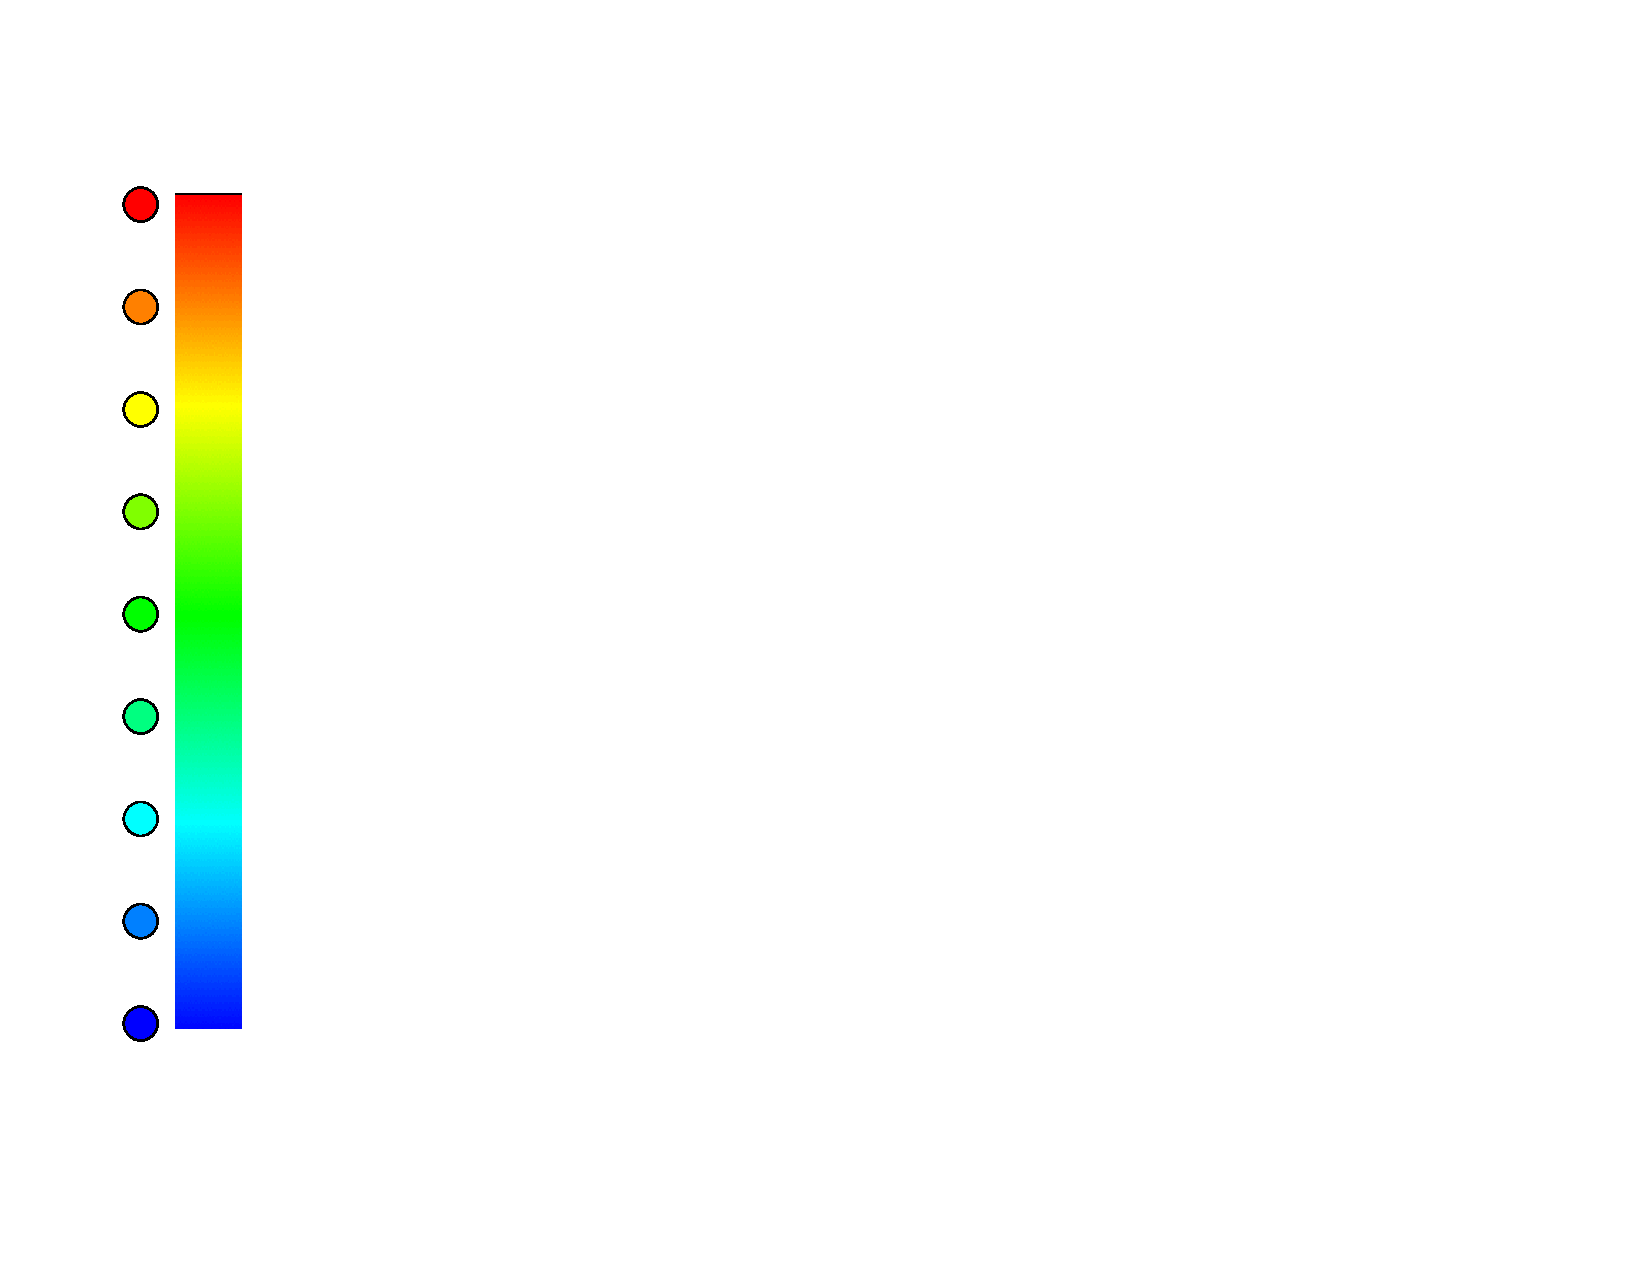
\includegraphics[height=4.0in]
{\SMVfigdir/rainbowcolor}&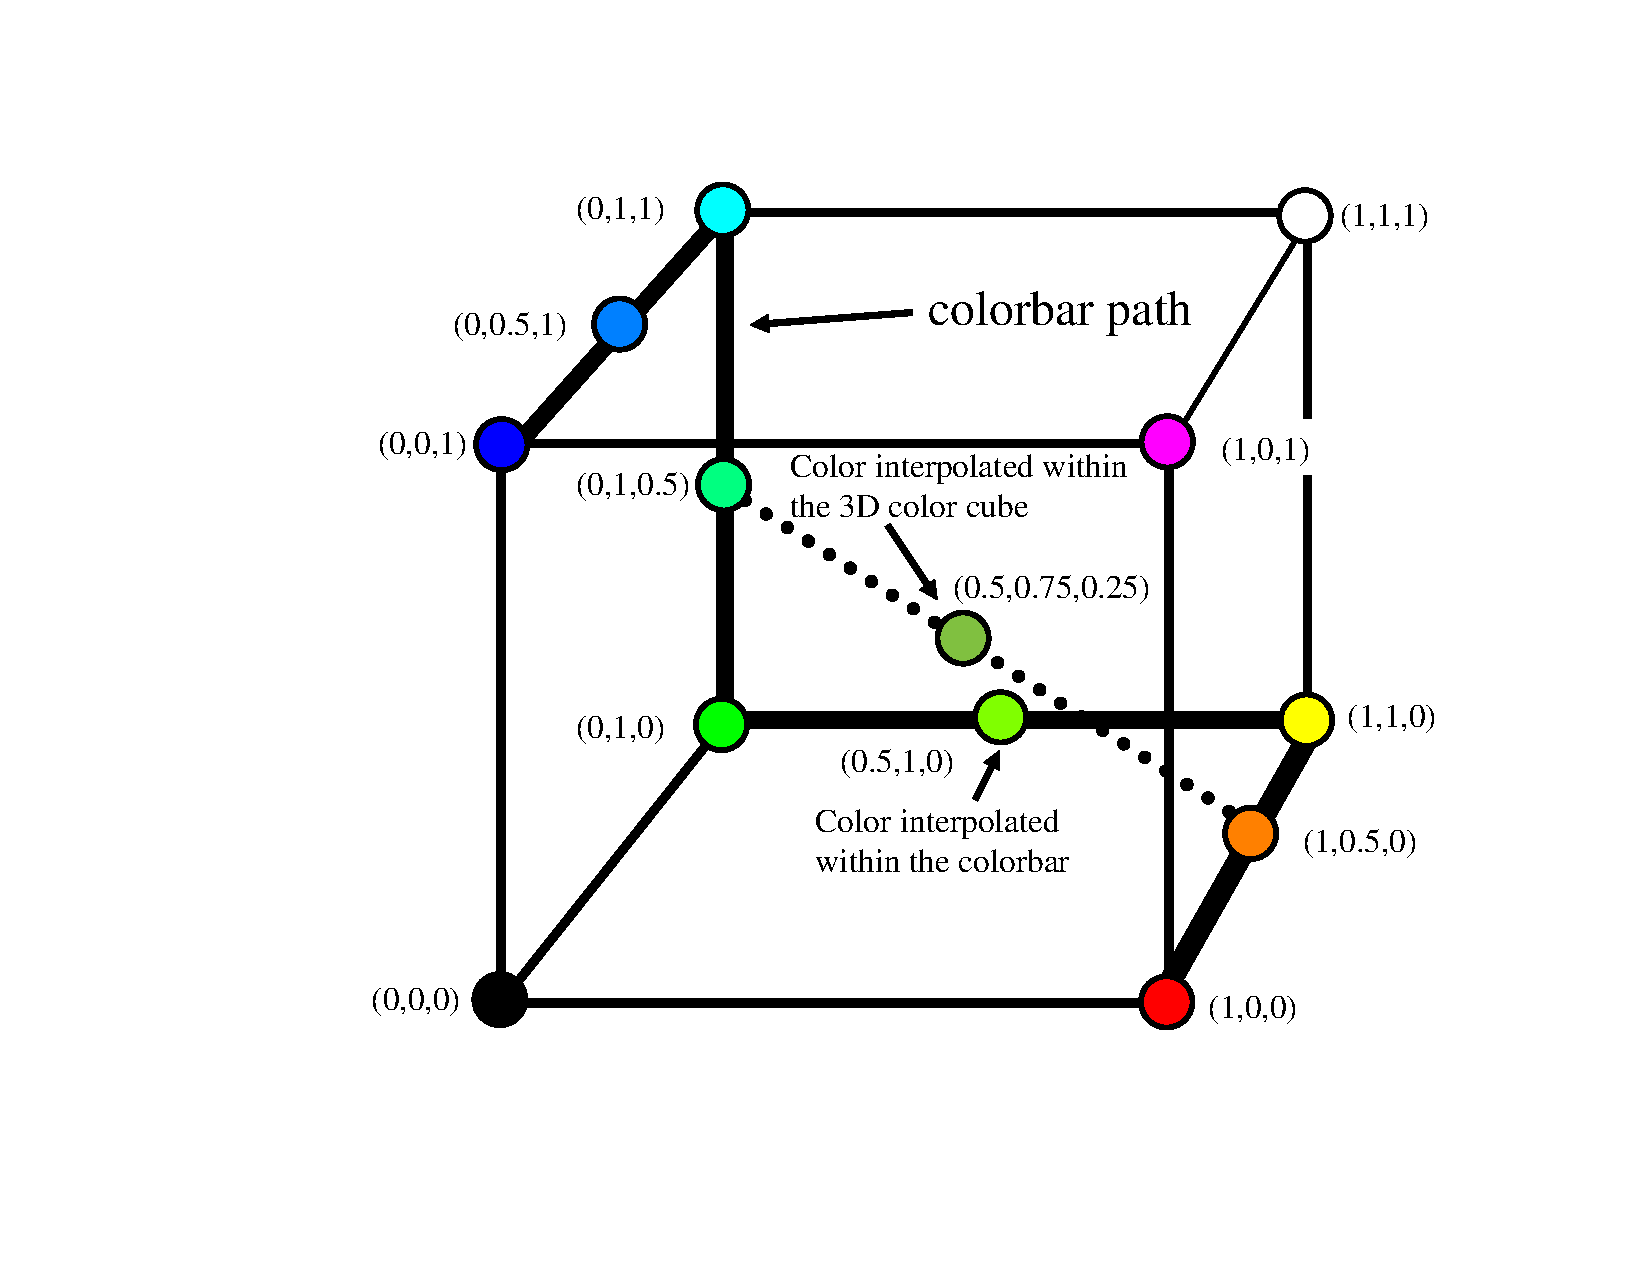
\includegraphics[height=4.0in]{\SMVfigdir/3dcolorcube}\\
a) colorbar&b) 3D color cube\\
\end{tabular}
\end{center}
\caption[1D colorbar and 3D color cube]{The 1D colorbar on the
left is mapped onto the 3D color cube along the {\bf bold path}
from blue to cyan to green to yellow to red.  Colors interpolated
within the cube are different than colors interpolated within the
colorbar.}
\label{colorbarinfo}%
\end{figure}

\subsection{Interpolating Colors}

Consider the following code segment for drawing a shaded triangle
with red, green and blue vertices:
\begin{lstlisting}
glBegin(GL_TRIANGLE);
glColor3f(1.0,0.0,0.0);
glVertex3f(0.0,0.0,0.0);

glColor3f(0.0,1.0,0.0);
glVertex3f(0.0,1.0,0.0);

glColor3f(0.0,0.0,1.0);
glVertex3f(1.0,0.0,0.0);
glEnd();
\end{lstlisting}

OpenGL interpolates colors between the vertices and interior to
the triangle using the color cube as in Fig. \ref{colorbarinfo}.
For example, if two vertices A and B are colored $(0.0,1.0,0.5)$
and $(1.0,0.5,0.0)$, then a point half way in between would be
colored $(0.5,0.75,0.25)$, the average of the two colors.  This
color is the midpoint of the line segment AB interior to the color
cube.

Smokeview version 4 (and earlier) uses this method, interpolating
data within the 3D color cube (not the colorbar).  As a result,
near the fire or wherever there are large temperature gradients,
interpolation artifacts occur.  For example, if a red (1,0,0)
region occurs near a blue (0,0,1) region, the interpolated color
halfway in between would be (0.5,0.0,0.5), a shade of purple, not
in the colorbar.  In general, suppose that $ci_j$ is an integer
index between 0 and 255 and that $f(ci_j)$ is the $ci_j$'th color
in the colorbar.  Then the interpolated color between the
two colors $f(c_1)$ and $f(c_2)$ would be
\begin{eqnarray}
\mbox{interpolated color}=(f(c_1)+f(c_2))/2
\end{eqnarray}

This is not a good method for displaying colors related to data
since only data on the colorbar have physical meaning.  By using
1D texture maps, color indices are interpolated not colors.
Therefore, colors displayed in data plots are always contained in
the colorbar which is what we want.

Smokeview interpolates color indices not colors. As a result,
interpolated colors are contained in the colorbar.  This
interpolation method is implemented using 1D texture maps.  A 1D
texture map is defined using the desired colorbar.  A texture
coordinate is assigned to each data vertex.    Color indices at
pixels between vertices are interpolated using the texture
coordinate.  In general, Smokeview uses the scheme,
\begin{eqnarray}
\mbox{interpolated color}=f((c_1+c_2)/2)
\end{eqnarray}
where $c_1$ and $c_2$ are color indices as before.

The following code segment sets up the use of 1D texture map.

\begin{lstlisting}
  glTexEnvf(GL_TEXTURE_ENV,GL_TEXTURE_ENV_MODE,GL_REPLACE);
  glEnable(GL_TEXTURE_1D);
  glBindTexture(GL_TEXTURE_1D,texture_slice_colorbar_id);
\end{lstlisting}

The following code segments (simplified) shows an example of drawing a slice in a YZ plane.

\begin{lstlisting}
   for(j=jmin; j<jmax; j++){
     for(k=kmin; k<kmax; k++){
       glTexCoord1f( r11); glVertex3f(xplane, yy1,  z1);
       glTexCoord1f( r31); glVertex3f(xplane,  y3,  z1);
       glTexCoord1f(rmid); glVertex3f(xplane,ymid,zmid);

       glTexCoord1f( r31); glVertex3f(xplane,  y3,  z1);
       glTexCoord1f( r33); glVertex3f(xplane,  y3,  z3);
       glTexCoord1f(rmid); glVertex3f(xplane,ymid,zmid);

       glTexCoord1f( r33); glVertex3f(xplane,  y3,  z3);
       glTexCoord1f( r13); glVertex3f(xplane, yy1,  z3);
       glTexCoord1f(rmid); glVertex3f(xplane,ymid,zmid);

       glTexCoord1f( r13); glVertex3f(xplane, yy1,  z3);
       glTexCoord1f( r11); glVertex3f(xplane, yy1,  z1);
       glTexCoord1f(rmid); glVertex3f(xplane,ymid,zmid);
     }
   }
   glEnd();
\end{lstlisting}



Figure \ref{fignewslice} shows the old and new method for
coloring.  Note that the new method results in crisper, clearer
colors. Fig. \ref{colorinterp} illustrates two methods for
interpolating color.  Colors are interpolated in Fig.
\ref{colorinterp}a within the color cube where the colors within
the cube have value (r,g,b).  Colors are interpolated in Fig.
\ref{colorinterp}b with the colorbar.

\begin{figure}[bph]
\begin{center}
\begin{tabular}{cc}
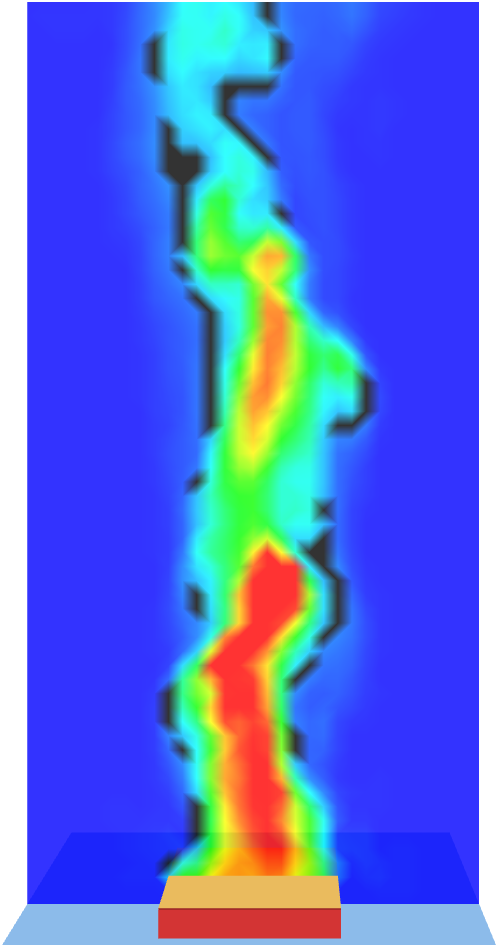
\includegraphics[width=3.0in]
{\SMVfigdir/plume_bad}&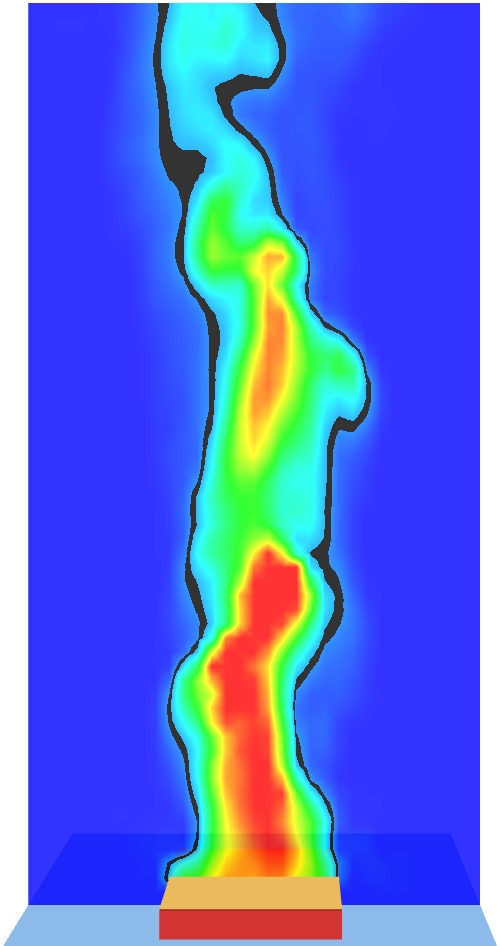
\includegraphics[width=3.0in]{\SMVfigdir/plume_good}\\
interpolate colors within a 3D color cube&interpolate colors within 1D texture color bar\\
\end{tabular}
\caption [Slice file snapshots illustrating old and new method for
coloring data.] {Slice file snapshots illustrating old and new
method for coloring data.}
\label{fignewslice}%
\end{center}
\end{figure}



\begin{figure}[bph]
\begin{center}
\begin{tabular}{c}
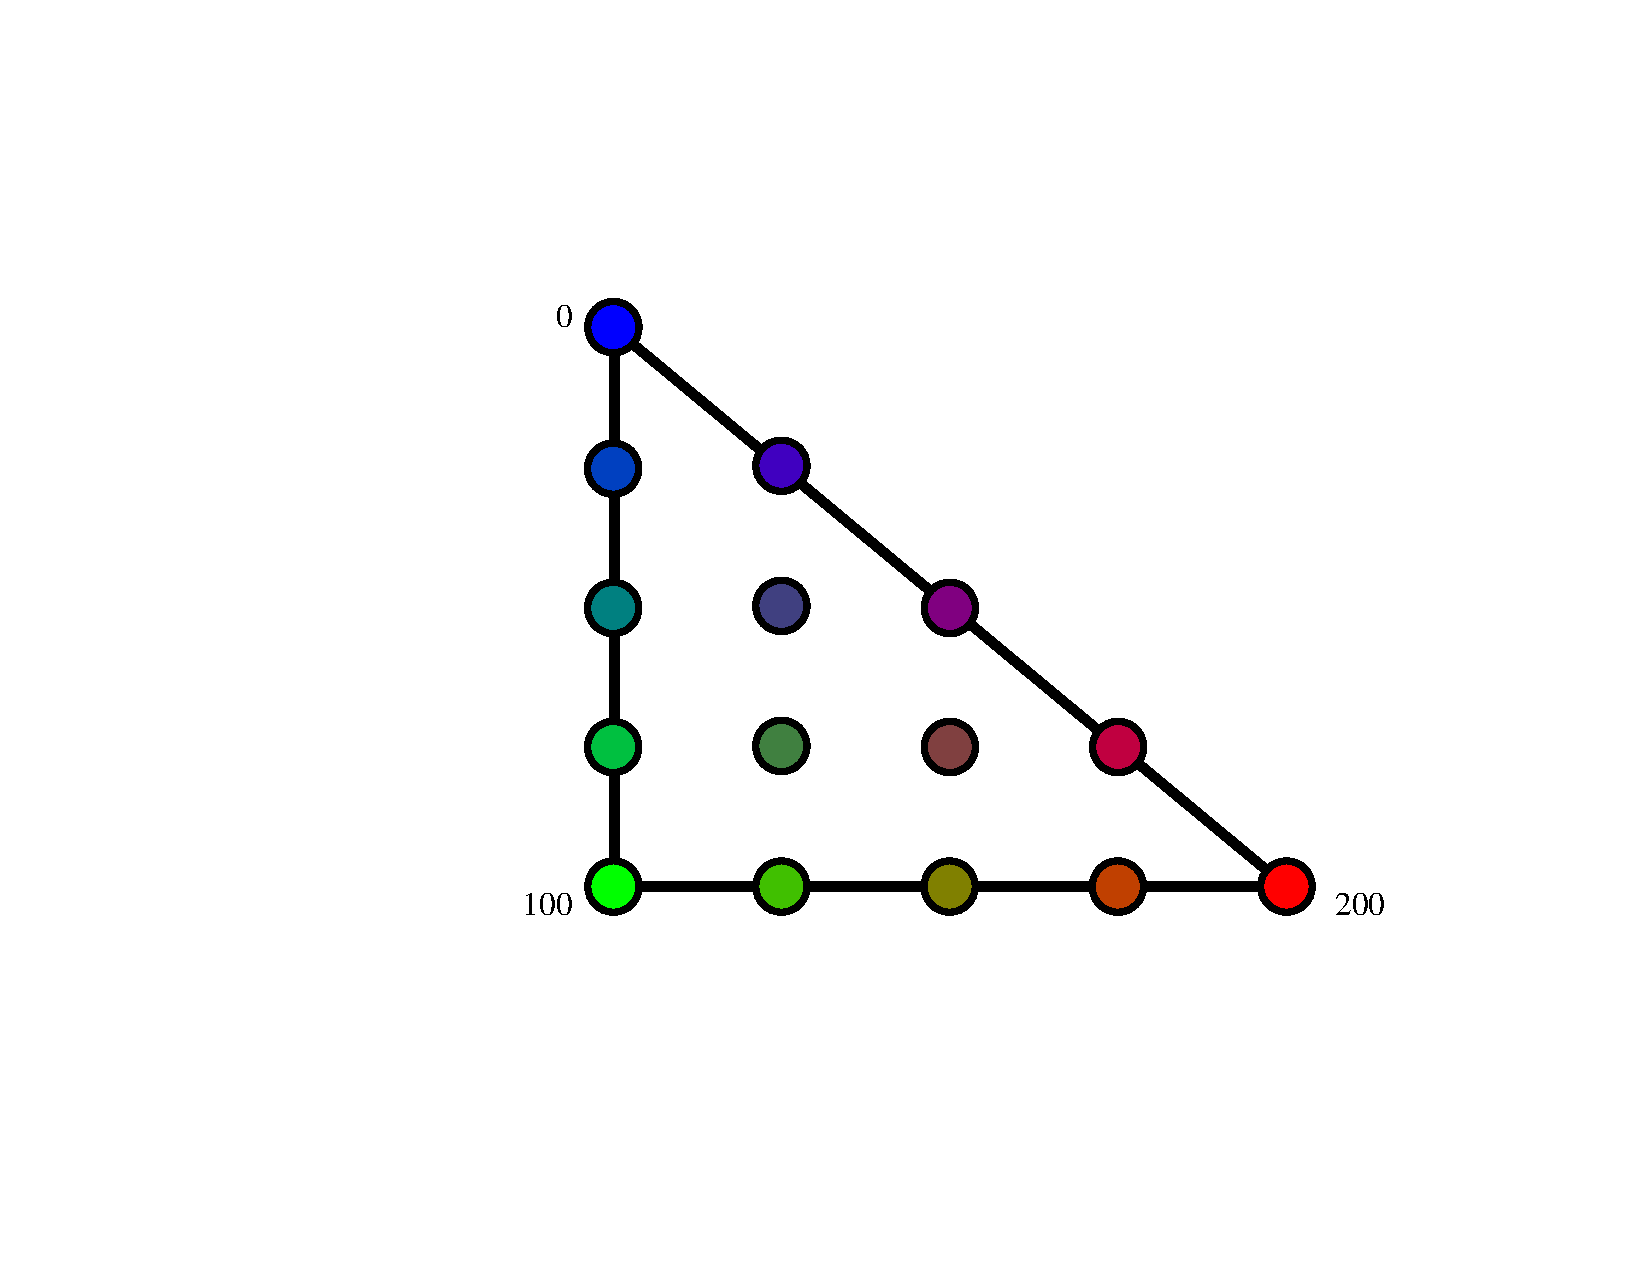
\includegraphics[height=4.0in]{\SMVfigdir/interpcolorrgb}\\
a) colors interpolated within the color cube\\
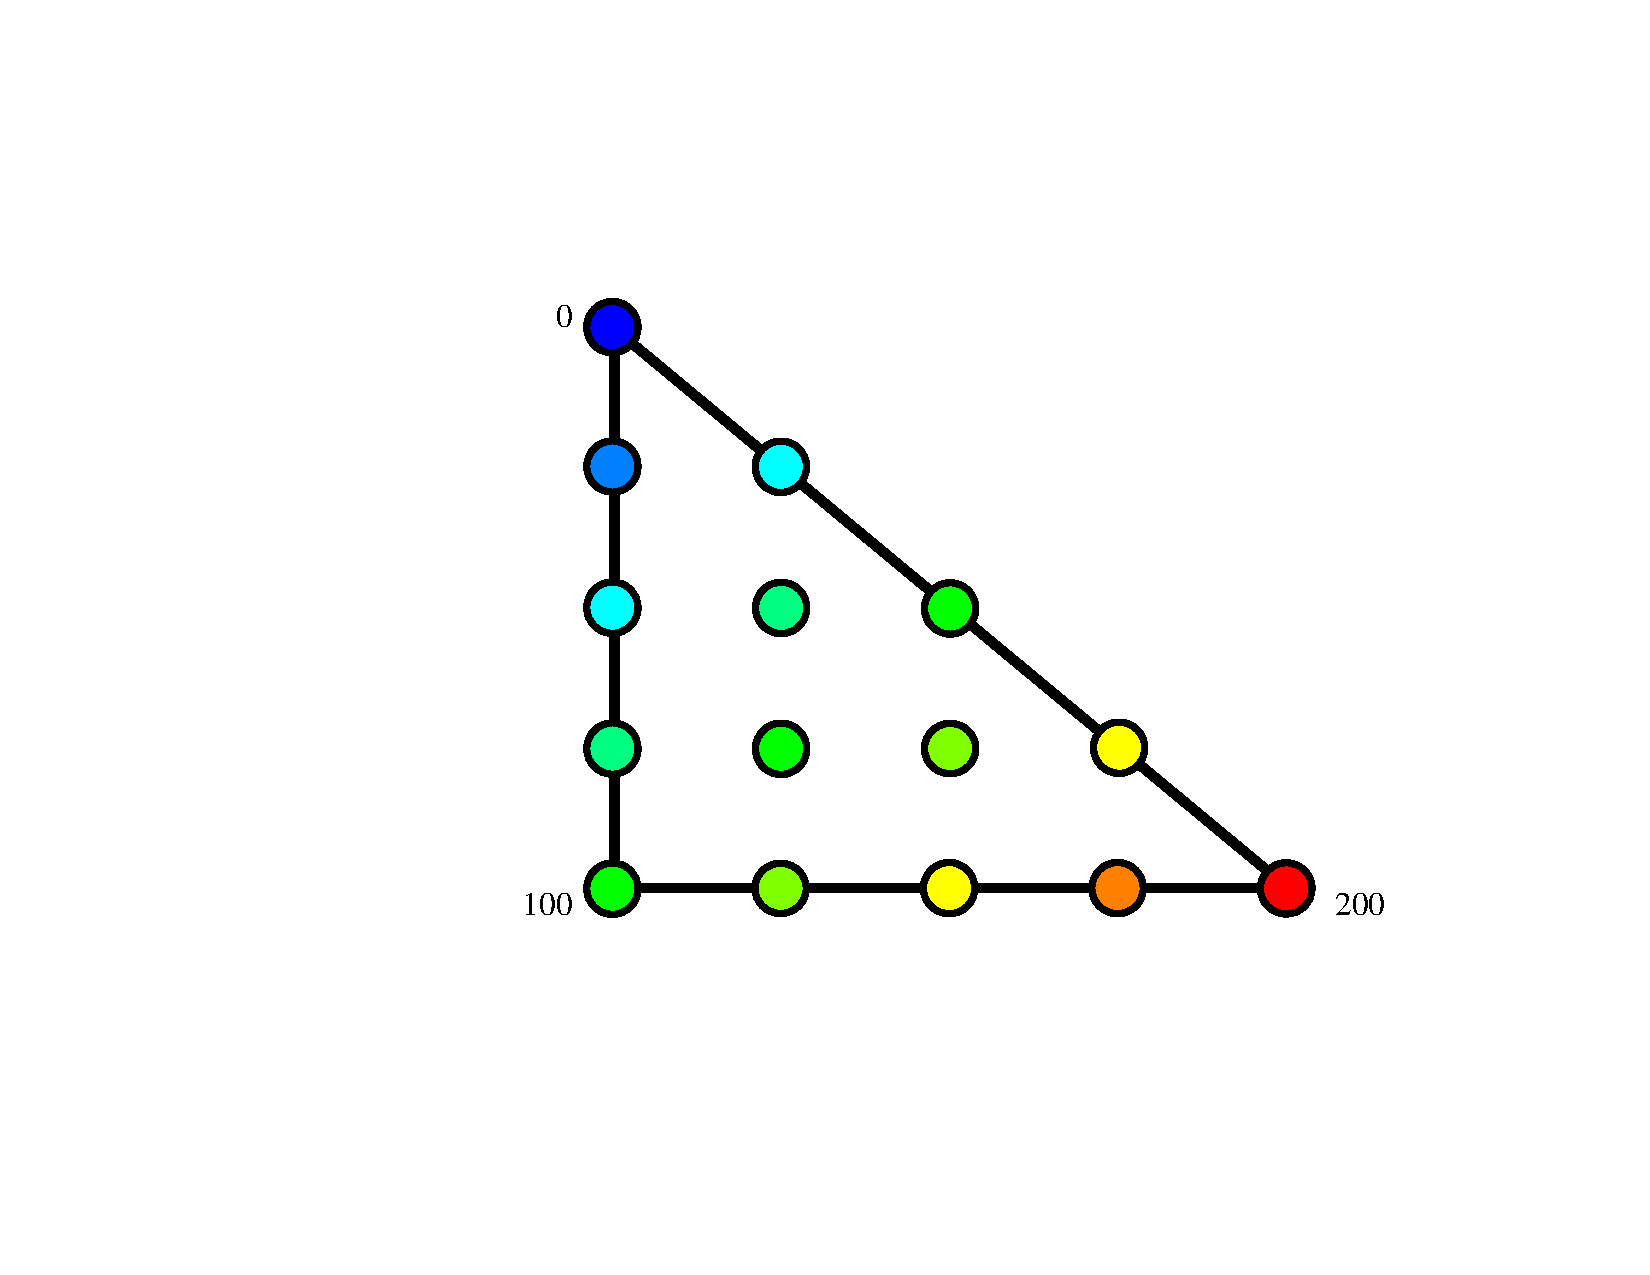
\includegraphics[height=4.0in]{\SMVfigdir/interpcolorindex}\\
b) colors interpolated within the colorbar\\
\end{tabular}
\end{center}
\caption[Color interpolation examples] {Illustration showing
colors representing data interpolated two different ways within a
triangle: interpolated with the 3D color cube and interpolated
with the colorbar}
\label{colorinterp}%
\end{figure}

%
% -------------------  2D Contours ------------------------
%

\section{2D Contours}

The {\em 2D contouring problem}\ may be stated as: find the region
in a 2D plane where a particular value exists {\em (line
contour)}\ or an interval of values exist {\em (banded contour)}.
In each case, the  region to be contoured is divided into a series
of squares.  The problem is solved for each square and assembled
to obtain the general solution.  The square locations correspond
to the grid set up in the FDS input file.

\subsection{Line contours}
\begin{figure}[bph]
\begin{center}
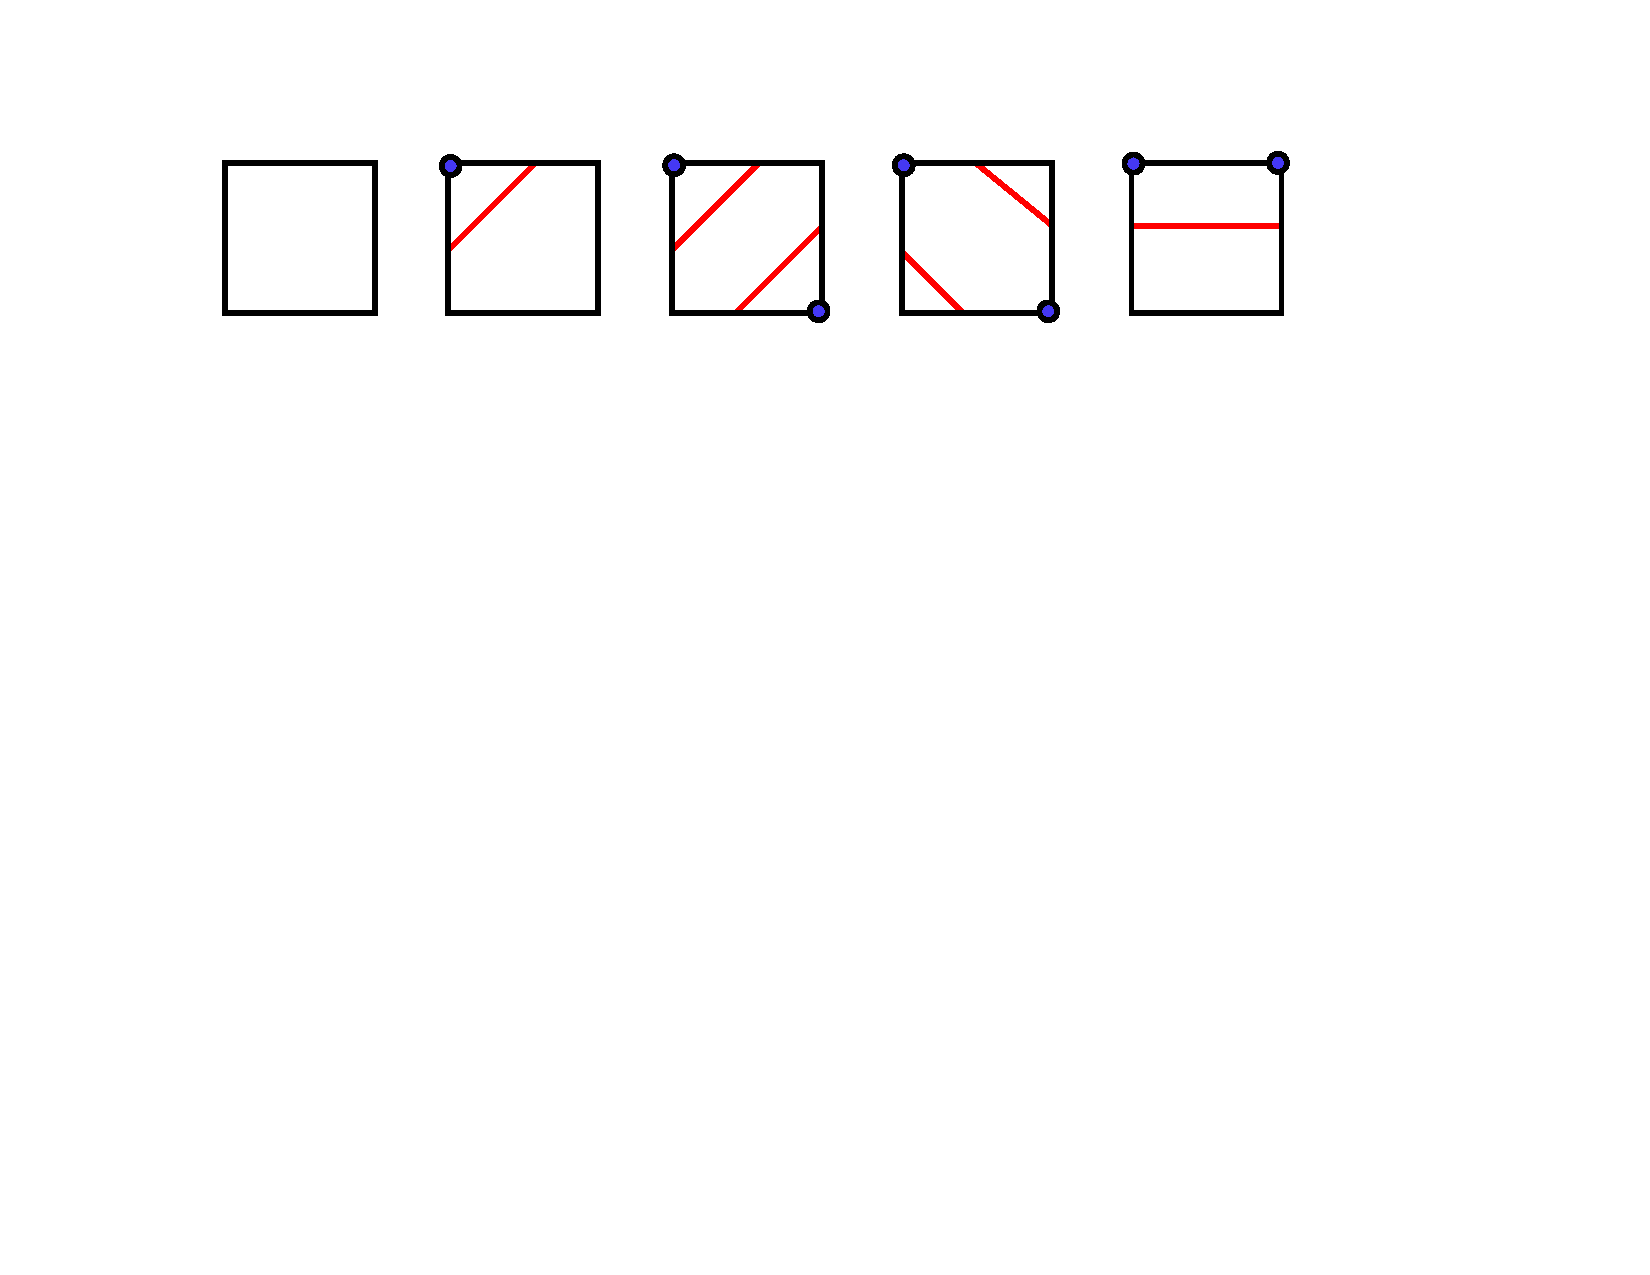
\includegraphics[width=7.0in]{\SMVfigdir/2d_linecontours}
\end{center}
\caption{2D line contour canonical forms.
  }
\label{fig2dline}%
\end{figure}
Mathematically, the 2D line contouring problem may be expressed
as: for some level $L$, find the line(s) in the desired region
where $f(x,y)=L$.  Consider this problem for one square and assume
that $f$ is known at each square corner.  The problem is solved by
noting that the value of $f$ at each of the four square corners is
either greater than or less than or equal to the contour level
$L$.  There are then two states at each of the four corners.  As a
result, there are 16 cases to consider.  These 16 cases may be
reduced to 4 after accounting for various symmetries such as
rotational, mirror and high/low.  High/low symmetry refers to the
observation that a case with one corner value above $L$ will look
the same as one with 3 corners above $L$. Figure \ref{fig2dline}
shows these four cases.  Corners with blue dots indicate that the
solution at this point is greater than $L$.  Red lines indicate
the line contouring solution.  The algorithm may be summarized as
follows:
\begin{enumerate}
\item Split the region to be contoured into a number of squares,
each square aligned with the underlying FDS grid.

\item For  each square:
\begin{enumerate}
\item Number the square corners as illustrated in Fig.
\ref{fig2dline}.

\item For each cell corner beginning with corner 0: assign 1 if
its value exceeds $L$, 0 otherwise.

\item Use resulting 4 digit binary number $(0\rightarrow 15)$ to
determine the case number to be plotted.  Using this numbering
scheme, the cases are numbered from left to right 0 1, 5 and 3.
\end{enumerate}
\end{enumerate}

\subsection{Banded contours}
\begin{figure}[bph]
\begin{center}
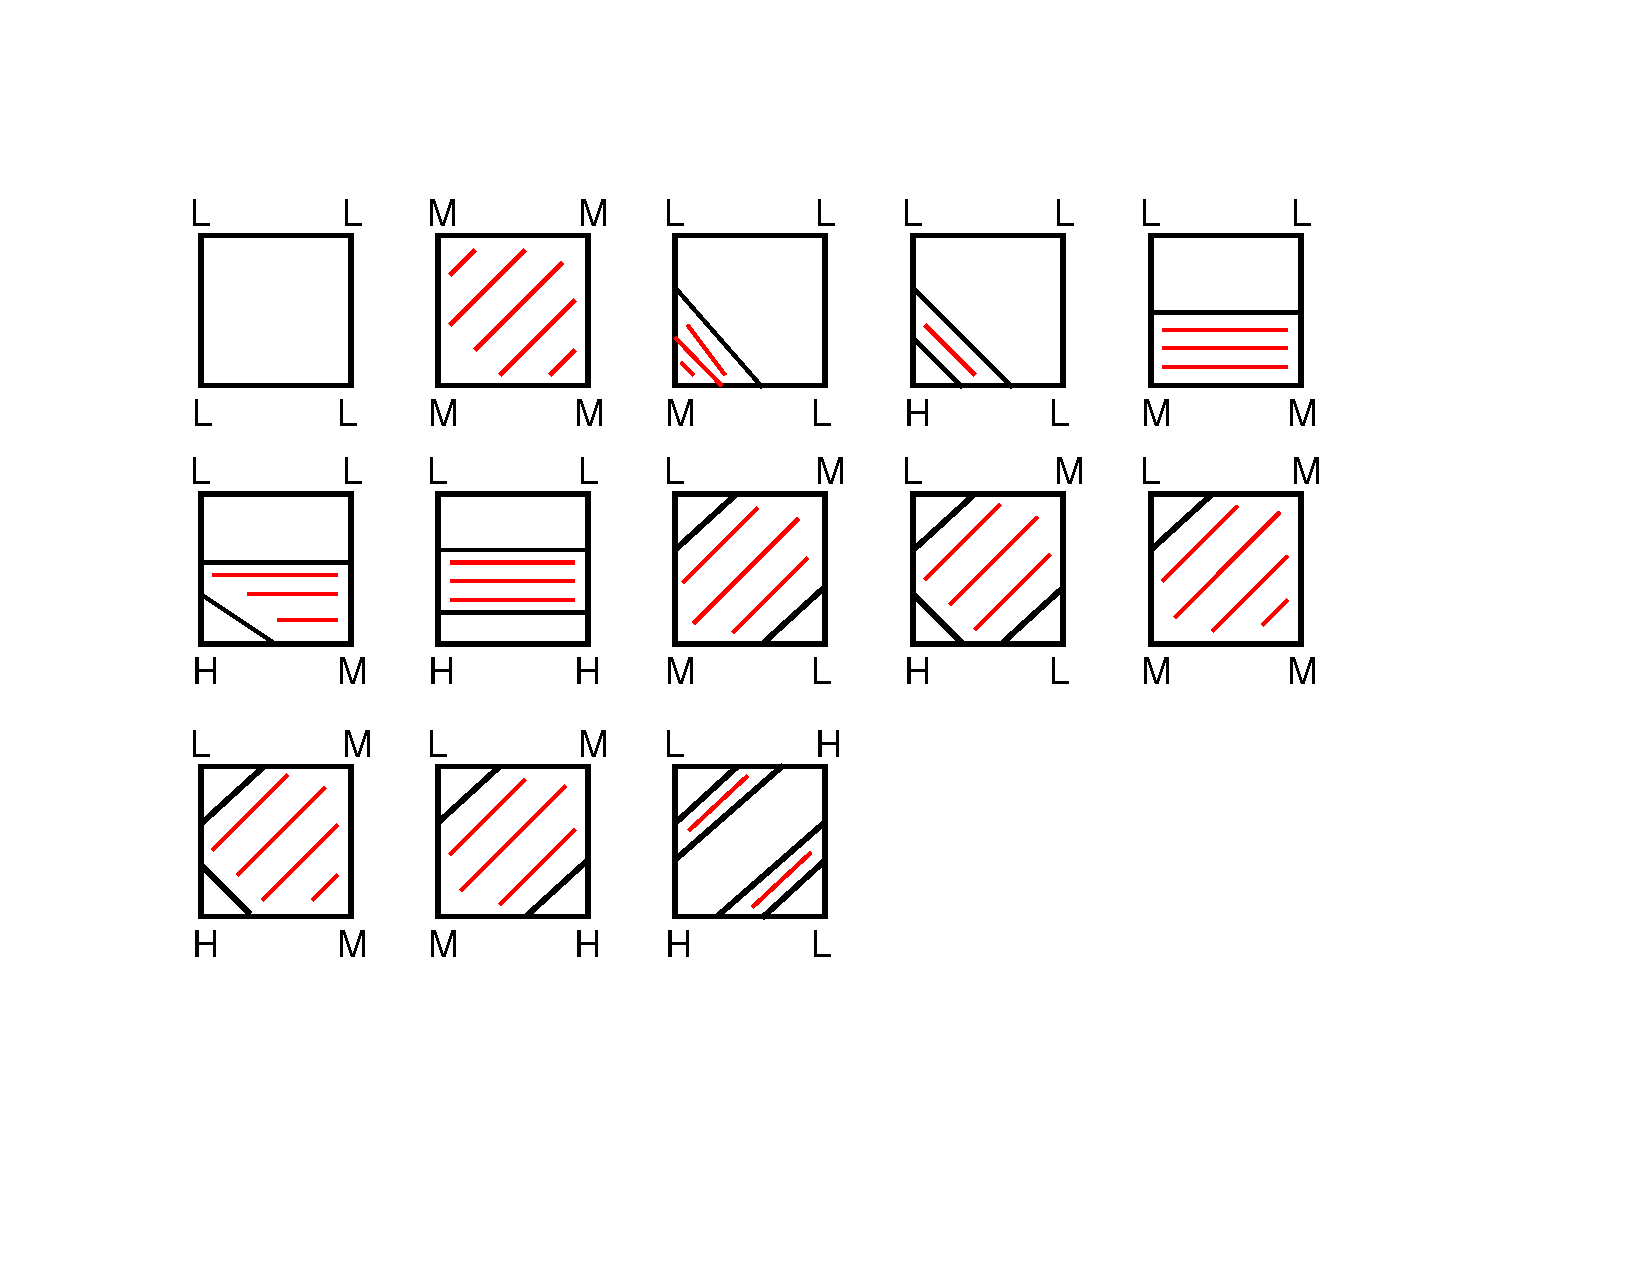
\includegraphics[width=7.0in]{\SMVfigdir/2d_bandcontours}
\end{center}
\caption{2D band contour canonical forms.
  }
\label{fig2dband}%
\end{figure}
The banded contouring algorithm works similarly to the line
contouring algorithm discussed previously.  The 2D banded
contouring problem may be expressed mathematically as given an
interval $[L,H]$, find the 2D region where $L\le f(x,y)\le H$. The
problem is solved by noting that the value of $f$ at each of four
square corners is either less than $L$, greater than $H$ or in
between.  There are three states at each of four corners resulting
in 81 cases to consider.  These 81 cases may be reduced to 13
after accounting for various symmetries such as rotational, mirror
and high/low. High/low symmetry is defined as before. Figure
\ref{fig2dband} shows these four cases.  Each square corner is
labeled with an L, M or H denoting that the value of $f$ at that
corner is below $L$, between $L$  and $H$ or above $H$
respectively.  The contoured region is bounded by black lines and
contains a series of one or more red lines in the interior. The
algorithm may be summarized as follows:
\begin{enumerate}
\item Split the region to be contoured into a number of squares,
each square aligned with the underlying FDS grid.

\item For  each square:
\begin{enumerate}
\item Number square corners as illustrated in Fig.
\ref{fig2dband}.

\item For each cell corner beginning with corner 0: assign 0 if
value is less than $L$, 1 if value is between $L$ and $H$ and 2 if
value exceeds $H$.

\item Use resulting 4 digit base 3 number $(0\rightarrow 80)$ to
determine the case number to be plotted. The case numbers in the
first row are 0, 40, 1, 2 and 3.  The case numbers in the second
row are 5, 8, 10, 11 and 13.  The case numbers in the last row are
14, 16 and 20.
\end{enumerate}
\end{enumerate}

%
% -------------------  3D Contours - Isosurfaces ------------------------
%

\clearpage
\section{3D Contours - Isosurfaces}
An isosurface is a surface in 3-D space that defines constant
values of a dependent variable. For example, if one is interested
in investigating regions at a certain temperature, say
\SI{100}{\degC}, one would generate an animated isosurface
specifying this value..

The isosurfaces are generated at each desired time step using a
marching cube algorithm~\cite{marchingcubes}\ modified to remove
ambiguities. A decimation procedure is used to reduce the number
of resulting triangles by collapsing nodes of triangles with large
aspect ratios and re-triangulating. This makes the isosurface look
better and also reduces storage requirements. Figures
\ref{figisoa} and \ref{figisob} illustrates the use of isosurfaces
for visualizing the stoichiometric mixture fraction. These figures
show different ways of drawing isosurfaces.

\paragraph{Isosurface uncertainty} Data used to generate isosurfaces
has uncertainty, therefore the location of the isosurface
also has uncertainty.  Bounds for this uncertainty may be expressed
in terms of data uncertainty and data variation (the smaller the
variation the larger the uncertainty).
The Smokeview verification guide~\cite{Smokeview_Verification_Guide}
shows that the uncertainty in isosurface location, $\Delta x$,
between two node, data value pairs $(x_1,T_1)$ and $(x_2,T_2)$  may be bounded using

\begin{eqnarray}
\left|\frac{\Delta x}{x_2-x_1}\right|\le \frac{\max(|\Delta
T_1|,|\Delta T_2|)}{|T_2-T_1|}
\end{eqnarray}

\noindent where $\Delta T_1$ and $\Delta T_2$ are the uncertainty
in $T_1$ and $T_2$ at $x_1$ and $x_2$ respectively.

\paragraph{Algorithm for generating an Isosurface} The algorithm for
generating an isosurface may be summarized as follows:
\begin{enumerate}
\item Split region to be contoured into a number of cubes, each cube
aligned with the underlying FDS grid.
\item For  each cube:
\begin{enumerate}
\item Number cube corners from 0 to 7 as illustrated in Fig.
\ref{figisosetup}. \item For each cube corner beginning with
corner 0: assign 1 if value exceeds $L$, 0 otherwise. \item Use
resulting 8 digit binary number $(0\rightarrow 255)$ to determine
the case number to be plotted. \item Triangulate cube surface,
storing vertex locations and edge numbers according to case
\end{enumerate}
\item Triangle decimation.  Eliminate small triangles (any
triangle with two or more vertices {\em closest}\ to the same
node). Replace removed triangle vertices with a vertex with
coordinates that are the average of the three removed vertices
coordinates.  Re-triangulate using this new vertex.  This process
is illustrated in Fig. \ref{figdecimate}. \item Estimate normal
directions (to be associated with a vertex).  For each vertex:
\begin{enumerate}
\item determine triangles sharing the vertex
\item determine the normal vector (normalized with length 1.0) of each
triangle using the vertex
\item construct a harmonic weighted average of triangle normal vectors
where all weights sum to 1.0 and each weight is inversely proportional
to the corresponding triangle area
\item store the resulting average along with vertex data
\end{enumerate}
\end{enumerate}

\paragraph{Vertex normals in 3D} An averaged normal vector, $V_i$, for
vertex $i$ may then be determined by summing over all triangles $n$
connected to a vertex $i$ as in
\begin{eqnarray}
V_{i}&=&\sum_n\frac{U_n}{A_n}/\sum_n\frac{1}{A_n}
=\sum_n\frac{u_n\times v_n}{||u_n\times
v_n||^2}/\sum_n\frac{1}{||u_n\times v_n||}
\end{eqnarray}
where for the $n$'th triangle, $u_n$ and $v_n$ are two sides,
$A_n=||u_n\times v_n||$ is the triangle area and $U_n=u_n\times v_n/A_n$
is a unit vector normal to the triangle.


\begin{figure}[bph]
\begin{center}
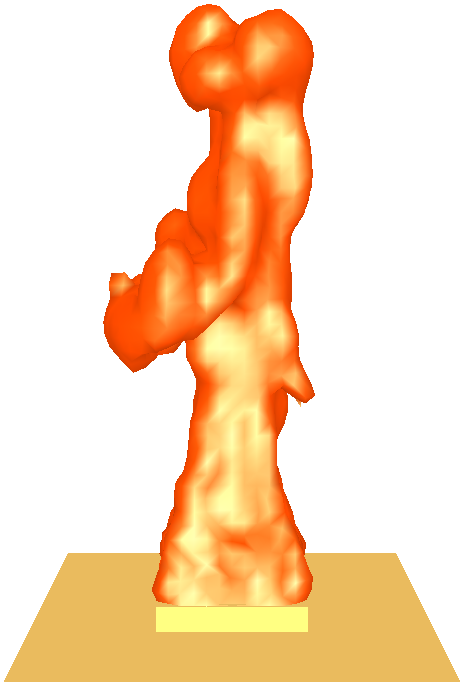
\includegraphics[height=8.5in]{\SMVfigdir/plume5a_iso_full}\\
\end{center}
\caption{Snapshot of an isosurface of temperature at 100 \degC\ (212 \degF).
  }
\label{figisoa}%
\end{figure}

\begin{figure}[bph]
\begin{center}
\begin{tabular}{c}
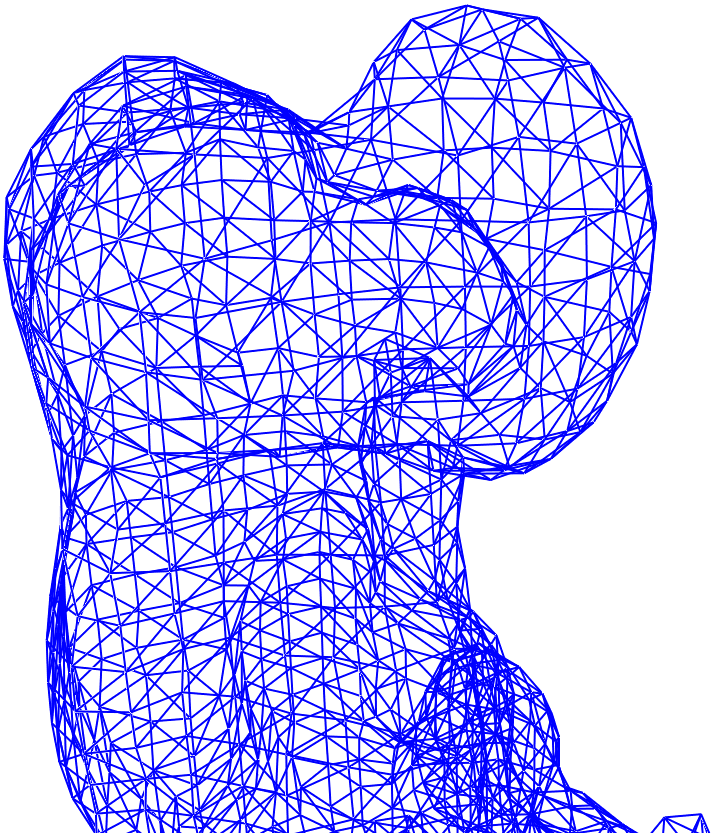
\includegraphics[height=4.0in]{\SMVfigdir/plume5a_iso_lines}\\
outline view\\
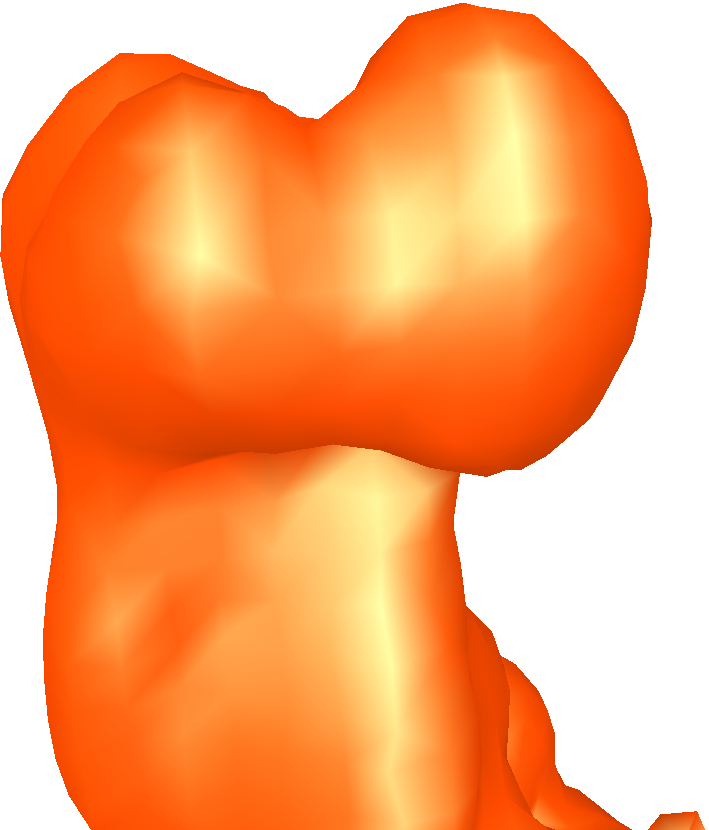
\includegraphics[height=4.0in]{\SMVfigdir/plume5a_iso_solid}\\
solid view
\end{tabular}
\end{center}
\caption{Snapshot of an isosurface of temperature at 100 \degC\ (212 \degF).
  }
\label{figisob}%
\end{figure}

\begin{figure}[bph]
\begin{center}
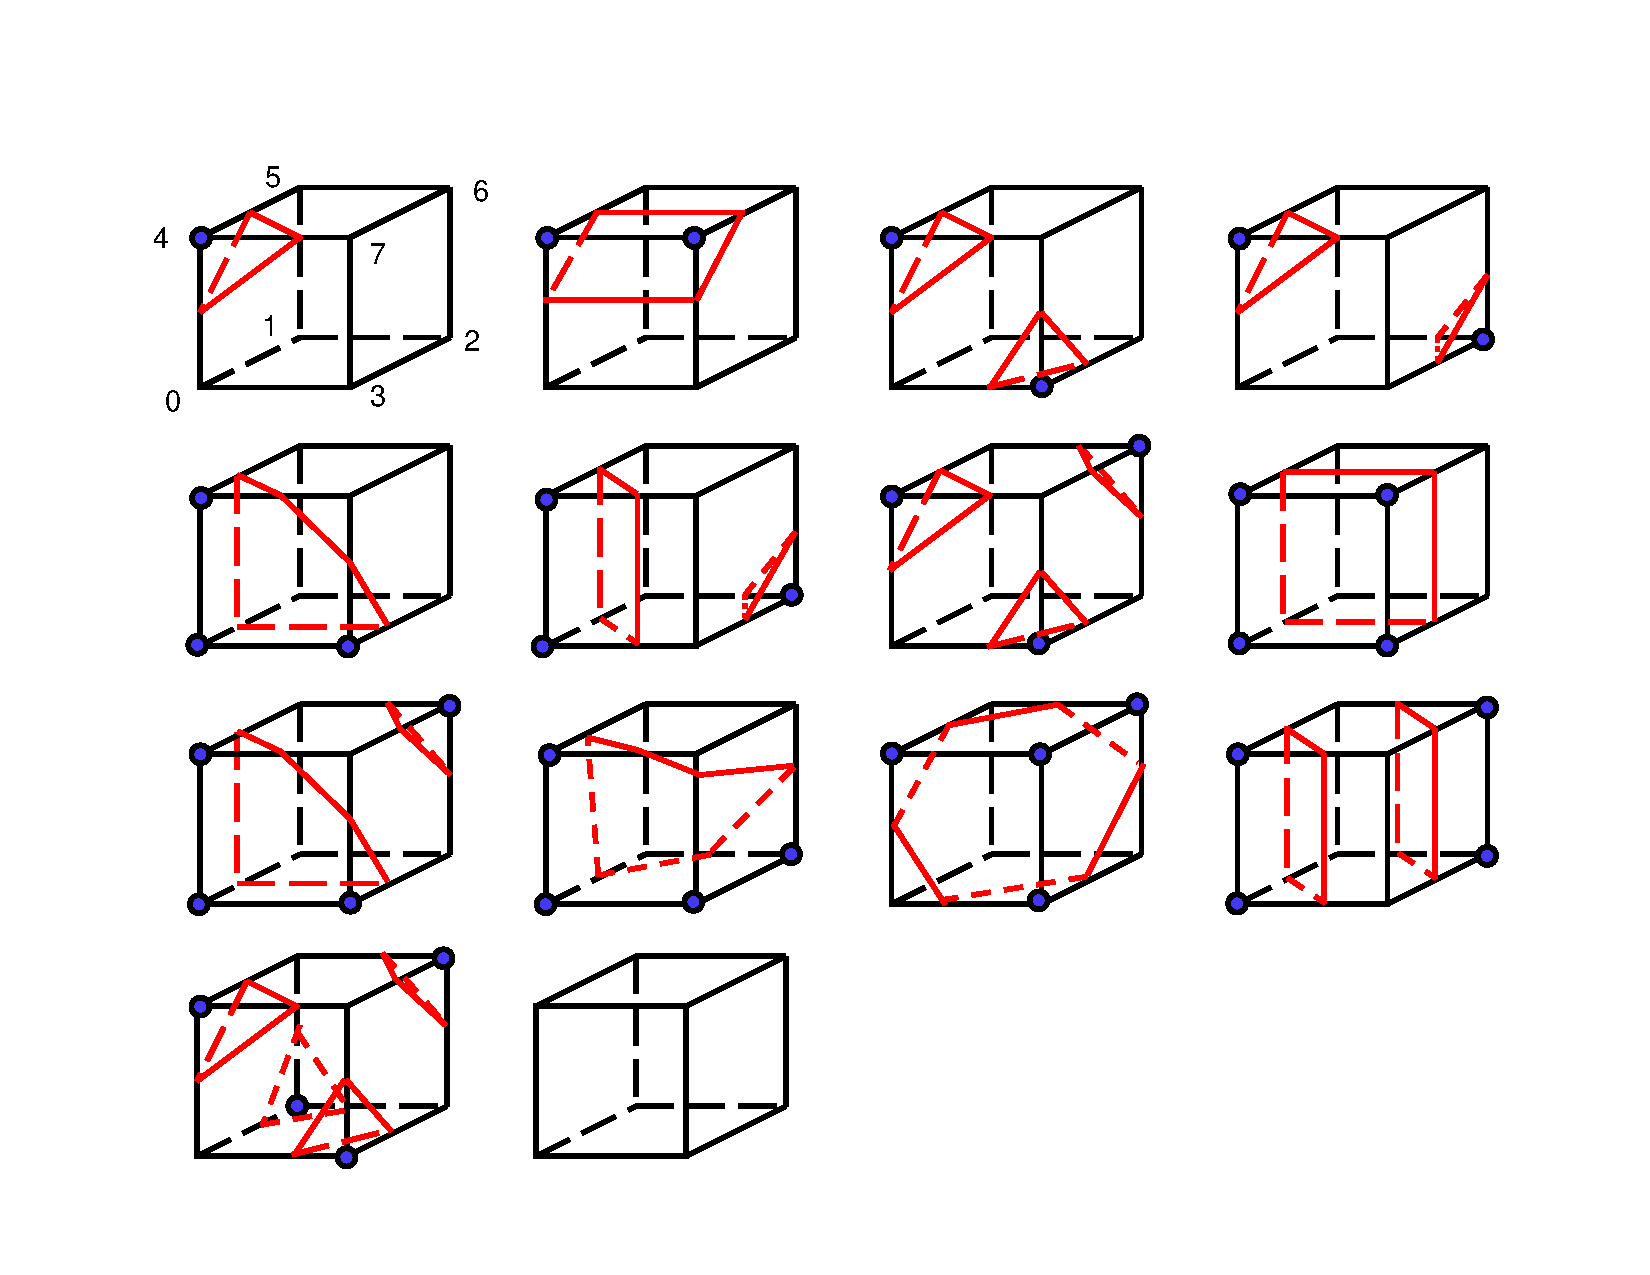
\includegraphics[width=7.0in]{\SMVfigdir/3d_contours}
\end{center}
\caption[3D isosurface canonical forms.]{3D isosurface canonical
forms. Dots occur at corners where the data value is greater than
the isosurface value.  Other corners are below the isosurface
value.  Red polygons intersect cube edges at the isosurface value.
The red polygon (isosurface) NEVER intersects an edge with two or
zero dots on the ends.
  }
\label{figisosetup}%
\end{figure}


\begin{figure}[bph]
\begin{center}
\begin{tabular}{c}
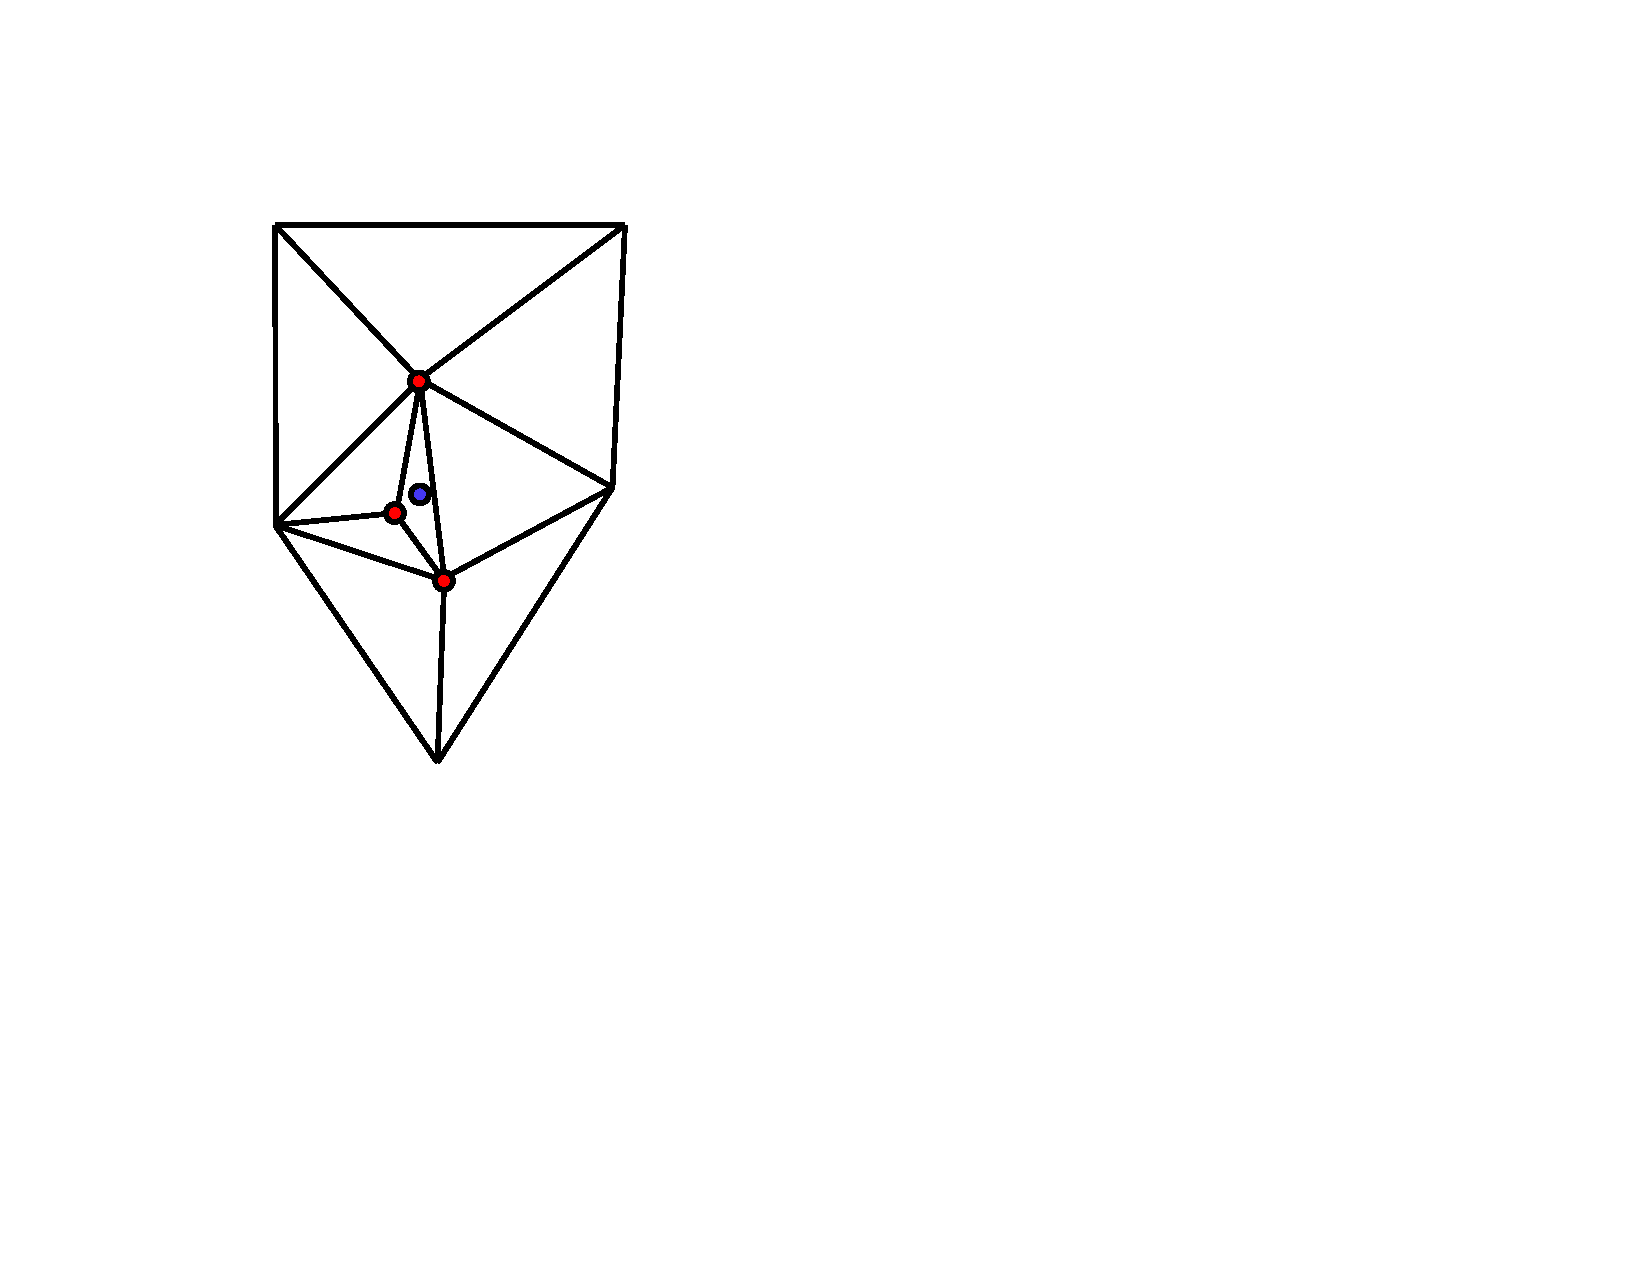
\includegraphics[height=4.0in]{\SMVfigdir/decimate_before}\\
before decimation\\
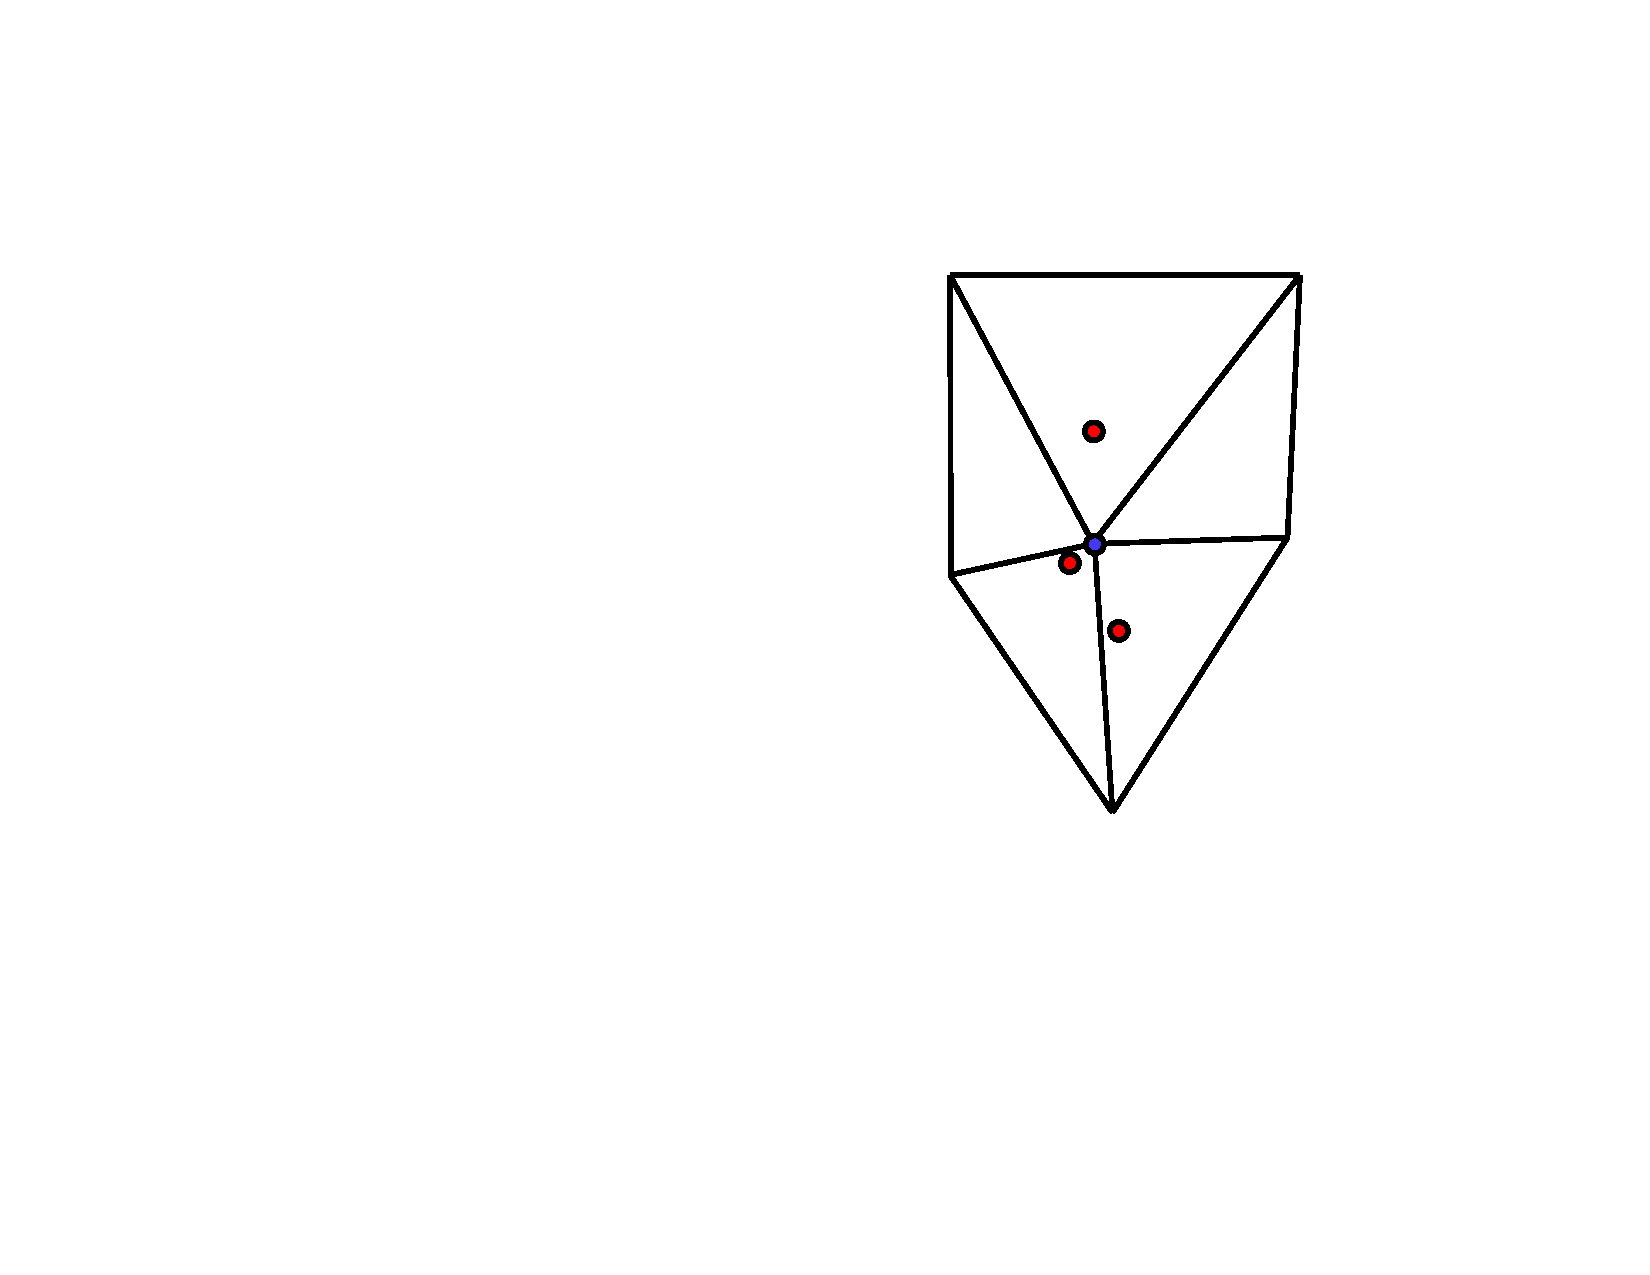
\includegraphics[height=4.0in]{\SMVfigdir/decimate_after}\\
after decimation
\end{tabular}
\end{center}
\caption[Example of triangle decimation.]{Example of triangle decimation.
Triangle with red dots is removed.  Region is re-triangulated by replacing
any edges connected to a red dot with the blue dot (average position of removed red dot).}
\label{figdecimate}%
\end{figure}

%
% -------------------  Section on isosurface slope derivation ------------------------
%

\begin{figure}[bph]
\begin{center}
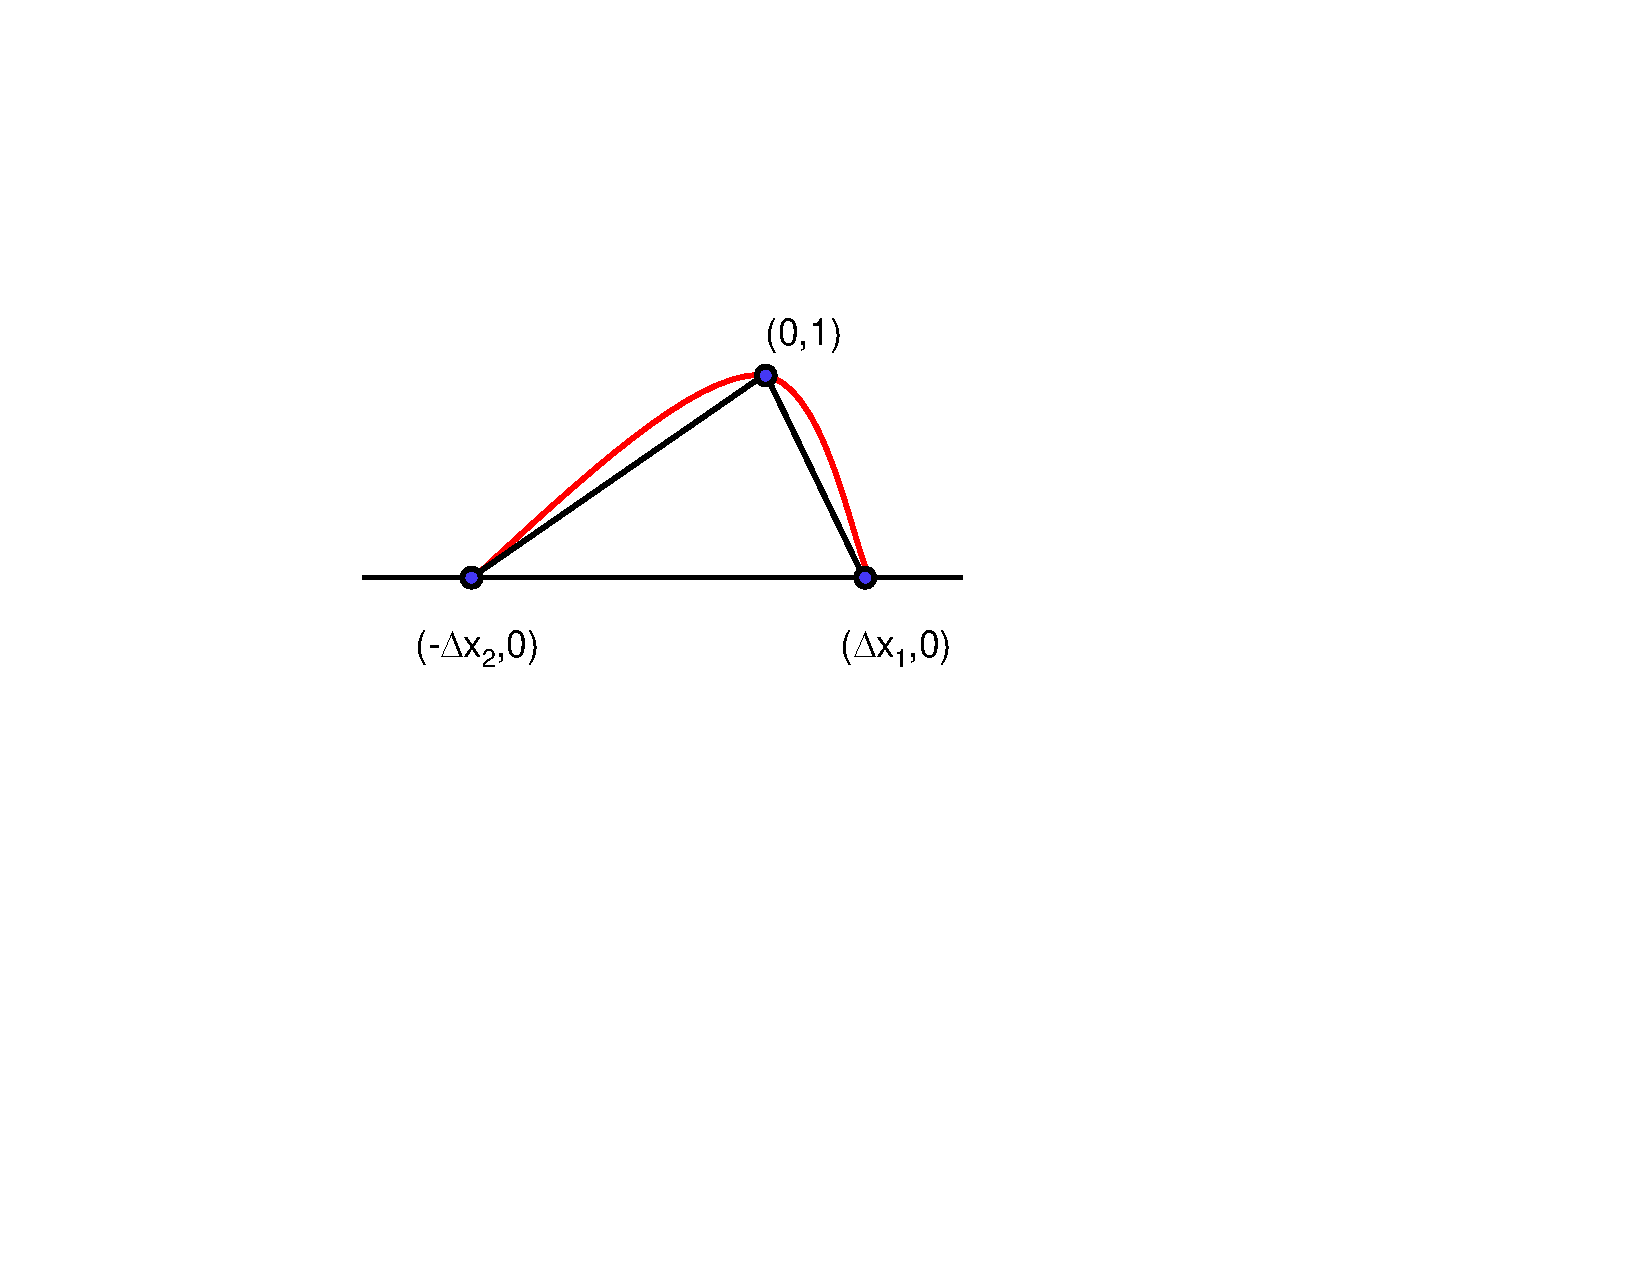
\includegraphics[width=5.0in]{\SMVfigdir/3point_line_smooth}
\end{center}
\caption{Setup for determining the slope of a smooth curve passing through three points.}
\label{figlinesmooth}%
\end{figure}

\paragraph{Vertex normals in 2D} The use of inverse area weights or
harmonic averages to construct average normal vectors at isosurface
vertices is justified by the following two dimensional example.
As illustrated in Fig. \ref{figlinesmooth}, consider the
quadratic $y(x)=A+Bx+Cx^2$ with $y(-\Delta x_2)=0$,
$y(0)=1$ and $y(\Delta x_1)=0$ .  The slope at $x=0$ is given by $y'(0)=B$.
Likewise, the slope of the vector perpendicular to this curve at $x=0$ is $-1/B$.
The coefficient $B$ may be determined from the two simultaneous equations
$y(\Delta x_1)=0$ and  $(y(-\Delta x_2)=0$ (note that $A=1$ since $y(0)=1$) or
\begin{eqnarray}
1+B\Delta x_1 + C \Delta x_1^2 &= &0\\
1-B\Delta x_2 + C \Delta x_2^2 &= &0
\end{eqnarray}
which has solution
\begin{eqnarray}
B&=&\frac{\Delta x_1^2-\Delta x_2^2}{\Delta x_1\Delta x_2(\Delta x_1+\Delta x_2)}=
\frac{\Delta x_1-\Delta x_2}{\Delta x_1\Delta x_2}
\end{eqnarray}
The slope $N$ of the normal at $x=0$ is then given by
\begin{eqnarray}
N=-\frac{1}{B}&=&\frac{1}{1/\Delta x_1-1/\Delta x_2}
\end{eqnarray}
The slope $N_1$ of the normal to the line segment between
$(0,1)$ and $(\Delta x_1,0)$ is $N_1=\Delta x_1$.
The slope $N_2$ of the normal to the line segment between
$(-\Delta x_2,0)$ and (0,1) is $N_2=-\Delta x_2$.
Therefore the average slope $N$ may be expressed in terms of
$N_1$ and $N_2$ as
\begin{eqnarray}
N=\frac{1}{1/N_1+1/N_2}
\end{eqnarray}

\paragraph{Isosurface opacity}Consider a portion of an isosurface oriented at an angle $\theta$ from
the observer,as illustrated in Figure \ref{fig:isosetup}.  The vector $\vec{n}$ represents the direction
perpendicular from the surface and the vector $\vec{v}$ represents the direction from the surface to the observer.
The distance $\Delta\hat{x}$ through the surface from the point of view
of the observer is then given by
\begin{equation}
\frac{\Delta \hat{x}}{\Delta x}=\frac{1}{\cos\theta}=
\frac{||\vec{n}||~||v||}{\vec{n}\cdot\vec{v}}
\end{equation}
\noindent where $\theta$ is the angle between $\vec{n}$ and $\vec{v}$.
Let $\alpha=1-\exp(A\Delta x)$ represent the opacity corresponding to
a surface thicness $\Delta x$.  Then the opacity when the surface is
oriented an angle $\theta$ with resepect to the observer is given by
\begin{eqnarray*}
\hat{\alpha}&=&1-e^{A\Delta\hat{x}}\\
&=&1-(e^{A\Delta x})^\frac{\Delta \hat{x}}{\Delta x}\\
&=&1-(1-\alpha)^\frac{\Delta\hat{x}}{\Delta x}\\
&=&1-(1-\alpha)^\frac{||\vec{n}||~||\vec{v}||}{\vec{n}\cdot\vec{v}}
\end{eqnarray*}


\begin{figure}[bph]
\begin{center}
\includegraphics[width=5.0in]{\SMVfigdir/iso_setup}
\end{center}
\caption[Setup for determining isosurface opacity as a function of orientation.]
{Setup for determining isosurface opacity as a function of orientation.
The vectors $\vec{n}$ and $\vec{v}$ represent the direction perpendicular to the surface
and the direction from the surface to the observer.}

\label{fig:isosetup}%
\end{figure}

Figure \ref{fig:isoexample} shows an example of an isosurface using this equation for modeling opacity.

\begin{figure}[bph]
\begin{center}
\includegraphics[width=5.0in]{../SMV_Verification_Guide/SCRIPT_FIGURES/plume5c_iso_solid_30}
\end{center}
\caption
{Isosurface with variable opacity. The isosurface opacity changes as a function of orienttion
with repsect to the observer.}

\label{fig:isoexample}%
\end{figure}


\section{Particle Systems}
\subsection{Massless Particles}
FDS uses particles as tracer elements to allow one to visualize
flow.  FDS also uses particles as droplets to model fire
suppression or as fuel elements that can be transported and
burned, for example, as embers emitted from a burning tree.
Particle positions are determined in FDS using the differential
equation
\begin{eqnarray}
\frac{dx_p}{dt}=V(x_p,t)
\end{eqnarray}
where $x_p$ represents particle position and $V$ represents the
velocity field.

The assumption this model uses to compute particle flow is that
the drag force on the particle is large compared to $mg$, the
force due to gravity.

Figure \ref{figpart} shows particles represented as particles and
as streaks. A particle streak visualizes where a particle is
located over a period of time.  The streak length is specified as
time. Static particle images are not effective at displaying
motion.  For example, the particle image in Fig. \ref{figpart}a
does not show particle motion.  Streak lines, however, in Fig.
\ref{figpart}b shows curved motion due to interior obstructions.
Particle size is specified using
\begin{lstlisting}
glPointSize(partpointsize);
\end{lstlisting}
The floating point value of {\tt partpointsize}\ is specified
using the {\tt File/Bounds} dialog box.  Streak line length is
specified in terms of time, a certain number of seconds before the
current display time.  Streak length is also specified in the {\tt
File/Bounds}\ dialog box.

\begin{figure}[bph]
\begin{center}
\begin{tabular}{cc}
\includegraphics[width=3.0in]{../SMV_Verification_Guide/SCRIPT_FIGURES/plume5c_part}&
\includegraphics[width=3.0in]{../SMV_Verification_Guide/SCRIPT_FIGURES/plume5c_streak}\\
a) Particles&b) Particle streaks\\
\end{tabular}
\end{center}
\caption{Plume flow visualized using particles and particle streaks.}
\label{figpart}%
\end{figure}

\section{Computing and Visualizing Fractional Effective Dose data}
The fractional effective dose (FED), developed by
Purser~\cite{SFPE:Purser}, is a measure of human incapacitation
due to combustion gases.  FED index data is computed by Smokeview
using CO, $\mathrm{CO_2}$ and $\mathrm{O_2}$ gas concentration
data computed by FDS. Future work involves incorporating other
constituents such as soot or HCN.  Smokeview obtains this data
from FDS using slice files.

The total FED is computed here in terms of FED components for CO
and $\mathrm{O_2}$.  A hyper-ventilating factor due to
$\mathrm{CO_2}$ is applied to the FED for CO. The total FED is
then given by

\be \mathrm{FED}_\mathrm{tot} = \mathrm{FED}_\mathrm{CO} \times
\mathrm{HV}_\mathrm{CO_2} + \mathrm{FED}_\mathrm{O_2} \ee

Other terms involving CN, NOx and irritants are neglected. The
fraction of an incapacitating dose due to CO,
$\mathrm{FED}_\mathrm{CO}$ is calculated using

\be \mathrm{FED}_\mathrm{CO}(t) = \int_0^t 2.764 \times 10^{-5} \,
(C_\mathrm{CO}(t))^{1.036} \, dt \label{eq:fedCO} \ee

where $t$ is time in minutes and $C_\mathrm{CO}$ is the CO
concentration (ppm). The fraction of an incapacitating dose due to
low O${}_2$ hypoxia , $\mathrm{FED}_\mathrm{O_2}$, is calculated
using

\be \mathrm{FED}_\mathrm{O_2}(t) =  \int_0^t \frac{dt}{\exp \left
[ 8.13 - 0.54 \, (20.9 - C_\mathrm{O_2}(t)) \right ] }
\label{eq:fedO2} \ee

where $t$ is time in minutes and $C_\mathrm{O_2}$ is the O${}_2$
concentration (volume per cent). The hyperventilation factor
induced by carbon dioxide, $\mathrm{HV}_\mathrm{CO_2}$, is
calculated using

\be \mathrm{HV}_\mathrm{CO_2}(t) = \frac{ \exp( 0.1903 \,
C_\mathrm{CO_2}(t) +  2.0004 ) }{7.1} \label{eq:co2hyp} \ee

where $t$ is time in minutes and $C_\mathrm{CO_2}$ is the
$\mathrm{CO_2}$ concentration (percent).

\subsection{FED example}
Assuming that $C_\mathrm{CO}(t)=\mathrm{CO}$,
$C_\mathrm{CO_2}(t)=\mathrm{CO_2}$ and
$C_\mathrm{O_2}(t)=\mathrm{O_2}$ are constant, equations
\ref{eq:fedCO}, \ref{eq:fedO2} and \ref{eq:co2hyp} reduce to

\be \mathrm{FED}_\mathrm{CO}(t) = 2.764 \times 10^{-5} \,
\mathrm{CO}^{1.036} \, t \label{eq:fedCOcons} \ee

\be \mathrm{FED}_\mathrm{O_2}(t) =   \exp( -8.13 + 0.54 \, (20.9 -
\mathrm{O_2}) )t \label{eq:fedO2cons} \ee

\be
\mathrm{HV}_\mathrm{CO_2}(t) = \frac{ \exp( 0.1903 \, \mathrm{CO_2} +  2.0004 ) }{7.1}
\label{eq:fedCO2cons}
\ee

so that the total FED is given by

\begin{eqnarray}
\mathrm{FED}_\mathrm{tot}
&= &\mathrm{FED}_\mathrm{CO}(t)\times\mathrm{HV}_\mathrm{CO_2}(t)+\mathrm{FED}_\mathrm{O_2}(t)\\
\nonumber
 &= &\left(2.764 \times 10^{-5} \, \mathrm{CO}^{1.036}\times
\frac{ \exp( 0.1903 \, \mathrm{CO_2} +  2.0004 ) }{7.1} + \exp( -8.13
+ 0.54 \, (20.9 - \mathrm{O_2}) )\right) t\\
\end{eqnarray}

Figure \ref{fig:fedplot} presents two FED computations where CO,
$\mathrm{CO_2}$ and $\mathrm{O_2}$ are constant.
The first for a smoke filled room with CO=\SI{10000}{ppm},
$\mathrm{CO_2}=5 \%$ and $\mathrm{O_2}=10 \%$ and the second for a
room with ambient conditions with CO=\SI{0}{ppm},
$\mathrm{CO_2}=0.04 \%$ and $\mathrm{O_2}=21 \%$

\begin{figure}[bph]
\begin{center}
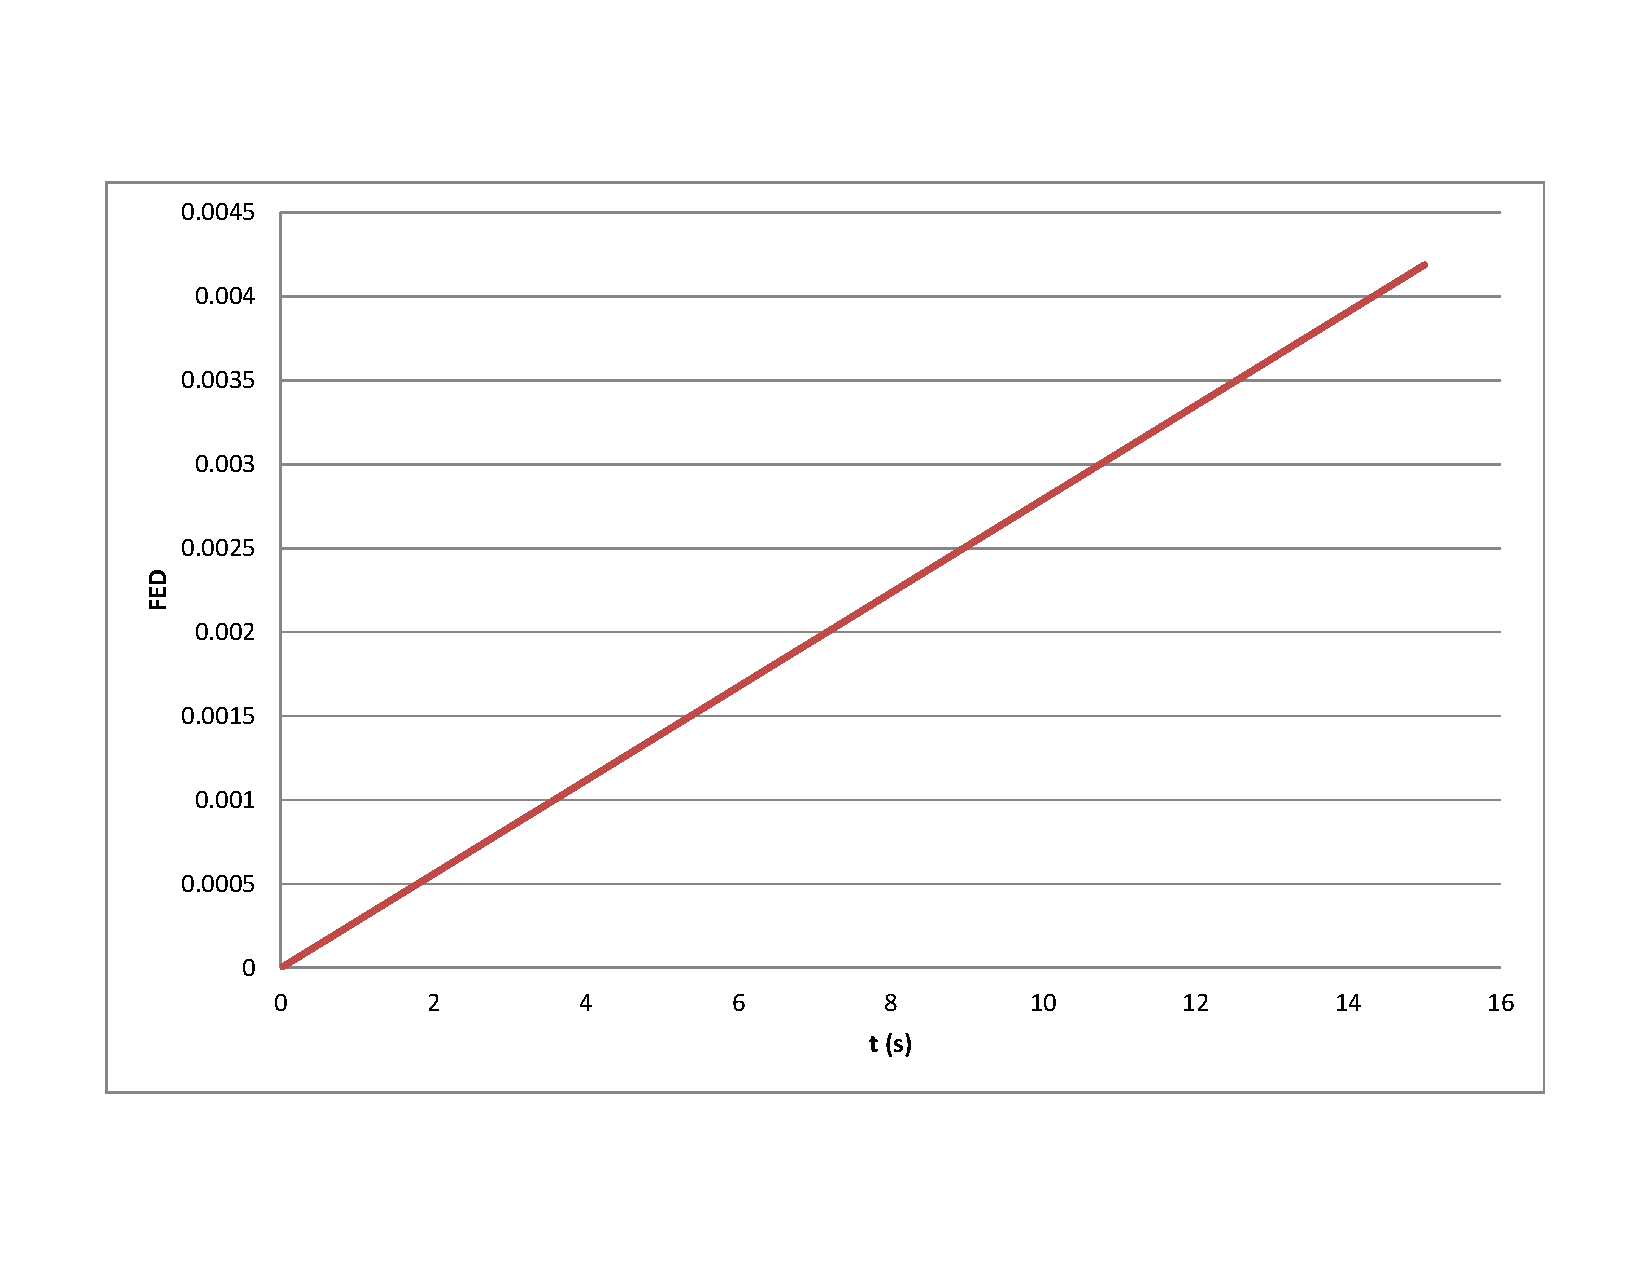
\includegraphics[width=5.0in]{\SMVfigdir/fed_clear}\\
a) ambient\\
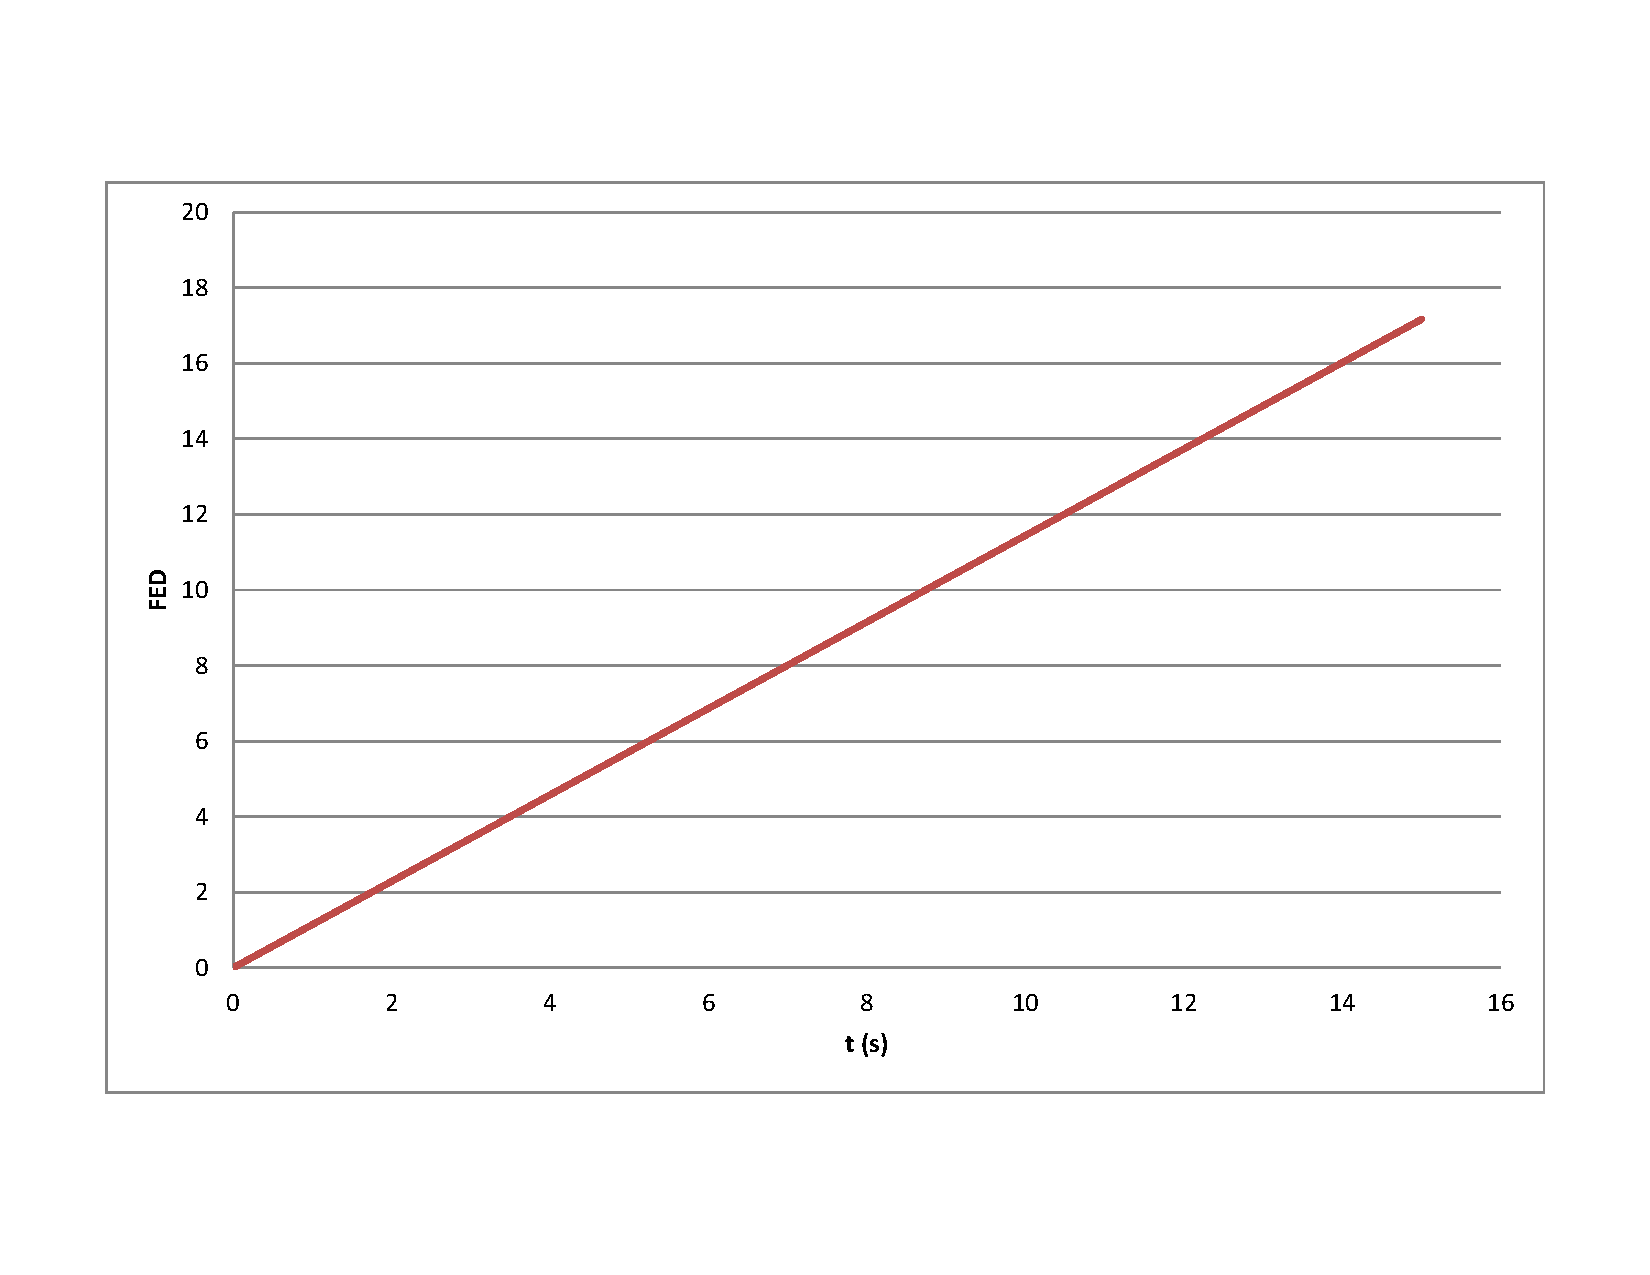
\includegraphics[width=5.0in]{\SMVfigdir/fed_smoke}\\
b) smoke filled
\end{center}
\caption{Plot of FED vs. time for ambient and smoke filled rooms.}
\label{fig:fedplot}%
\end{figure}

%
% -------------------  Volumetric Methods ------------------------
%

\chapter{Visualizing Smoke and Fire}

\newcommand{\citesmv}{\cite{Smokeview_Users_Guide}}
\newcommand{\paper}{chapter}
% $Date$
% $Revision$
% $Author$

% !TEX root = SMV_Technical_Reference_Guide.tex

% -------------------  Introduction ------------------------

\section{Introduction}
This \paper\ documents the physics and associated numerical
algorithms used by Smokeview~\cite{Smokeview_Users_Guide} to
visualize smoke and fire.  Smoke color and opacity are visualized
using quantitative physics based methods.  Flame color at present
is visualized using an arbitrary user specified color palette
where color is mapped to gas temperature. Future work involves
mapping color to a blackbody temperature curve enabling a more
quantitative choice of color for this application.

Realistic visualization of fire calculation methods are important
for applications where one wishes to observe qualitative effects
of fire and smoke rather than determine quantitative
characteristics of data such as temperature or velocity.  This
would be the case for a fire fighter using a computer based fire
fighting simulator. Realistic visualization methods, however,
complement but do not replace other more traditional visualization
methods such as 2D contouring or 3D iso-surfacing which are better
suited for quantitatively analyzing data.

Complete methods for visualizing smoke and fire data taking into
account interactions between light and smoke require the solution
of the radiation transport equation (RTE)~\cite{Siegel:2001} also
called the volume rendering equation in visualization
literature.~\cite{levoy:1988} This equation models how light is
affected after interacting with smoke, a participating medium. In
particular, Smokeview uses the RTE to account for extinction
(absorption plus out-scattering) by the smoke and emission from
the fire.

The form of the RTE used by Smokeview to model smoke and fire
appearance is identical to that used by FDS to model radiative
heat transfer. Smokeview uses an extinction coefficient
appropriate for visible light while FDS use one appropriate for
infrared wavelengths of light.  With the proper extinction
coefficient, however, Smokeview can also view smoke at other
wavelengths, simulating a thermal imager, for example. Smokeview
solves the RTE assuming a gray gas environment. This is the
default solution method for FDS. One other important difference is
that Smokeview requires a solution at only one point at a time
(any arbitrary point though), the observer's viewpoint, while FDS
requires a radiation field, a solution at all points within the
solution domain.  Even so, the solution of this
integro-differential equation for visualization requires
significant computation and memory  resources. Approximations are
required in order to display smoke and fire at interactive frame
rates.  The primary approximation is to take advantage of the low
albedo character of smoke allowing one to either simplify or
eliminate scattering terms in the RTE.

Two techniques discussed for visualizing smoke are slice rendered
and volume rendered methods~\cite{levoy:1988,Engel:2006}.    These
methods both solve a form of the RTE equation.  The integrated
quantity in both cases is radiance, the intensity of light seen by
the observer.  They differ in how the integration path is
partitioned.

The first approach, a slice rendering method,  splits the
integration path at grid planes within a 3D mesh. There is one
partially transparent slice for each plane of simulated data.
Planes are drawn through the data along the coordinate planes or
diagonally to these  planes.   The particular plane drawn is
chosen to be the one most perpendicular to the viewer's line of
sight.  The resulting partially transparent slice planes are drawn
individually and combined by the video hardware to form one image.

The separation distance between slice planes becomes smaller as
more planes are used to simulate a case.  As a result, the
computed opacity values are subject to increased round off error
due to finite precision arithmetic.  In fact, if these planes are
sufficiently close, the computed opacities truncate to zero.   In
this situation, volume rendering methods are required.

The second approach, a volume rendering method, also integrates a
simplified form of the radiation transport equation, but over the
entire data mesh.  The integration occurs from the front of the
solution domain (relative to the observer) to the back, rather
than across just one slice plane. By performing the entire
integral at once instead of in pieces, the volume rendered method
does not suffer from the round off errors of the slice rendered
method.  The intermediate computational terms in the volume
rendered method are stored using full precision arithmetic rather
than 8 bits.  A volume rendered method then computes opacity
across multiple grid planes.  As a result, there is only one plane
of data displayed.  The video hardware is again exploited, but
this time to compute a line integral for each pixel in the
observer's view.  Opacities and color for both methods are
computed using transfer functions using soot density and
temperature data obtained from a fire simulation.

This \paper\ is organized as follows.  A model for visualizing
smoke and fire is discussed.  This model, the radiative transport
equation (RTE), is simplified in several ways, one of which gives
the Beer-Lambert law.  Two methods are then discussed for
visualizing smoke  both using a form of the RTE.  The first
method, slice rendering,  uses a series of partially transparent
slices to represent smoke and fire. The second method, volume
rendering, solves the RTE over the entire domain. Finally, several
areas for which the visualization methods may be improved are
given.

% -------------------  Radiation Transport Equation ------------------------

\section{Radiation Transport Equation}
The model used here to visualize smoke is the radiation transport
equation (RTE)~\cite{Siegel:2001}.  This equation uses radiance to
represent smoke appearance.  Radiance has units of Watts per
square meter per unit solid angle~\si{W/(sr.m^2)}.  The solid
angle accounts for the fact that a light source appears brighter
if it emits a given amount of light through a smaller
cross-sectional area.  This has the interesting implication,
ignoring atmospheric effects and as pointed out in
Ref.~\cite{dutre:2002}, that the sun's radiance appears the same
observed from Earth as from Mars.  The diminished heat flux
\si{(W/m^2} on Mars due to the increased distance from the
sun is exactly offset by the reduced solid angle (\si{sr}) that the
sun's disk subtends.  From a visualization perspective, this
implies that image radiance does not depend on distance from the
observer unless  a participating medium is present to absorb or
scatter  light.  The radiation transport equation discussed in
this section models the change in radiance due to these factors.

\renewcommand{\dx}[1]{\,\mbox{d}#1}
\newcommand{\siga}{ \sigma_a(x) }
\newcommand{\sigt}{ \sigma_t(x) }
\newcommand{\sigs}{ \sigma_s(x) }
\newcommand{\sigts}{ \sigma_t(s) }
\newcommand{\Le}{ C_e(x) }
\newcommand{\Lexo}{ C_e(x,\omega) }
\newcommand{\Lxo}{ C(x,\omega) }
\newcommand{\dLdx}{ \frac{\dx{C}}{\dx{x}}(x)}
\newcommand{\intf}[2]{ \exp\left({\int_{#1}^{#2} \sigts \dx{s}}\right) }
\newcommand{\intff}[2]{ {\int_{#1}^{#2} \sigts \dx{s}} }
\newcommand{\intmf}[2]{ \exp\left({-\int_{#1}^{#2} \sigts \dx{s}}\right) }
\newcommand{\intmff}[2]{ {-\int_#1^#2 \sigts \dx{s}} }
\newcommand{\ddx}{ \frac{\mbox{d}}{\dx{x}} }

The radiation transport equation is used to calculate radiance due
to one or more light sources within a region possibly containing a
participating medium such as smoke~\cite{Siegel:2001}. The change
in radiance along a ray with direction $\omega$ at any one instant
and wavelength may be expressed using

\begin{eqnarray}
\label{eq:fullrte}
 \left(\omega\cdot\nabla\right)\Lxo =
-\underbrace{\siga\Lxo}_\mathrm{absorption}-\underbrace{\sigs\Lxo}_\mathrm{out-scattering}
+ \underbrace{\siga\Lexo}_\mathrm{emission} +
\underbrace{\sigs\int_{4\pi}p(x,\omega,\omega')C_i(x,\omega')\dx{\omega'}}_\mathrm{in-scattering}
\end{eqnarray}

\noindent where  $\Lxo$ represents the  radiance at $x$ along a
direction $\omega$. As illustrated in Fig. \ref{figRadiance}, the
right hand side of (\ref{eq:fullrte}) is split into four
components accounting for absorption, in and out scattering and
emission where $\siga$ is the absorption coefficient, $\sigs$ is
the scattering coefficient, $\Lexo$ is the radiance emitted at $x$
along a direction $\omega$ and $p(x,\omega,\omega')$ is the
fraction of light moving along direction $\omega'$ scattered along
direction $\omega$. Absorption and out-scattering cause radiance
to decrease while emission and in-scattering cause radiance to
increase. The radiance terms $C$, $C_e$ and $C_i$ have units of
\si{W/(m^2.sr)}. The coefficients $\sigma_a$ and $\sigma_s$ have
units of \si{1/m} and specify the time and location dependent
change per unit length to the radiance term to which they are
applied.

\begin{figure}[\figoptions]
\begin{center}
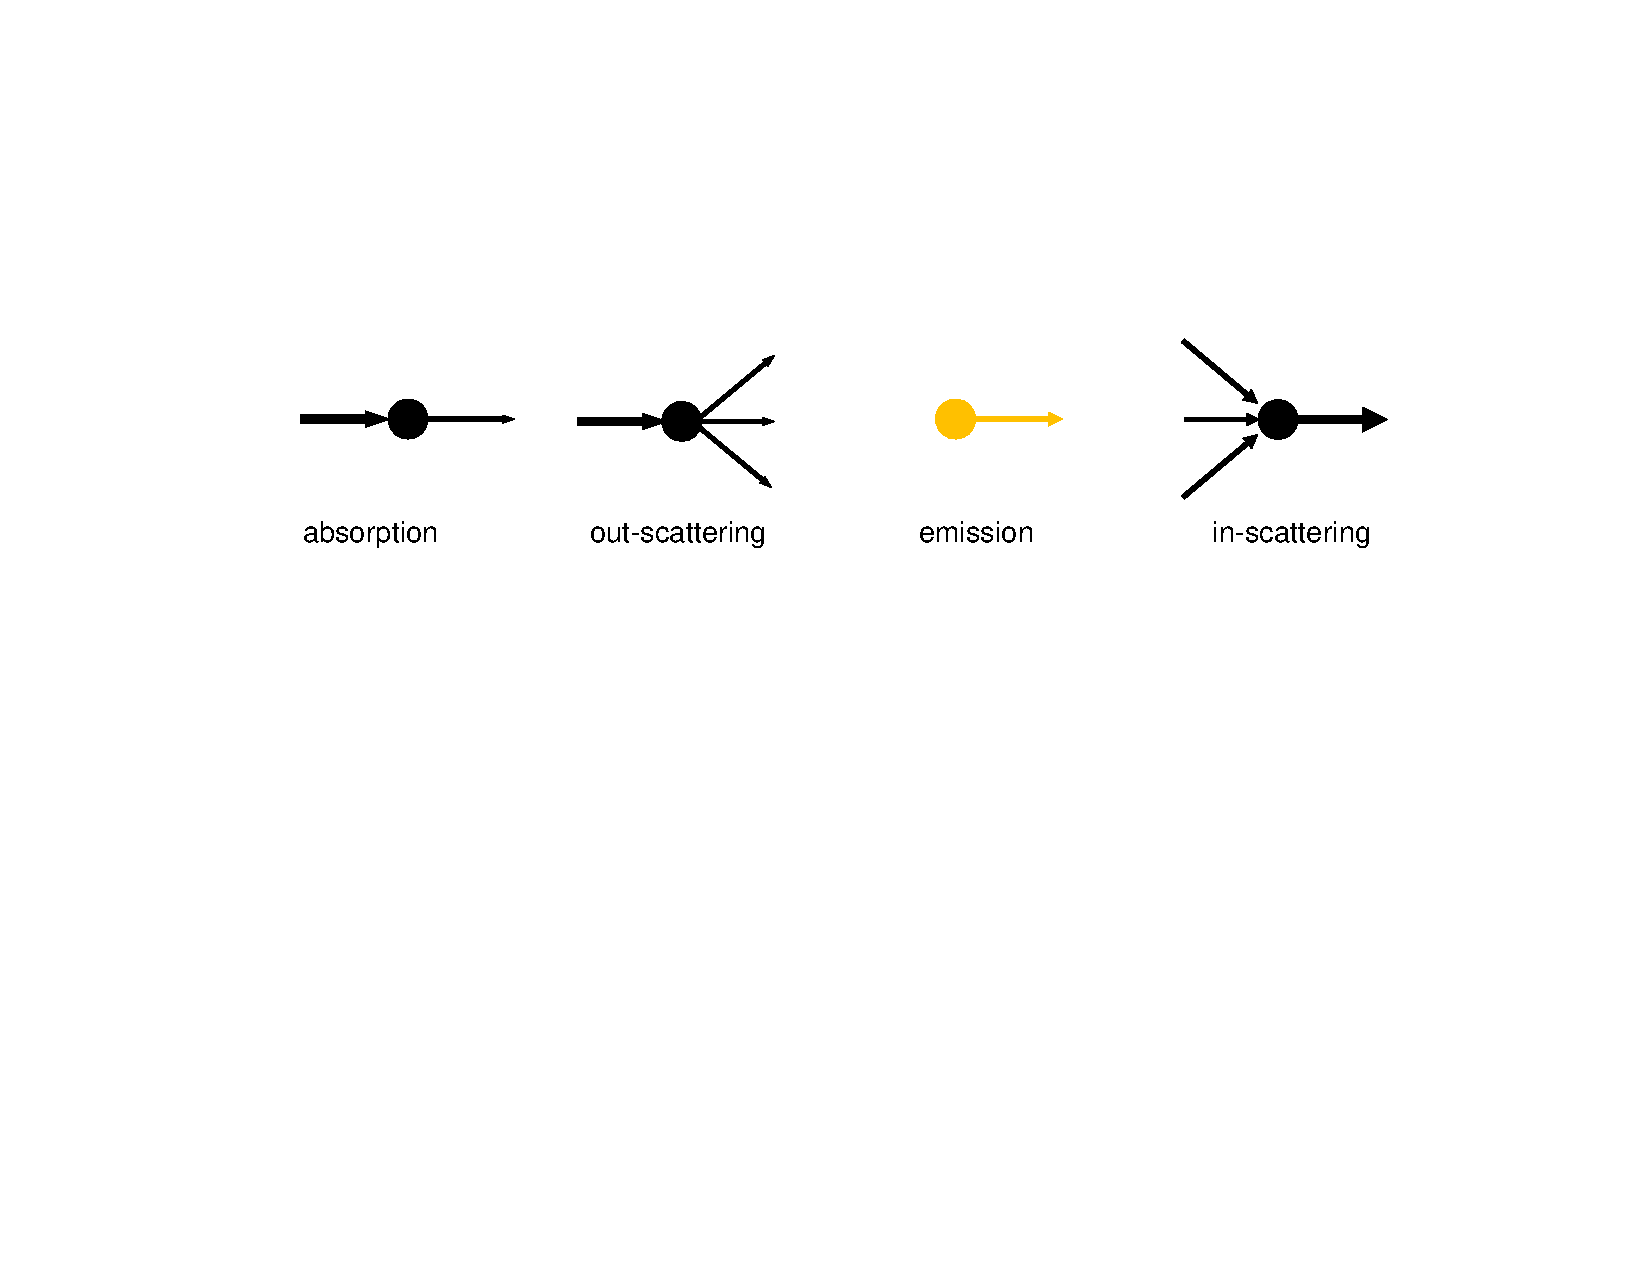
\includegraphics[width=6.0in]{FIGURES/rte_setup}
\end{center}
\caption[Diagram illustrating components of the radiation
transport equation]{Diagram illustrating components of the
radiation transport equation.  Absorption and out-scattering terms
decrease radiance.  Emission and in-scattering terms increase
radiance.} \label{figRadiance}
\end{figure}

% ----  Approximating the Radiation Transport Equation ------------------------

\subsection{Approximating the Radiation Transport Equation}

The RTE may be simplified in several ways depending on which terms
are included or ignored.  This section derives an approximate
solution in which the in-scattering integral term in
(\ref{eq:fullrte}) is neglected and the absorption and
out-scattering coefficients are combined (both are loss terms)
using $\sigt=\siga+\sigs$.  This simplification then only includes
interactions between light and smoke due to absorption,
out-scattering and emission.  Note that the Beer-Lambert law
results if the emission term is also dropped.

Equation (\ref{eq:fullrte}) is then approximated by neglecting the
integral term and using $\sigt=\siga+\sigs$ to obtain

\begin{eqnarray}
\dLdx&=&-\sigt C(x) + \siga C_e(x)\\
 C(x_0)&=&C_0
\end{eqnarray}

This equation may be solved by rearranging terms and applying the
integrating factor $\exp(\int_{x_0}^x \sigts \dx{s})$ obtaining

\begin{eqnarray}
\intf{x_0}{x}\left(\dLdx+\sigt C(x)\right)&=&  \intf{x_0}{x}\siga \Le\\
\ddx\left(\intf{x_0}{x} C(x)\right)&=& \intf{x_0}{x}\siga \Le
\end{eqnarray}

Integrating both sides and substituting the integration limits
results in

\begin{eqnarray}
\left.\intf{x_0}{x} C(x)\right|_{x_0}^{x_N}&=& \int_{x_0}^{x_N}\intf{x_0}{x}\siga \Le \dx{x} \\
\intf{x_0}{x_N} C(x_N)-C_0&=& \int_{x_0}^{x_N}\intf{x_0}{x}\siga \Le \dx{x}
\end{eqnarray}

Solving for $C(x_N)$ after noting that
$\intff{x_0}{x}-\intff{x_0}{x_N}=-\intff{x}{x_N}$ results in

\begin{eqnarray}
C(x_N)&=&\intmf{x_0}{x_N} C_0+ \int_{x_0}^{x_N}\intmf{x}{x_N}\siga
\Le \dx{x}
\end{eqnarray}

\noindent which may be simplified to

\begin{equation}
\label{eq:rtesoln}
 C(x_N)=\tau(x_0,x_N)C_0 + \int_{x_0}^{x_N}\tau(x,x_N)\siga\Le \dx{x}
\end{equation}

\noindent after defining $\tau(a,b)$ as
\begin{equation}
\label{eq:optdepth}
\tau(a,b)=\intmf{a}{b}
\end{equation}
which represents the optical depth between $a$ and $b$.  As noted earlier, if the emission term is neglected and $\sigma_t(x)=\sigma_t$ is constant over a path with length
$L=x_N-x_0$, then (\ref{eq:rtesoln}) simplifies to
\begin{eqnarray}
 \frac{C(x_N)}{C_0}=\exp(-\sigma_tL)
\end{eqnarray}
which is the Beer-Lambert law.

% -------------------  Discretizing the Radiation Transport Equation ------------------------

\subsection{Discretizing the Radiation Transport Equation}
\newcommand{\htau}[1]{\tau_{#1}^{N-1}}
\newcommand{\halpha}[1]{\alpha_{#1}^{N-1}}
\newcommand{\sigai}[1]{\sigma_{a,#1}}
\newcommand{\Lei}[1]{C_{e,#1}}
\newcommand{\Lhatj}[1]{C_{#1}^N}
\newcommand{\Lhatjj}[1]{\hat{C}_{#1}^N}
\newcommand{\Chatjj}[1]{\hat{C}_{#1}^N}
\newcommand{\Leii}[1]{\hat{C}_{e,#1}}

The approximate RTE solution given in (\ref{eq:rtesoln}) is
discretized by converting integral terms into Riemann sums. Figure
\ref{fig:smokediscretesetup}\ illustrates the terms used to
perform these discretizations.  The path is split into $N$ parts
each with length $\Delta x=(x_N-x_0)/N$.  The coordinate system is
set up so that the initial radiance, $C_0$, is located at $x_0$,
most distant from the observer and the final radiance, $C_N$, is
located at $x_N$ closest to the observer.

\begin{figure}[\figoptions]
\begin{center}
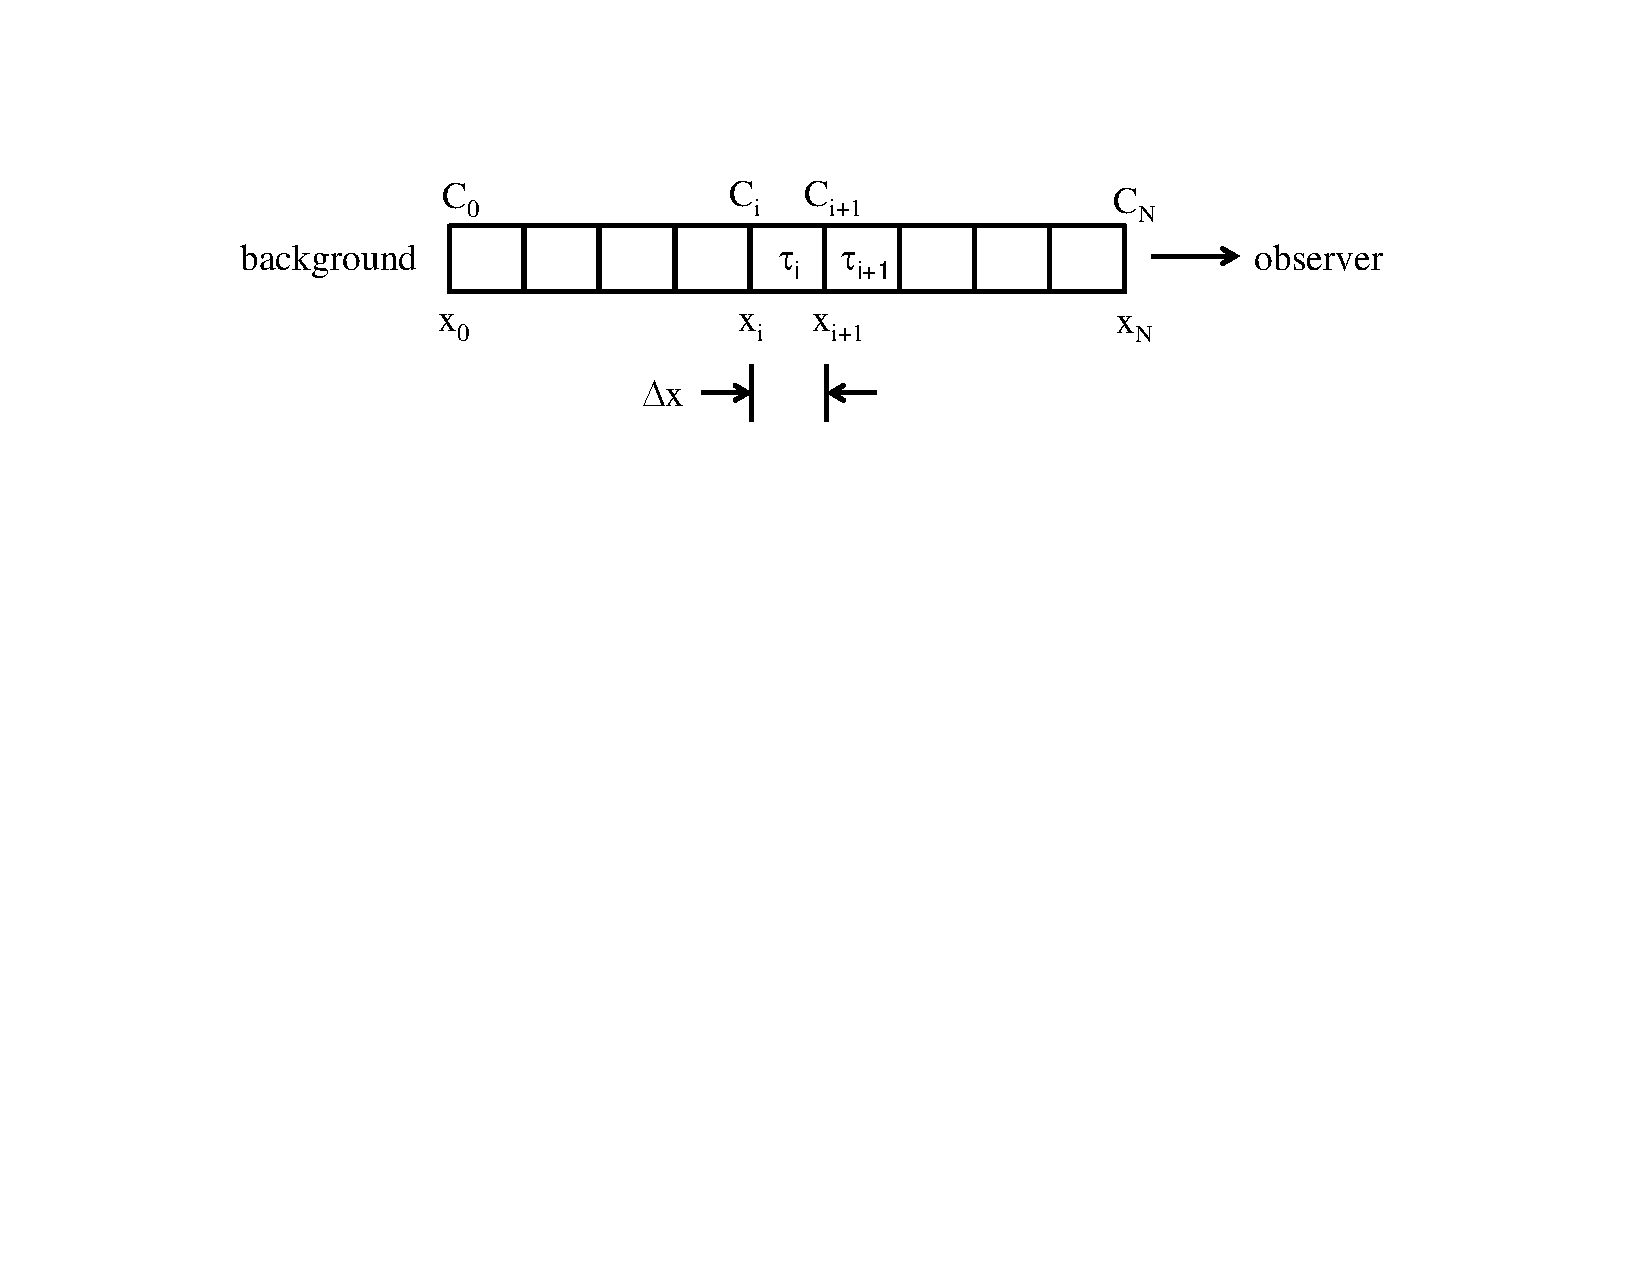
\includegraphics[width=5.0in]{FIGURES/smoke_discrete_setup}
\end{center}
\caption[Setup for discretizing the equations used to model
radiance within a column of 3D smoke data.]{Setup for discretizing
the equations used to model radiance within a column of 3D smoke
data. The transparency across the interval from $x_i$ to $x_{i+1}$
is $\tau_i$. The transparency across the intervals from $x_i$ to
the observer is the product of individual transparencies or
$\tau_i\tau_{i+1}\cdots\tau_{N-1}$} \label{fig:smokediscretesetup}
\end{figure}

The optical depth, $\tau(a,b)$, defined in (\ref{eq:optdepth}) is
discretized using a Riemann sum  after defining sample points
$s_j=x_0+j\Delta s$ for $j=0$ to $N$ with spacing $\Delta
s=(x_N-x_0)/N$ to obtain

\begin{eqnarray}
\htau{i}=\tau(x_i,x_N)&=&\exp\left(-\int_{x_i}^{x_N}\sigma_t(s)\dx{s}\right)\approx\exp\left(-\sum_{j=i}^{N-1}\sigma_t(s_j)\Delta s\right)\\
&=&\prod_{j=i}^{N-1}\exp\left(-\sigma_t(s_j)\Delta s\right)=\prod_{j=i}^{N-1}\tau_j
\end{eqnarray}

\noindent where $\tau_j=\exp\left(-\sigma_t(s_j)\Delta s\right)$
represents the transparency over one discretization interval.
For~$i=N-1$~to~$0$, the optical depth $\htau{i}$ may be computed
recursively using
\begin{eqnarray}
\label{eq:tauhat_recurse}
\htau{i}&=&\htau{i+1}\tau_i
\end{eqnarray}
\noindent where the recursion is initiated with $\htau{N}=1$.
Substituting $1-\halpha{i}=\htau{i}$ and $1-\alpha_i=\tau_i$ into
(\ref{eq:tauhat_recurse}) gives
\begin{eqnarray}
1-\halpha{i}=(1-\halpha{i+1})(1-\alpha_i)=1-\halpha{i+1} - \alpha_i + \halpha{i+1}\alpha_i
\end{eqnarray}
which simplifies to
\begin{eqnarray}
\label{eq:alpha2}
\halpha{i}&=&\halpha{i+1} + (1-\halpha{i+1})\alpha_i
\end{eqnarray}

Similarly, the radiance given by the RTE solution $C(x_N)$ in
(\ref{eq:rtesoln}) may be discretized to obtain

\begin{eqnarray}
C_{N} = \htau{0}\,C_0 +
\sum_{i=0}^{N-1}\htau{i}\,\sigai{i}\,\Lei{i}\,\Delta x
\end{eqnarray}

\noindent where $\sigma_{a,i}=\sigma_a(x_i)$, $\Lei{i}=C_e(x_i)$,
$x_i=x_0+i\Delta x$ and $\Delta x=(x_N-x_0)/N$. This simplifies to

\begin{equation}
\label{eq:discrete_rte2}
C_N = \htau{0}C_0 + \sum_{i=0}^{N-1}\htau{i}\,\Leii{i}
\end{equation}

\noindent where $\Leii{i}=\sigma_{a,i}C_{e,i}\Delta x$.  If
$\Leii{i}$ is interpreted as the emitted color of the fire or
heated gas at location $i$ and $C_0$ is interpreted as the color
of the light source {\em behind}\ the smoke, then
(\ref{eq:discrete_rte2}) restated in words gives color seen by the
observer computed as a weighted average of source and emitted
colors where each weight is the optical depth from the observer to
the corresponding color location.  These emitted colors can be
determined from a blackbody temperature curve or from a colormap
meant to show variations in temperature in terms of color.


The terms in (\ref{eq:discrete_rte2}) are summed from back to
front meaning that the location of the $i=0$ term is farthest from
the observer, while the location of the $i=N-1$ term is closest.
We wish to perform this sum in reverse order, from front to back
so that the sum may be terminated early if additional
contributions would not significantly change the result.

Therefore, to compute $C_N$, let $\Chatjj{j}$ denote the partial
sum using terms $i=j$ through $i=N-1$ in the summation term in
(\ref{eq:discrete_rte2}).  Using this notation
$\hat{C}_N=\htau{0}C_0+\Chatjj{0}$ . Then

\begin{eqnarray}
\label{eq:recurse1}
\Chatjj{j} &= &\sum_{i=j}^{N-1}\htau{i}\,\Leii{i}\\
\label{eq:recurse2}
\Chatjj{j+1}     &= &\sum_{i=j+1}^{N-1}  \htau{i}\,\Leii{i}
\end{eqnarray}

Subtracting (\ref{eq:recurse2}) from (\ref{eq:recurse1}) and solving
for $\Chatjj{j}$ results in
\begin{eqnarray}
\label{eq:color}
\Chatjj{j}&=&\Chatjj{j+1}+\htau{j}\,\Leii{j}
\end{eqnarray}
The strategy then for volume rendering an image is for each pixel
in the 2D projected image to
\begin{enumerate}
\item convert the background radiance $C_0$ to a color,

\item convert the emitted radiances along the integration path to
colors and

\item form a weighted average of these colors using either
equation (\ref{eq:discrete_rte2}) or (\ref{eq:color}) where the
weights are optical depths obtained using (\ref{eq:alpha2}) .

\end{enumerate}
The conversion from radiance to color may be based on a blackbody
temperature curve if realistic flame colors are the goal or
arbitrary if only a qualitative view of the fire is the goal.
Equations (\ref{eq:alpha2}) and ({\ref{eq:color}) are equivalent
to the recursions presented in Ref.~\cite[Chapter 39]{gpugems} for
performing volume rendering.

% -------------------  Splitting the Radiation Transport Equation ------------------------

\subsection{Splitting the Radiation Transport Equation}
This section discusses splitting the Radiation Transport
Equation (RTE), so that it may be solved separately on multiple
meshes or multiple slice planes.  The final solution is then
obtained by  appropriately combining solutions obtained on each
mesh or slice plane.

It is more practical to draw smoke one mesh at a time when
visualizing multiple mesh cases since required data may not be
easily accessible from all meshes, especially if the
GPU\footnote{graphics processing unit of the video card}\ is used
for drawing.  The RTE solution or equivalently the computed
radiance and smoke opacity require  properties for the entire line
of sight which may encompass more than one data mesh.  This
section discusses how  radiance and opacity may be computed by
combining solutions from each individual mesh along the line of
sight.  For example, as illustrated in Fig. \ref{figsmokesetup3},
consider an interval $[x_0,x_N]$ that is split at $D$ into two
sub-intervals $[x_0,D]$ and $[D,x_N]$.  The goal then is to
compute a radiance and opacity for $[x_0,x_N]$ using radiances and
opacities computed on  the two sub-intervals.

\begin{figure}[\figoptions]
\begin{center}
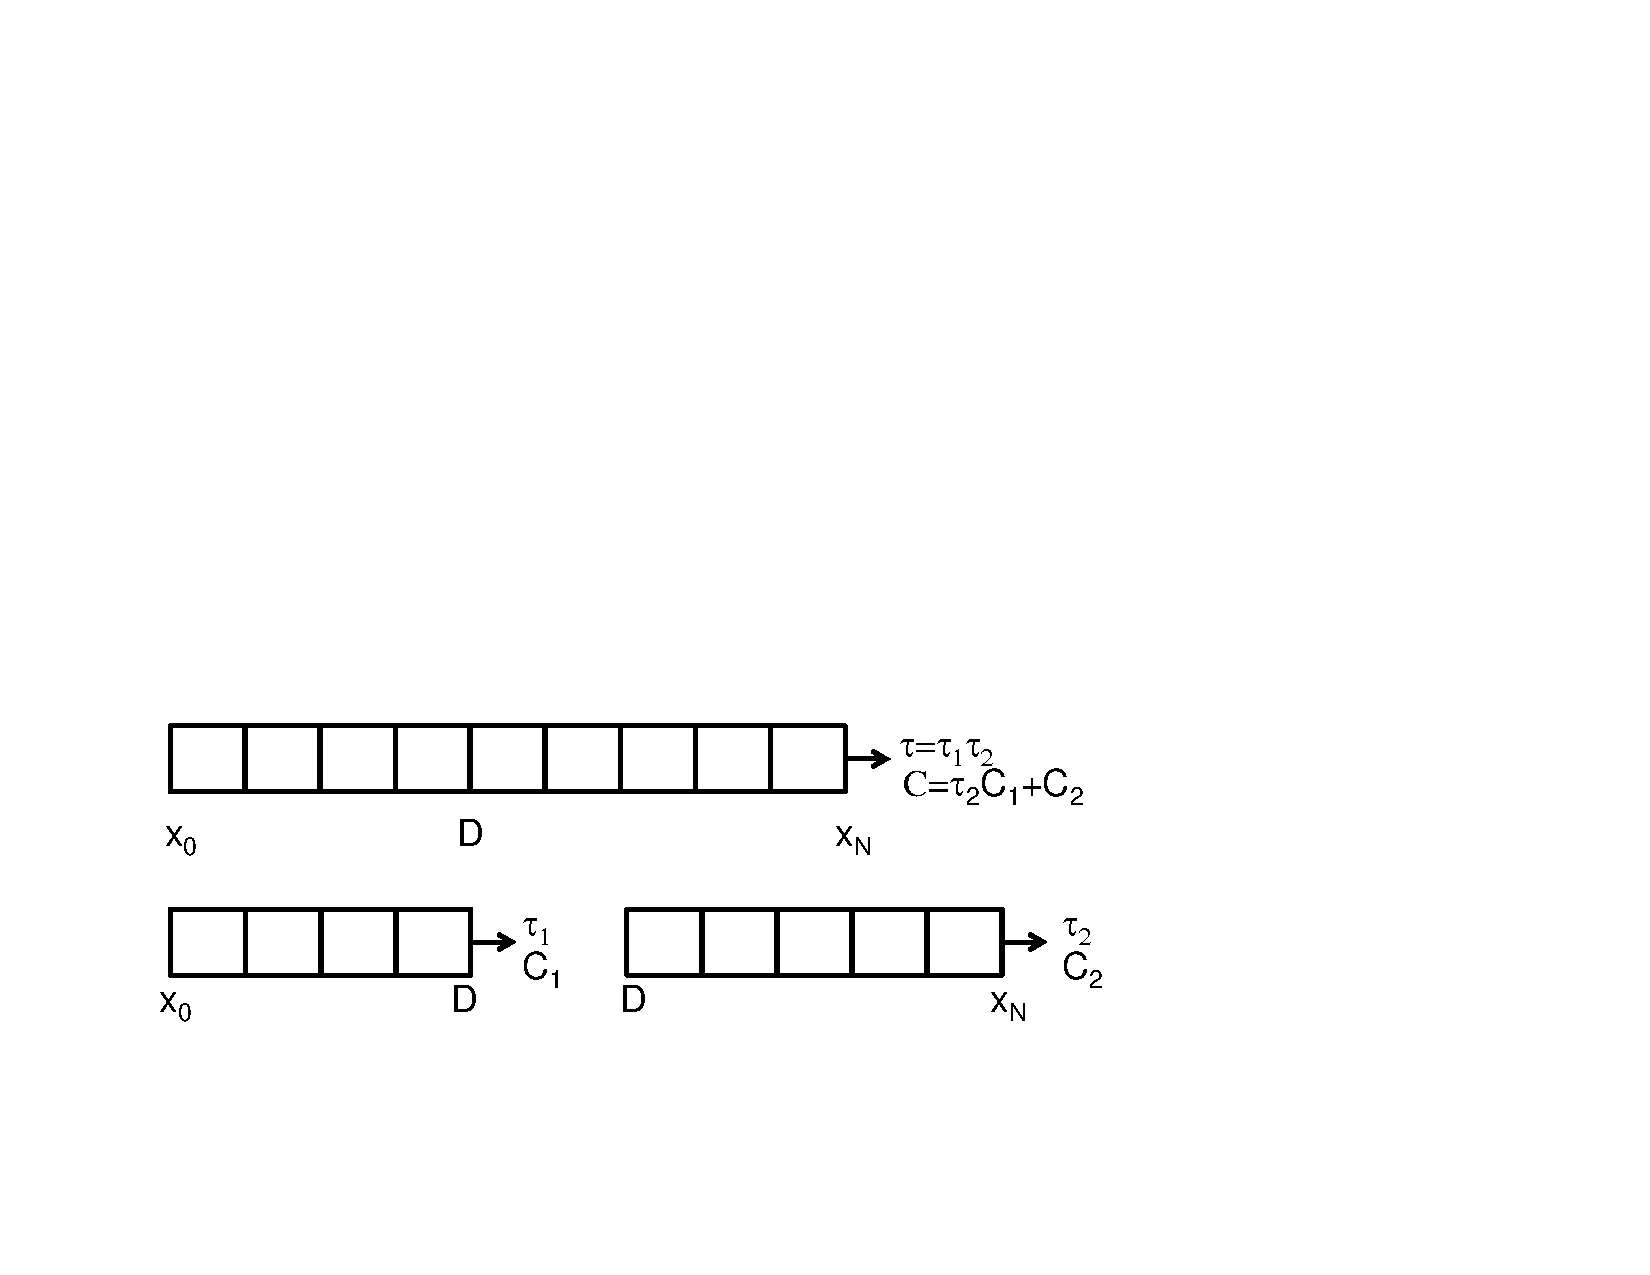
\includegraphics[width=4.0in]{FIGURES/smoke_setup3}
\end{center}
\caption {Solutions to the RTE on two sub-intervals are combined
to form a solution to the RTE for the merger of these intervals.}
\label{figsmokesetup3}
\end{figure}

Let $C$ be a radiance computed on $[x_0,x_N]$ and $C_1$ and $C_2$
be radiances computed on two sub-intervals of $[x_0,x_N]$.
Likewise, let $\tau$ be an optical depth computed on $[x_0,x_N]$
and $\tau_1$ and $\tau_2$ be optical depths computed on two
sub-intervals of $[x_0,x_N]$. From (\ref{eq:rtesoln}) and
(\ref{eq:optdepth}), the radiance $C$ and optical depth $\tau$ are
given by

\begin{eqnarray}
C&=&\int_{x_0}^{x_N}\tau(x,x_N)\sigma_a(x)C_e(x)\dx{x}\\
\tau&=&\tau(x_0,x_N)
\end{eqnarray}

Likewise, the radiances $C_1$ and $C_2$ and optical depths
$\tau_1$ and $\tau_2$ for the intervals $[x_0,D]$ and $[D,x_N]$
are given by

\begin{eqnarray}
C_1&=&\int_{x_0}^{D}\tau(x,D)\sigma_a(x)C_e(x)\dx{x}\\
C_2&=&\int_{D}^{x_N}\tau(x,x_N)\sigma_a(x)C_e(x)\dx{x}\\
\tau_1&=&\tau(x_0,D)\\
\tau_2&=&\tau(D,x_N)
\end{eqnarray}

The optical depth $\tau$ can be split into two parts giving
\begin{eqnarray}
\tau&=&\tau(x_0,x_N)=\tau(x_0,D)\tau(D,x_N)=\tau_1\tau_2
\end{eqnarray}
since from (\ref{eq:optdepth}) it can be shown that for any $x$, $\tau(a,b)=\tau(a,x)\tau(x,b)$.
The radiance $C$ can also be split into two parts giving
\begin{eqnarray}
C&=&\int_{x_0}^{x_N}\tau(x,x_N)\sigma_a(x)C_e(x)\dx{x}\\
&=&\int_{x_0}^{D}\tau(x,x_N)\sigma_a(x)C_e(x)dx+\int_{D}^{x_N}\tau(x,x_N)\sigma_a(x)C_e(x)\dx{x}\\
&=&\tau(D,x_N)\int_{x_0}^{D}\tau(x,D)\sigma_a(x)C_e(x)dx+\int_{D}^{x_N}\tau(x,x_N)\sigma_a(x)C_e(x)\dx{x}\\
&=&\tau_2C_1+C_2
\end{eqnarray}

Summarizing, full-interval values $C$ and $\alpha$ may be written
in terms of sub-interval values $C_1$, $C_2$, $\alpha_1$ and
$\alpha_2$ using

\begin{eqnarray}
\label{eq:alpha_summary}
\tau&=&\tau_1\tau_2\\
\label{eq:C_summary}
C&=&\tau_2C_1+C_2
\end{eqnarray}

Equations (\ref{eq:alpha_summary}) and (\ref{eq:C_summary}) may
then be used to draw smoke and fire one mesh at a time.  These two
equations are also the basis for combining RTE solutions obtained
on multiple slice planes, which is discussed next.

% -------------------  A Solution using Slices ------------------------

\section{Slice Rendering}
A slice rendering algorithm for visualizing smoke consists of
splitting the RTE across individual slice planes within a single
mesh.  The 3D computational domain is partitioned into a series of
2D slices.  The RTE is then solved on each slice.  Each slice
solution only accounts for conditions between adjacent slices.
The individual partially transparent slice solutions are then
combined using video hardware to form the final image.   Problems
can occur with numerical round off error if two slices are too
close together which require solution methods  involving data
volumes rather than data slices. These methods are discussed in
the next section.

There are many ways to slice a 3D data set.  The slice orientation
is chosen to be the one most perpendicular to the viewer's line of
sight, for which possible choices are slice planes parallel to the
three cartesian coordinate planes (XY, XZ, YZ) or planes diagonal
to the data.  The opacity at each grid node is computed using the
distance $\Delta x$ between adjacent YZ planes and soot density
data computed by the fire model.  If slice orientations other than
YZ are displayed, then opacities are adjusted if the distance
between planes is different than $\Delta x$.  Opacity data is
computed and compressed using run length encoding as a
preprocessing step and decompressed one frame at a time as data is
displayed.

% -------------------  Computing Color ------------------------

\subsection{Computing Color}

Smokeview visualizes smoke and fire by drawing a series of triangles in equally spaced parallel planes.  
Color for these triangles are assigned using temperature or hrrpuv (heat release per unit volume) values.
Transparency is assigned using soot density, the greater the soot density, the more opaque the triangle.

An example color map is illustrated in Fig.
\ref{fig:colormaps}.  This maps is split into two parts.  The left half is used
to color non-burning regions, the right half is used to color burning regions.
An hrrpuv cutoff value denoted ${\rm hrrpuv}_{\rm cutoff}$ is used to
determine which half of the color map is used to color a given region.
If an hrrpuv value is below the cutoff
then smoke is drawn using the left have of the color map, otherwise if an hrrpuv value is above the cutoff
then fire colors are drawn using the right half of the color map.  The color map is defined as a table
of 256 red, green, blue color triplets.  A formula giving a color index for a given hrrpuv value is given by

\newcommand{\hrr}{{\rm hrr}}
\newcommand{\hrrcutoff}{{\rm hrr}_{\rm cutoff}}
\newcommand{\hrrmax}{{\rm hrr}_{\rm max}}

\begin{eqnarray}
\mbox{color index}=\left\{
\begin{array}{ll}
  127\frac{\hrr}{\hrrcutoff} & 0 \le \hrr \le \hrrcutoff \\
  127 + 128\frac{\hrr-\hrrcutoff}{\hrrmax-\hrrcutoff} & \hrrcutoff \le \hrr \le \hrrmax
\end{array}
\right.
\end{eqnarray}

\begin{figure}[\figoptions]
\begin{center}

\includegraphics[width=5.0in]{FIGURES/colorbar_fire2}
\end{center}
\caption[Example colormap used for converting temperature or hrrpuv values to color.]
{Example colormap used for converting temperature or hrrpuv values to color.}
\label{fig:colormaps}
\end{figure}

% -------------------  Computing Opacity ------------------------

\subsection{Computing Opacity}
Computing opacity at slice plane nodes is illustrated in Fig.
\ref{figsmokesetup}. A ray travels from the background to the
observer through intervening smoke. Light is absorbed or scattered
by the smoke as the ray passes each slice plane. Emission effects
are accounted for by coloring the smoke.  Scattering effects
presently are only accounted for in the value of the total mass
extinction coefficient.  Light losses are assumed to be from both
absorption and scattering. The obscuration is computed along each
ray one grid plane at a time, using the Beer-Lambert law as
follows.  The $\alpha=1-\tau$ values are pre-computed by FDS using
the Beer-Lambert law~\cite{Siegel:2001}

\begin{equation}
\label{eq:alpha}
\alpha=1-\exp(-\sigma_t\Delta x)
\end{equation}

\noindent for a particular view direction (down the $x$~axis)
where $\Delta x$ is this distance between two grid planes and as
before $\sigma_t=\sigma_a+\sigma_s$ is the total mass extinction
coefficient.  The Beer-Lambert law is an empirical relationship
relating light absorption to the material properties of the medium
the light is travelling through, in this case soot or smoke.

\begin{figure}[\figoptions]
\begin{center}
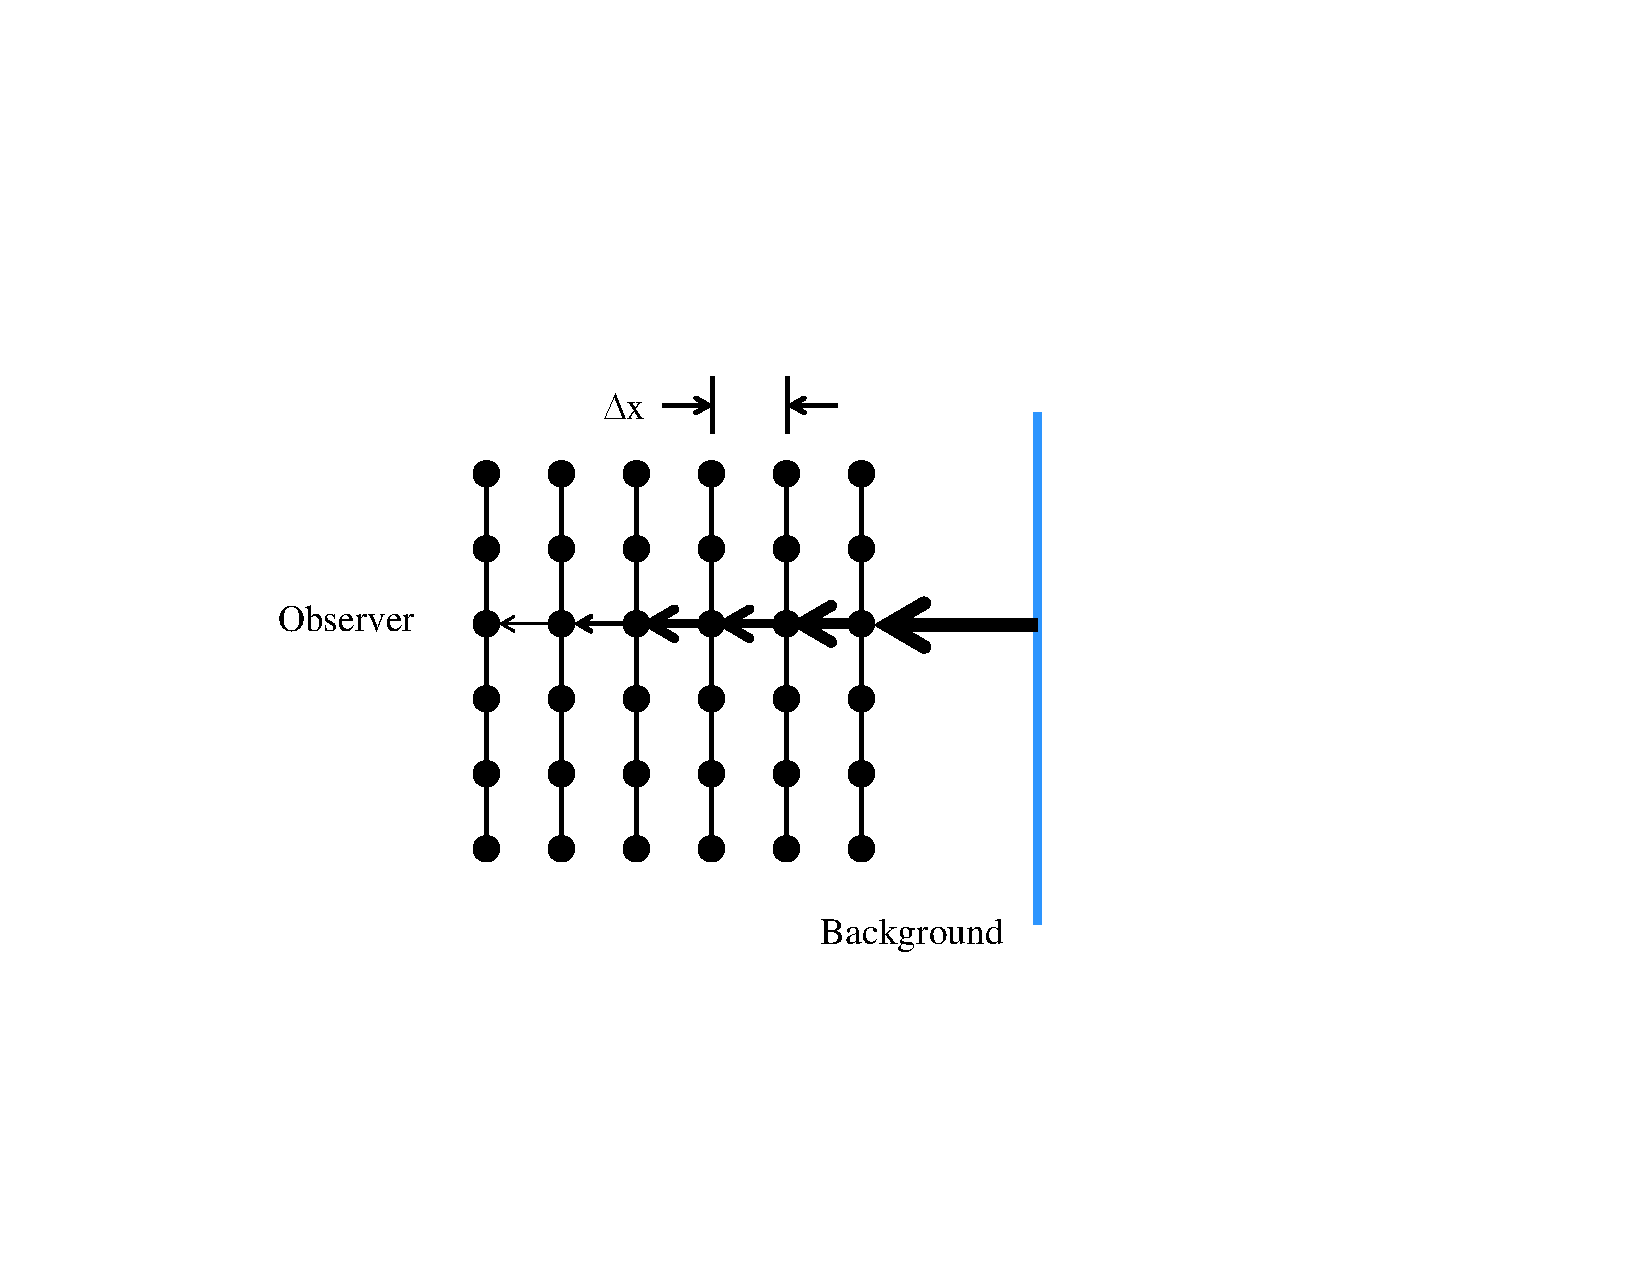
\includegraphics[width=4.0in]{FIGURES/smoke_setup}
\end{center}
\caption[Light emitted from the background is obscured by intervening smoke.]
{Light emitted from the background is obscured by intervening smoke.
}
\label{figsmokesetup}
\end{figure}

The $\alpha$ parameter in (\ref{eq:alpha}) is used by
OpenGL~\cite{OpenGLRed} to blend smoke planes with the current
background.  The $\alpha$ parameter used here also represents an
opacity, 0.0, for completely transparent, and 1.0 for completely
opaque.

% -------------------  Adjusting Opacity ------------------------

\subsection{Adjusting Opacity}

The absorption parameter, $\alpha$, needs to be adjusted for view
directions not aligned with the axis orthogonal to the viewing
planes (see Fig. \ref{figray}).  The absorption coefficient also
needs to be adjusted when the distance between adjacent smoke
planes changes, or viewing planes are skipped.

\begin{figure}[\figoptions]
\centerline{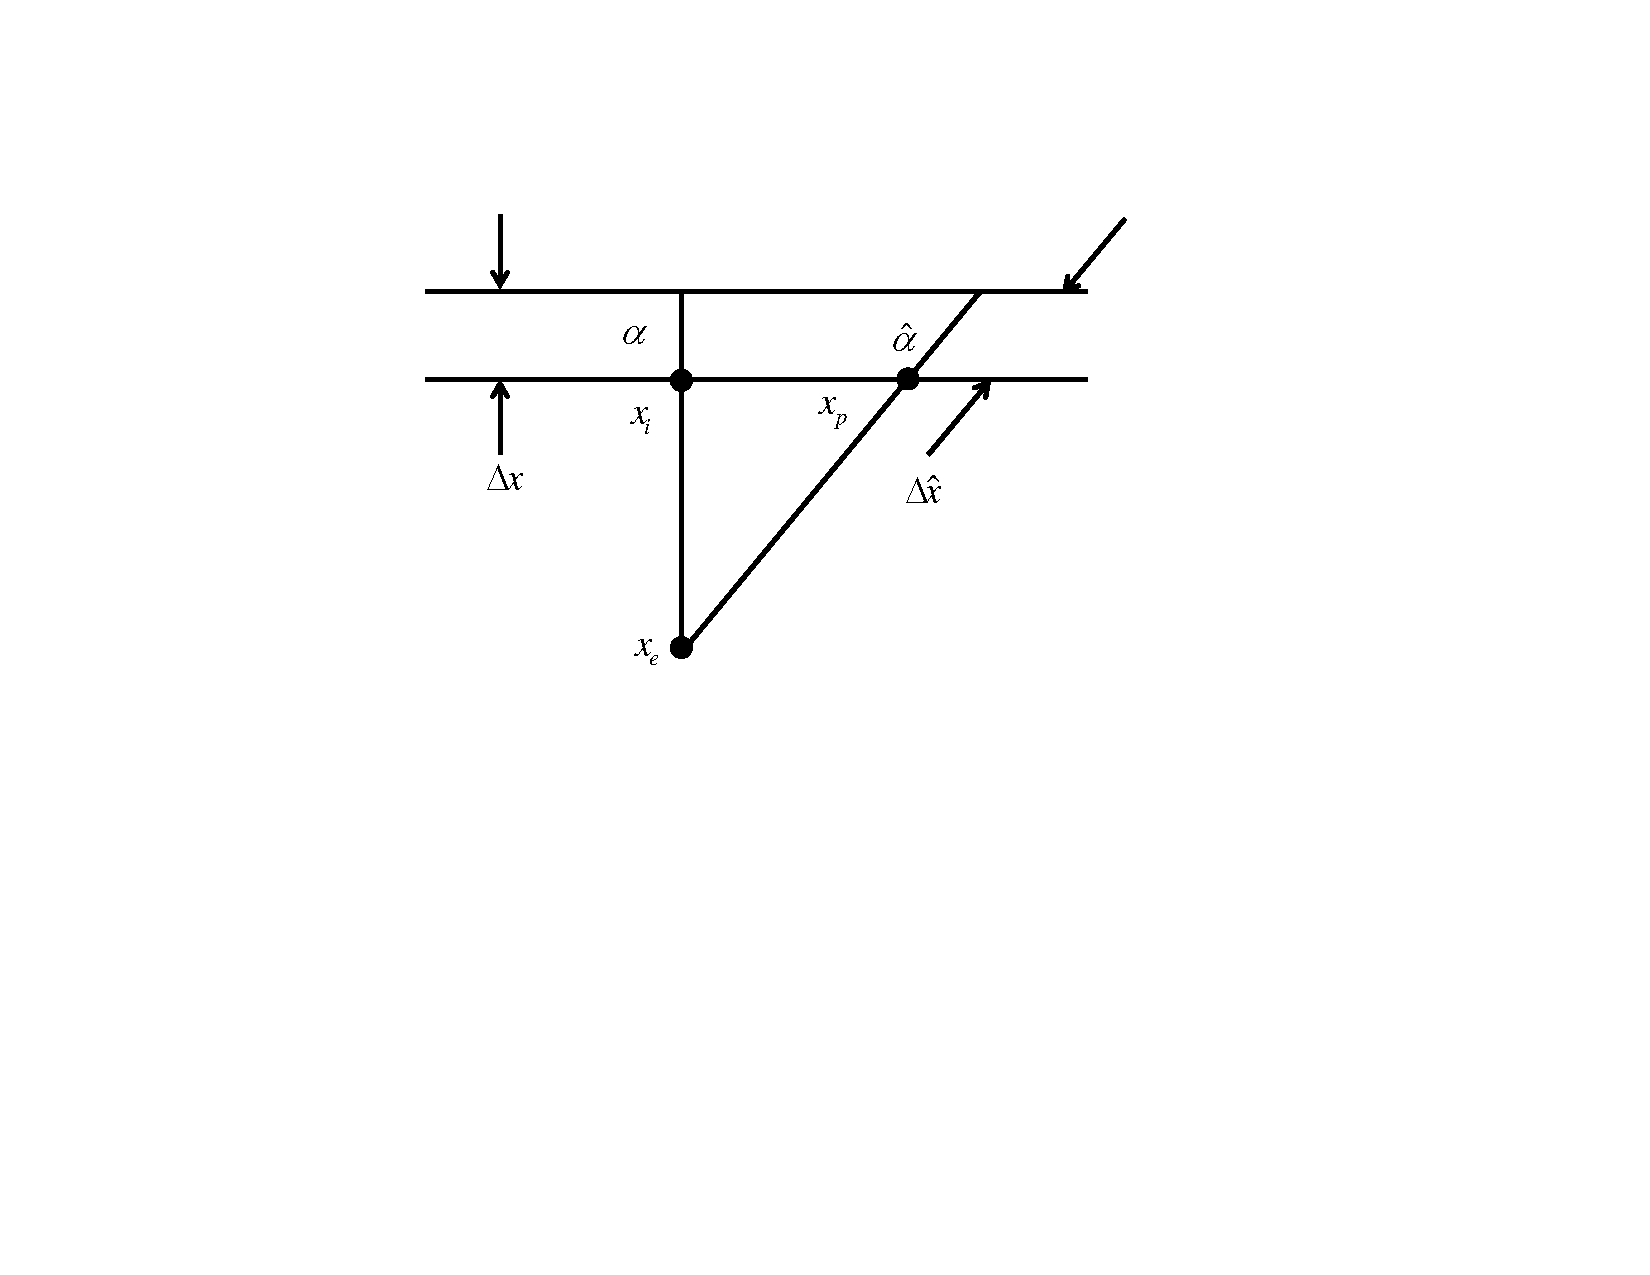
\includegraphics[width=3.5in]{FIGURES/forney_figure4}}
\caption [Diagram illustrating the adjustment required to the
opaqueness parameter, $\alpha$, for non-axis aligned views.] {
Diagram illustrating the adjustment required to the opaqueness
parameter, $\alpha$, for non axis aligned views. The adjusted
opacity $\hat{\alpha}$ along the $\Delta\hat{x}$ segment is
related to $\alpha$ value along the $\Delta x$ segment using
$(1-\hat{\alpha})=(1-\alpha)^{\Delta \hat{x}/\Delta x}$}
\label{figray}
\end{figure}

Ten million exponential operations per second are required to
display smoke with corrected $\alpha$'s at 10 frames per second if
the simulation has grid dimensions of $100\times 100\times 100$.
Recent advances in CPU and video hardware makes these types of
visualizations possible. These corrections may also be performed
in the video card (GPU), resulting in increased display rates
because the GPU performs the corrections simultaneously at all or
many of the grid nodes rather than one at a time as the CPU would.

The $\alpha$ obscurations are pre-computed using the distance
$\Delta x$ between adjacent planes along the $x$~axis. The
adjusted $\hat{\alpha}$ expressed in terms of $\Delta\hat{x}$ is
given by

\begin{equation}
\label{eq:adjusted}
\hat{\alpha}=1-\exp(-\sigma_t\Delta \hat{x})\\
\end{equation}

where $\Delta\hat{x}$ is the distance between planes along the
line of site.  Equations (\ref{eq:alpha}) and (\ref{eq:adjusted})
may be used to solve for $\hat{\alpha}$ in terms of $\alpha$ to
obtain

\begin{equation}
\label{eq:alphahat}
\hat{\alpha}=1-(1-\alpha)^{\Delta\hat{x}/\Delta x}
\end{equation}

after noting that

\begin{eqnarray}
1-\hat{\alpha}=\exp(-\sigma_t\Delta\hat{x})=\exp(-\sigma_t\Delta
x)^{\Delta\hat{x}/\Delta x}=(1-\alpha)^{\Delta\hat{x}/\Delta x}
\end{eqnarray}

The computation of (\ref{eq:alphahat}) is expensive because the
exponential is computed at each grid node for every time step.  In
addition, numerical cancellation may occur for small $\alpha$
leading to loss of significant digits. Both problems may be solved
by expanding (\ref{eq:alphahat}) in a Taylor series and keeping
only the first few terms:

\begin{eqnarray}
\hat{\alpha}\approx \alpha r -
\frac{\alpha^2}{2}r(r-1)+\frac{\alpha^3}{6}r(r-1)(r-2)
\end{eqnarray}

where $r=\sec(\theta)=\Delta \hat{x}/\Delta
x=||x_p-x_e||/n\cdot(x_p-x_e)$, $n$ is the unit vector normal to
the current plane being drawn, $\theta$ is the angle between the
view direction and $n$, $x_e$ is the observers position and $x_p$
is the vertex being drawn (along the view direction).  These terms
are illustrated in Fig. \ref{figray}.

When planes are skipped, (\ref{eq:alphahat}) may be simplified.
In particular, when every 2nd plane is skipped,
$\Delta\hat{x}/\Delta x=2$, so that (\ref{eq:alphahat}) simplifies
to

\begin{eqnarray}
\hat{\alpha}=1-(1-\alpha)^2=2\alpha-\alpha^2
\end{eqnarray}

The video hardware uses $\alpha$ values contained in the smoke
planes to obscure the background much like a camera uses a neutral
density filter to darken a scene.  Extending the analogy,
Smokeview uses one spatial/time varying {\em numerical}\ neutral
density filter for each plane of smoke data.  On a node by node
basis then, each smoke plane obscures the current image stored in
the OpenGL back buffer by the amount $(1-\alpha)$ to form a new
back buffer image.  Figure \ref{figplume} illustrates this process
showing several snapshots of a fire plume. The final image in the
lower right is the most realistic. A simplistic description of one
step of this process is given by

\begin{eqnarray}
\mbox{new buffer image} = (1-\alpha)\times \mbox{old buffer image}
\end{eqnarray}

\begin{figure}[\figoptions]
\begin{center}
\begin{tabular}{cc}

\includegraphics[height=4.0in]{FIGURES/splume_20_27}&
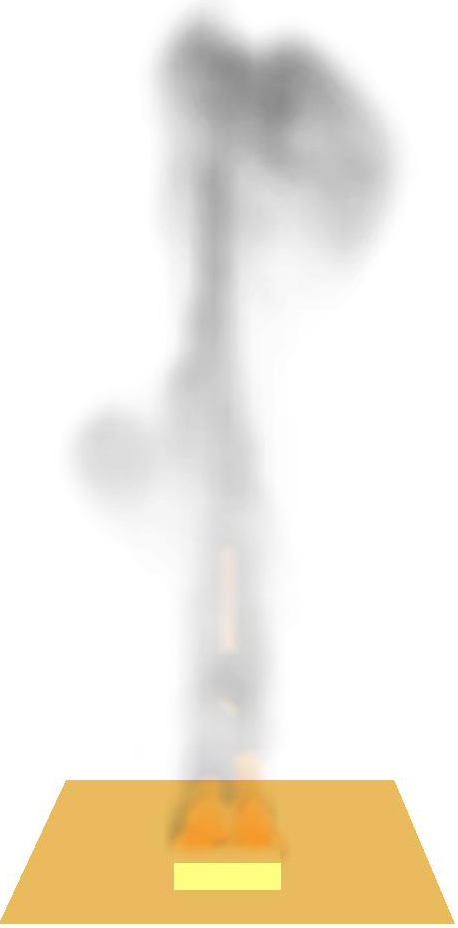
\includegraphics[height=4.0in]{FIGURES/splume_17_27}\\
8 slices&11 slices\\
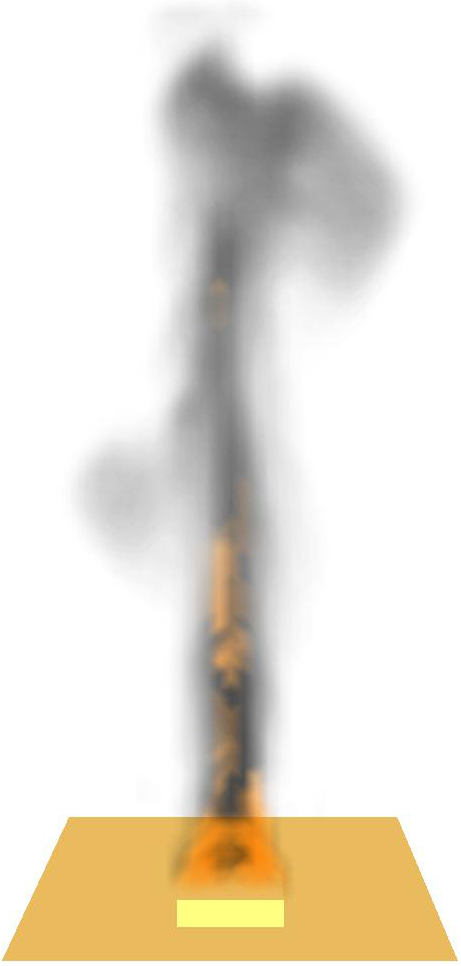
\includegraphics[height=4.0in]{FIGURES/splume_14_27}&
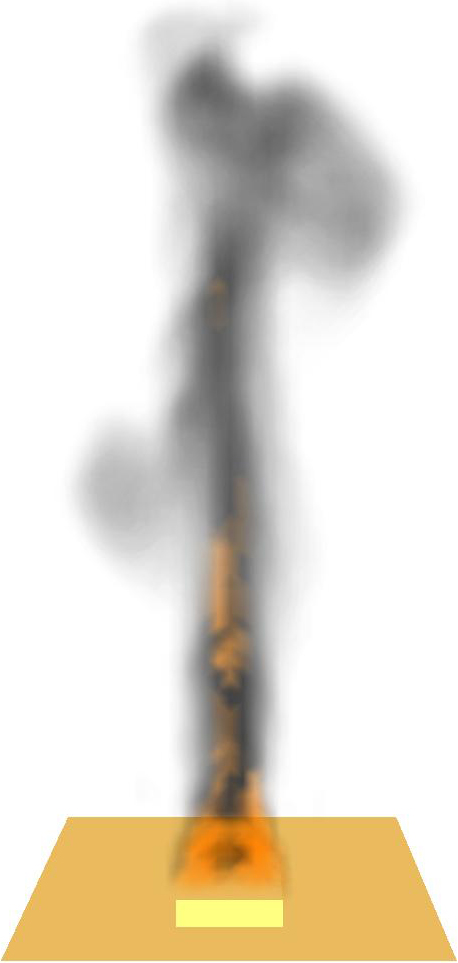
\includegraphics[height=4.0in]{FIGURES/splume_11_27}\\
14 slices&all slices
\end{tabular}
\end{center}
\caption [Smoke plume visualized using several vertical parallel
partially transparent planes.] {Smoke plume visualized using
several vertical parallel partially transparent planes. The smoke
plume looks more realistic as more slice planes are included to
form the image. } \label{figplume}
\end{figure}

\noindent This process is repeated for each smoke plane.

Figure \ref{figsmoke3d} illustrates this process showing smoke and
fire in a townhouse kitchen fire. The visualization is performed
by displaying a series of partially transparent planes. For
illustration, these planes are made more conspicuous (in Fig.
\ref{figsmoke3d}a) by skipping smoke planes (displaying every
third plane) and orienting them along the $x$~axis. Figure
\ref{figsmoke3d}b shows the visualization as it normally appears
with all slice planes shown and oriented along a plane most
perpendicular to the view direction.

\begin{figure}[\figoptions]
\begin{center}
\begin{tabular}{l}
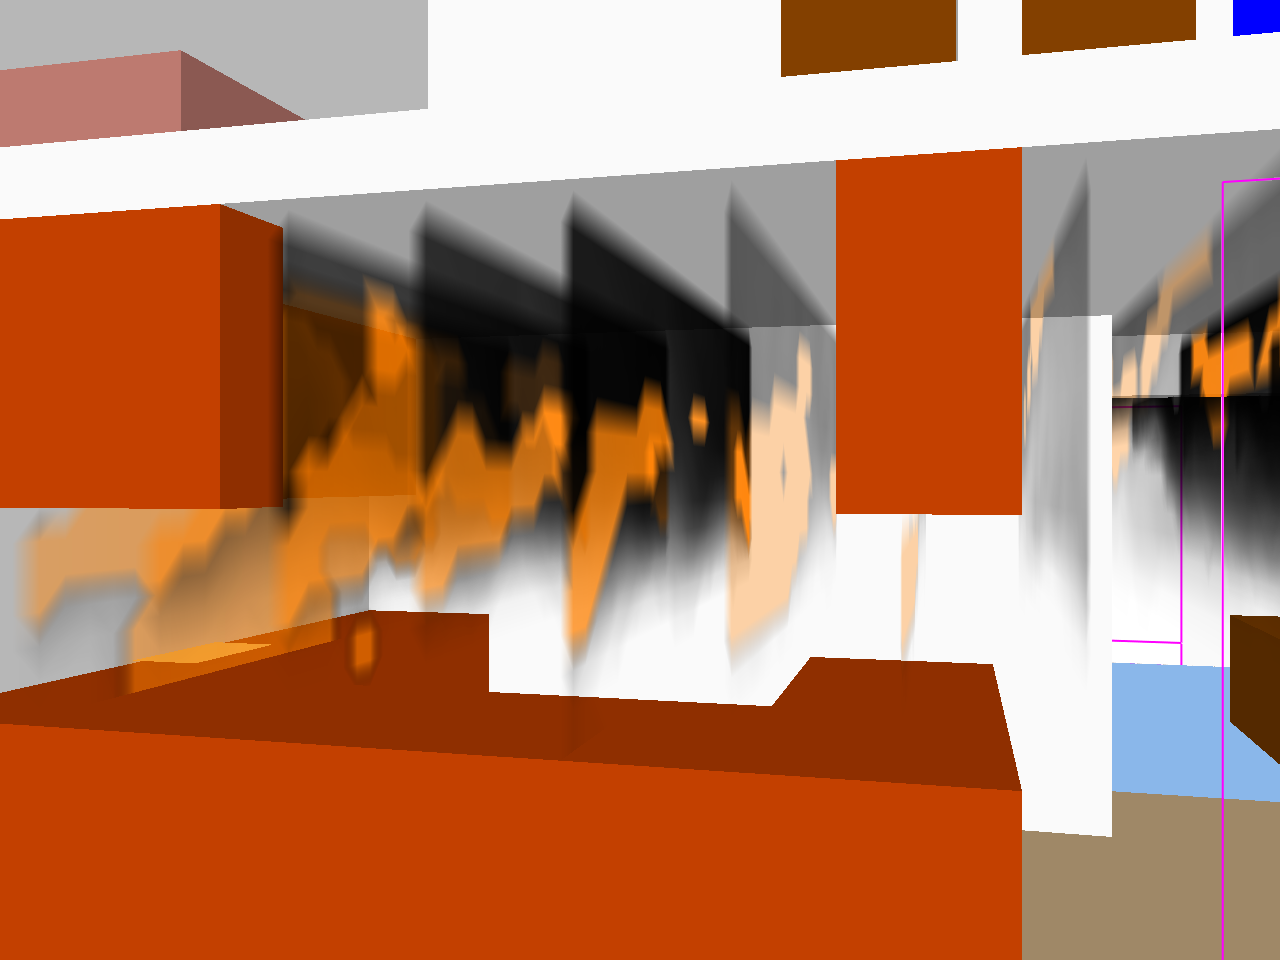
\includegraphics[height=3.75in]{FIGURES/thouse5c_skip}\\
a) slices skipped and oriented along `X' directions\\
\includegraphics[height=3.75in]{FIGURES/thouse5c_full}\\
b) all slices shown and oriented towards viewer \\
\end{tabular}
\end{center}
\caption[Realistic visualization of a townhouse kitchen fire
simulated using FDS.]{Realistic visualization of a townhouse
kitchen fire simulated using FDS. For illustrative purposes,
planes in the top image are oriented along the $x$~axis.  Planes
in the bottom image are aligned along the $y$~axis, the axis most
perpendicular to the line of sight.}
\label{figsmoke3d}%
\end{figure}

% -------------------  Orienting smoke planes ------------------------

\subsection{Orienting Slice Planes}

Smoke opacity data computed as described in the previous sections
is stored in a 3D array. This array corresponds to the solution
domain as set up in an FDS input file (or some other model). Smoke
planes are drawn in Smokeview through this data.  The orientation
is chosen to be most perpendicular to the viewer's line of sight.
A plane orientation exactly perpendicular to the view direction
could be drawn if one is willing to pay the added CPU cost of
interpolating opacity values between grid nodes.

Figure \ref{figDIRA} illustrates this process showing three view
directions and the corresponding smoke plane orientations that
would be used. Off-axis viewing is minimized by selecting the view
planes orientation that minimizes the angle between the planes
normal direction and the view direction. This angle, $\theta$, is
illustrated in Fig. \ref{figDIRB}, and is given by

\begin{eqnarray}
\cos(\theta)=\frac{n\cdot v_e}{||n||~||v_e||}
\end{eqnarray}

\noindent where $n$ is normal vector for the candidate smoke
plane, and $v_e$ is the view direction vector.  In OpenGL, the
view direction vector, $v_e$, is computed by simply obtaining the
OpenGL modelview matrix, $M$ and multiplying it by the vector,
$(0,0,1)^T$ or equivalently the third row of $M$.

\begin{figure}
\begin{tabular}{ccc}
\includegraphics[width=2.25in]{FIGURES/figDIR1a}&
\includegraphics[width=2.25in]{FIGURES/figDIR1b}&
\includegraphics[width=2.25in]{FIGURES/figDIR1c}\\
a) slice planes parallel to the $y$~axis& b) slice planes parallel
to the $y=x$ axis&
c) slice planes parallel to the $x$~axis\\
\end{tabular}
\caption{Slice plane orientation chosen to be {\em most perpendicular}\ to the line of sight }
\label{figDIRA}
\end{figure}

\begin{figure}
\centerline{\includegraphics[width=3.0in]{FIGURES/figDIR2}}
\caption[Diagram illustrating the angle between the line of sight
and the vector normal to the slice planes.]{Diagram illustrating
the angle between the line of sight and the vector normal to the
slice planes.  Slice plane orientation is chosen to minimize this
angle.} \label{figDIRB}
\end{figure}

% -------------------  Compressing Slice Plane Data ------------------------

\subsection{Compressing Slice Plane Data}

The opacity parameters are computed at each slice plane node for
all time steps. The space required to store these values can
easily become quite large. Compression techniques are required to
reduce storage requirements.

Storage reduction occurs in two steps.  First, four byte floating
point soot densities are converted to one byte smoke opacities
using the Beer-Lambert law.  Video cards presently use only one
byte to represent opacity. Next, the sequence of opacity values
are compressed using run-length encoding, a compression scheme
where repeated ``runs'' of data are replaced with a number (number
of repeats), and the value repeated.  In more detail,


\begin{enumerate}
\item Represent four or more consecutive identical characters as
$\# n c$ where $\#$ is a special character denoting the beginning
of a repeated sequence, $n$ is the number of repeats and $c$ is
the character repeated.  $n$ can be up to 254 (255 is used to
represent the {\em special}\ character).
\item Represent
characters not repeated four or more times as is.
\end{enumerate}

The character string {\tt aaaaaabbbbcc}\ would then be encoded as
{\tt \#6a\#4bcc}.

Run length encoding provides a reasonably good compression ratio,
is simple to implement and more importantly can be decompressed
quickly. This last property is important for any compression
scheme chosen because it is a rate limiting step in the process
that Smokeview uses to display smoke data. The CPU time required
to compute the smoke flow can easily exceed one minute of CPU time
per output time step, so extra time used to produce a more compact
file is affordable. However, each data frame is decompressed {\em
on the fly}\ so a compression format that can be rapidly
decompressed is critical.

A second compression scheme is used by Smokezip, companion
software to FDS and Smokeview, to more compactly compress FDS
files.  Smokezip uses the ZLIB compression library~\cite{ZLIB}.

% -------------------  A Limitation of the Slice Solution Method ------------------------

\subsection{A Limitation of the Slice Solution Method}
As noted earlier, the slice rendering method for visualizing smoke
records opacities on grid planes using
\begin{equation}
\label{eq:alpha3}
\alpha=1-\exp(-\sigma_t\Delta x)
\end{equation}
where again $\Delta x$ is the distance between adjacent grid
planes.  Problems with round off error can occur because
$\alpha$'s are stored using only 8 bits, the size typical video
hardware uses to represent color and alpha channels. As a result,
opacity values are quantized.  Only values of 0, 1/255, $\cdots$,
254/255 and 1 can be represented.  In particular, any $\alpha$
value computed to be smaller than $1/255$ will truncate to 0. This
can occur when more grid cells are used to resolve a solution
domain, {\em i.e.}\ when $\Delta x$ is sufficiently small so that
$\alpha<1/255$.

For example, suppose that a 1~m column of smoke has opacity of
0.5.  Substituting $\Delta x=1$ and $\alpha=1/2$ into
(\ref{eq:alpha3}) gives $\sigma_t=-\ln(1/2)$.  Solving for $\Delta
x$ using this value of $\sigma_t$ and $\alpha=1/255$ gives
\begin{eqnarray}
\Delta x = \frac{\ln(254/255)}{\ln(1/2)}
\end{eqnarray}
Therefore, the opacity, $\alpha$, will truncate to zero (for this
example) whenever $\Delta x<\ln(254/255)/\ln(1/2)\approx 0.00567$.
Equivalently, the opacity truncates to zero when
$N>\ln(1/2)/\ln(254/255)\approx 177$, where $N$ is the number of
grid planes in the 1~m column of smoke.  Smoke drawn in this
situation will be {\em invisible}.

To overcome this problem, the RTE needs to be solved across the
full 3D data mesh where intermediate smoke opacities are stored
using full precision arithmetic.  One such algorithm is discussed
in the next section.

% -------------------  A Solution using Volumes ------------------------

\section{Volume Rendering}
Volume rendering is the process of visualizing 3D data by
projecting partially transparent colors derived from 3D data onto
a 2D plane forming an image.  An entire volume of data is used to
generate an image rather than just a slice as in the previous
section.  Transfer functions or colormaps are used to map data to
color and optical density (opacity).  In this application
temperature is mapped to color and soot density is mapped to
opacity.  These colors and opacities are then combined to form an
image.  The transfer functions may be arbitrarily designed to
highlight certain portions of the data or based on physics
designed to produce realistic appearing images.  Figure
\ref{figsmokesetup2} illustrates this process. Soot density is
mapped to opacity.  The colors and opacities are then combined to
form an image.  The strategy then is to perform color mixing in
the same way that light would behave by solving an approximate
form of the radiation transport equation.  The approximate RTE
solution given in (\ref{eq:rtesoln})  is used to collapse 3D data
into 2D images projected onto the sides of the mesh visible to the
observer.

\begin{figure}[\figoptions]
\begin{center}
\includegraphics[width=6.5in]{FIGURES/smoke_setup2}
\end{center}
\caption[Opacity and color is computed for each pixel on an image
plane by solving a line integral representation of a simplified
form of the radiation transport equation.]{Opacity and color is
computed for each pixel on an image plane by solving a line
integral representation of a simplified form of the radiation
transport equation.  Rays are cast from the observer through the
image plane into the 3D data set converting temperatures to color
and soot densities to opacity.  The line integral is computed for
each pixel where the ray intersects the data set. }
\label{figsmokesetup2}
\end{figure}

Figure \ref{fig:volplume_example} illustrates the effect of
projecting an image onto a plane.  The top center image is
presented from the point of view of the observer.  The perspective
is correct.  The two images below show the same image but from a
different viewpoint.  The scene is rotated left and right to show
more clearly the images projected on the front facing sides of the
data mesh.  As the scene is moved through rotations and
translations the projected surface images are constantly
recomputed and redrawn presenting the illusion that the image is
3D and drawn within (rather than on the surface) of the data mesh.


\begin{figure}[\figoptions]
\begin{center}
\begin{tabular}{c}
\includegraphics[width=3.5in]{FIGURES/vis_test2_nonfreeze}\\
a) normal view as seen by the observer
\end{tabular}
\begin{tabular}{cc}
\includegraphics[width=3.5in]{FIGURES/vis_test2_freezeC}&
\includegraphics[width=3.5in]{FIGURES/vis_test2_freezeA}\\
b) same image as in a) but viewed from the left&c) same image
as in a) but viewed from the right\\
\end{tabular}
\end{center}
\caption[Volume rendered smoke plume shown from several points of
view.]{Volume rendered smoke plume projected onto the outside
surfaces of the data mesh and shown  from several points of view.
The image, in a), is as viewed by the observer.  The other two
images, b) and c), are rotated versions of the image as in a). }
\label{fig:volplume_example}
\end{figure}

\subsection{Implementation}
Data required to volume render smoke is made available to
Smokeview by adding lines to an FDS input file specifying 3D slice
files for temperature and soot density such as
\begin{lstlisting}
&SLCF XB=xmin,xmax,ymin,ymax,zmin,zmax, QUANTITY='TEMPERATURE' /
&SLCF XB=xmin,xmax,ymin,ymax,zmin,zmax, QUANTITY='DENSITY',SPEC_ID='SOOT' /
\end{lstlisting}
where xmin,~$\cdots$,~zmax represent the domain boundary.

An algorithm for determining image opacities and colors using
volume rendering is detailed below.

\begin{enumerate}

\item For each pixel in the image plane, cast a ray from the
observer's viewpoint through that pixel into the 3D data set

\item Step along the ray from the front (relative to the observer)
to the back of the 3D data set converting data values along the
way to color and opacity.  Choose a step size (possibly varying)
to capture changes occurring in the data set.

\item Combine the colors and opacities found in step 2 using
recursions equations (\ref{eq:alpha2}) and (\ref{eq:color}).
Initiate the recursion with $\hat{\alpha}_{N}=\hat{C}_{N}=0$.
Continue the recursion for $i=N-1$ to $i=0$ by computing
$\hat{\alpha}_i$ and $\hat{C}_i$ using:

\begin{eqnarray}
\hat{\alpha}_i&=&\hat{\alpha}_{i+1}+\left(1-\hat{\alpha}_{i+1}\right)\alpha_i\\
\hat{C}_i&=&\hat{C}_{i+1}+\left(1-\hat{\alpha}_{i+1}\right)C_i
\end{eqnarray}

where $\hat{C}_i$ and $\hat{\alpha}_i$ are color and opacity
accumulated from steps $N$ to $i$ while stepping through the 3D
data set from front to back.  When data is mapped appropriately to
color and opacity, this recursion is simply a numerical
integration of the radiation transport equation. The values $C_i$
and $\alpha_i$ are the color and opacity at the $i$'th step.

\item Mix the volume rendered color, $\hat{C}_N$, with the colors
already rendered using equation (\ref{eq:C_summary}) re-written as

\begin{eqnarray}
\noindent\mbox{updated background color} =
(1-\hat{\alpha}_N)\times \mbox{original background color} +
1\times\hat{C}_N
\end{eqnarray}

The OpenGL call, {\tt
glBlendFunc(GL\_ONE,GL\_ONE\_MINUS\_SRC\_ALPHA); }, is used to
implement this mixing mode in Smokeview.
\end{enumerate}

A limitation of the volume rendering procedure is the large file
sizes required to store the full precision being used in
computations. For example, smoke flow computed on a
128$\times$128$\times$128 mesh for 1024 time steps requires 16
gigabytes to store data for visualization. As with the slice
rendering method, compression procedures are implemented using the
ZLIB library~\cite{ZLIB} to reduce the file size.


% -------------------  Future Work ------------------------

\section{Future Work}
This \paper\ describes the algorithms Smokeview uses to display
smoke and fire using physics based algorithms. These algorithms
may be improved in several ways. Presently, only radiation from
soot is used to visualize smoke. The gray gas assumption may be
relaxed by solving the RTE for several wavelength bands (as may be
done by FDS) and combining the results. The RTE line integration
needs to terminate at the first solid object encountered (FDS
OBST) rather than the far side of the data mesh. The computational
efficiency may be improved by implementing algorithms to skip over
regions with little or no smoke. Research on unstructured
geometries for future incorporation into FDS may also lead to
better visualization. Finally, flame color computations may be
made more quantitative by using a transfer function relating
temperature to color that is physics based rather than an assumed
color map.

%
% -------------------  Future Work ------------------------
%

\chapter{Future Work}

Smokeview is a software tool used to gain insight into results
generated by fire models such as the Fire Dynamics Simulator or
CFAST. Two general areas of research need to be addressed in order
to improve this tool. First, scenarios with a large number of grid
cells need to be visualized more effectively and efficiently and
second, some visualization algorithms need to be improved and
others need to be added in order to more effectively interpret
fire modeling data. Some areas of research to accomplish these
goals are described in more detail in the following sections.

%
% -------------------  Visualize Cases more Realistically ------------------------
%

\section{Visualize Cases more Realistically}
Realism is a metric used to gauge qualitatively the accuracy of
fire and smoke display. Realism itself is not the primary goal,
however.  It is a side effect of the application of more physics.
The primary goal is to gain a better understanding of the data.
This requires a more accurate representation of the underlying
data which in turn requires the application of more physics.  Two
areas being investigated are
\begin{itemize}
\item Investigate techniques for visualizing fire more
realistically by using information about the fire such as its
temperature and composition (soot and various gas species) to
color it more realistically.  Flame temperatures need to be
modeled directly by FDS in order in order to use the blackbody
temperature curve to obtain flame color.  Further, the resolution
of the computation needs to be consistent with the desired
resolution of the flame image.

\item Investigate algorithms for modeling the interaction of light
and smoke. The {\em transport} of light into and out of the
smoke/fire ({\em i.e., scattering}) is another important factor
that effects its appearance.  Light sources could consist of
either man made lights or from the fire itself.  Work also needs
to be done to generalize the wavelength of light used to visualize
the scene, i.e., implementing an algorithm in Smokeview to
simulate a thermal imager or infrared viewer.
\end{itemize}

%
% -------------------  Fire Computations in Smokeview ------------------------
%

\section{Fire Computations in Smokeview}
The roles of FDS and Smokeview seem clear, FDS performs fire
computations and Smokeview visualizes them. This distinction
became blurred with the addition of 3D smoke visualization
algorithms in Smokeview. Further blurring the distinction,
pre-visualization steps are performed in FDS, to convert soot
density to a smoke opacity. These two codes represent a suite of
software dedicated to advanced scientific fire modeling and
visualization.

Additional fire computations are planned for Smokeview.  The user
will gain insight into the fire phenomena much more quickly by
being able to manipulate and solve their problem in real time. Two
examples are detailed below.

\begin{itemize}
\item  Investigate methods for modeling the motion of fire brands
using either wind fields computed by FDS or wind fields defined in
Smokeview. This allows one to define the initial position and
distribution of fire brands and to note where they land.

\item Implement a level set method proposed by Rehm and
McDermott~\cite{Rehm:LevelSet} for tracking an outdoor fire line.  The
method would take into account terrain (i.e., non-level
ground) defined by the user for outdoor fire applications.
\end{itemize}

%
% -------------------  Visualize Larger Cases ------------------------
%

\section{Visualize Larger Cases}
Techniques need to be investigated for visualizing larger cases
more effectively.  Updating Smokeview to allow 64 bit memory
addressing is just one option.  This is a brute force method.
Techniques are also required for honing or zeroing in on data of
interest.  The fire line used to visualize WUI (wildland urban
interface) simulations is a good example of this.  A fire line in
the context of Smokeview is simply a visual display of temperature
only visible where the fire is located.  Additional techniques for
visualizing large cases that need to be investigated include:

\begin{itemize}
\item Investigate methods for making it easier to probe or mine
data, i.e., to retrieve data of particular interest.  Now
FDS data is stored sequentially.  For large data sets one needs to
retrieve data efficiently at a particular time and region without
reading the entire data set.

User defined spatial and temporal data subsets need to be loaded
efficiently in order to shorten the time required to visualize
cases.

\item Investigate standardized methods for storing data more
efficiently and more effectively.  Can we do it better and be
practical?  The idea would be not to change how FDS outputs data
but to consider whether a separate {\em filter}\ program that
would convert FDS generated data into a different format that
would enable other tools besides Smokeview to be able to visualize
data, for example the visualization tool kit VTK~\cite{VTK}.

\item Investigate parallelization methods for visualizing data.
Smokeview presently has a limited ability to execute code in
parallel using a technique known as multi-threading.    For
example, smooth blockages if present, are smoothed in parallel
using the pthreads library. Smokeview in this respect is
multi-threaded.  Techniques will be investigated for performing
the drawing or visualization in parallel.  This may be necessary
as cases get larger and larger.  One technique for parallelizing
the visualization is to use several video cards each one drawing a
portion of the scene.
\end{itemize}

%
% -------------------  Tools and Techniques ------------------------
%

\section{Tools and Techniques}

\begin{itemize}

\item Investigate methods for using the video card to perform
scientific computations. The computational power of the video card
is already  being exploited by Smokeview to perform simple smoke
computations. It will need to be exploited even more in order to
make the proposed fire coloring and smoke lighting computations
practical. Techniques are being investigated for performing the
computations needed to implement the more realistic fire and smoke
computations discussed earlier, in particular CUDA~\cite{CUDA}.
Techniques such as these will be required it more complex
visualization algorithms are to be effective.

\item Investigate alternative methods for implementing a graphical
user interfaces (GUI) for Smokeview. Smokeview uses GLUT for
implementing a simple user interface.  GLUT was not intended for
developing user interfaces as complex as what Smokeview requires.
Alternatives for implementing user interfaces will be
investigated.

\item Currently FDS and Smokeview run in batch mode without using
updated information. As FDS or CFAST begin to use data
assimilation techniques, it would be useful if Smokeview could
incorporate updated results as they are computed.

\end{itemize}

%
% -------------------  References ------------------------
%

\bibliography{../../../fds/Manuals/Bibliography/FDS_general,../../../fds/Manuals/Bibliography/FDS_refs,../../../fds/Manuals/Bibliography/FDS_mathcomp,../Bibliography/sv_fire,../Bibliography/sv_graphics}

\addcontentsline{toc}{chapter}{Bibliography}

%
% -------------------  Appendices ------------------------
%

\appendix
\addcontentsline{toc}{chapter}{Appendices}


%
% -------------------  Smokeview Program Structure ----------
%

\chapter{Smokeview Program Structure}
\label{smvprogstruct}

This chapter gives an overview of the program structure for
Smokeview. Smokeview consists of about \smvlines\ lines of code.
Most of it is written in C using standard libraries such as
OpenGL~\cite{OpenGLRed} for implementing the graphics,
GLUT~\cite{OpenGLGlut} for providing a simple menu based user
interface and interacting with the host operating system.
Additional graphical user interface (GUI) elements are implemented
as dialog boxes using the OpenGL based widget library
GLUI~\cite{GLUILIB}. The libraries GD~\cite{GDLIB},
libpng~\cite{PNGLIB}, and libjpeg~\cite{JPEGLIB} are used for
converting Smokeview scenes/results into images files. The library
libzip~\cite{ZLIB} is used for compression. Smokeview uses this
compression library when generating PNG files and when reading in
3D smoke files compressed by Smokezip.

A small portion of Smokeview is written in Fortran 90 to input
data generated by FDS.  The use of portable libraries allows
Smokeview to run on many platforms including Windows, and various
versions of Unix such as IRIX (for the SGI), Linux and OS X (for
the Macintosh).

Figure \ref{smvlibstruct} illustrates how these libraries and
Smokeview are organized.

\begin{figure}
\includegraphics[width=5.0in]{\SMVfigdir/smvlibstruct}
\caption{Smokeview external library usage}
\label{smvlibstruct}
\end{figure}


Since Smokeview is a large program and is constantly changing, it
is not practical to give a line by line detailed description. The
interested user, however, should be able to use this overview as a
starting point to dig into those parts of Smokeview that may be of
interest.

The program structure of Smokeview is fundamentally different than
that of FDS in one important respect.  Smokeview is an {\em event
driven}\ program with a graphical user interface.  The term {\em
event driven}\ in this context means that the user controls the
program flow using various means such as pressing a key, clicking
or dragging the mouse, selecting a menu item, etc.  In other
words, the user initiates events not the program. The Smokeview
response then depends on which {\em event}\ has occurred.

The program structure may then be described as follows. Smokeview
starts out by performing initializations and setting up the
OpenGL environment. This is followed by a call to a GLUT routine
that implements the {\em event loop}. The {\em event loop}\ is
literally a program loop without an exit which detects when the
user invokes the various events, again these are key clicks, mouse
clicks, menu selection, etc. Once an event is detected, a
user {\em callback}\ routine is called.  Note that user callback
routines are Smokeview code and the event loop is GLUT library
code. Part of Smokeview's initialization process is to define
which C procedures are associated with which callbacks.  This is
performed in the Smokeview C routine {\tt InitOpenGL}\ located in
the source file {\tt startup.c}.

There is a Smokeview callback routine for every action that is
performed.  For example, the user callback for loading a 3D smoke
file is {\tt Load3DMenu}.  This is a menu callback because it is
called after the user selects a menu item.  All menu callbacks are
located in the source file {\tt menu.h}.  All other callback
routines are located in the source file {\tt callback.c}.

Figure \ref{figprogstruct} illustrates the program structure
described in the previous paragraphs.  Every OpenGL/GLUT program
will use most of the callbacks named in this figure.

\begin{figure}
\begin{center}
\includegraphics[width=5.0in]{\SMVfigdir/smvprogstruct}
\end{center}
\caption{Smokeview program structure}
\label{figprogstruct}
\end{figure}

%
% -------------------  Interfacing OpenGL with the Host Operating System ----------
%

\chapter{Interfacing OpenGL with the Host Operating System}
\label{openglinterface}
OpenGL by design draws the 3D geometry but
does not interact with the user or the operating system. Smokeview
uses the graphics library utility toolkit (GLUT) for interacting
with the user {\em via}\ the keyboard and mouse and for
interacting with the operating system to swap display buffers, to
display fonts, to set maximum frame rates, etc. Though not as
sophisticated as other libraries, GLUT is simple to use and is
portable allowing Smokeview to be built on a number of different
computer platforms including a PC running Windows or Linux, a
Silicon Graphics workstation running IRIX or a Macintosh running
OS X.

%
% -------------------  Buffers ------------------------
%

\section{Buffers} Smokeview uses several buffers provided by
OpenGL for visualization.  GLUT is used to manipulate these
buffers. Smokeview uses double buffering.  Double buffering is the
technique where drawing occurs in the {\bf back buffer}\ while the
scene is simultaneously displayed using the {\bf front buffer}.
Smokeview uses the GLUT routine {\tt glutSwapBuffers();}\ to swap
the front and back buffers once drawing is complete. Screen
flickering occurs the if the display (front) buffer is updated
while drawing occurs.

Hidden lines and surfaces are removed from a scene using the {\bf
depth buffer}.  Each time Smokeview draws an object, its depth
(distance from the observer) is compared to the value previously
stored in the depth buffer.  If the object's depth is less than
the value stored in the depth buffer then the object is considered
visible and the new depth value is store in the buffer. Otherwise
the depth buffer remains unchanged and the object is considered
hidden.

%
% -------------------  Initialization and Callback Routines ------------------------
%

\section{Initialization and Callback Routines}
Initializations are performed by GLUT to set up windows and to
define display modes.  Smokeview defines the display to handle
color, a depth buffer and double buffering by passing the OpenGL
keywords {\tt GLUT\_RGB}, {\tt GLUT\_DEPTH} and {\tt GLUT\_DOUBLE}
to {\tt glutInitDisplayMode} as in

\begin{lstlisting}
  glutInitDisplayMode(GLUT_RGB|GLUT_DEPTH|GLUT_DOUBLE);
\end{lstlisting}

Smokeview creates a window with width {\tt windW}\ and height {\tt
windH} using the GLUT calls

\begin{lstlisting}
  glutInitWindowSize(windW, windH);
  glutCreateWindow("");
\end{lstlisting}

and defines callbacks with

\begin{lstlisting}
  glutSpecialUpFunc(specialkeyboard_up);
  glutKeyboardUpFunc(keyboard_up);
  glutKeyboardFunc(keyboard);
  glutMouseFunc(mouse);
  glutSpecialFunc(specialkeyboard);
  glutMotionFunc(motion);
  glutReshapeFunc(Reshape);
  glutDisplayFunc(Display);
\end{lstlisting}

A callback is a routine that is called when a particular event
occurs.  For Smokeview these events would be when a keyboard key
is depressed (or when the key is released), when the mouse is
clicked or when the mouse is moved.  Smokeview determines rotation
and translation amounts using the {\tt motion} callback defined
with {\tt glutMotionFunc(motion)}.




%
% -------------------  Compressing Data ------------------------
%

%\chapter{Compressing Data}
\chapter{Rendering Smokeview Images}

Smokeview uses the library GD~\cite{GDLIB} to convert the
currently displayed scene into either a JPEG, PNG or GIF image.
Smokeview reads in the OpenGL back buffer and then uses the GD
routine, {\tt gdImageSetPixel}\ to store the image data in GD's
internal format one pixel at a time.    Finally, Smokeview uses a
GD routine to convert the image into the desired image format.

A summary of the steps in more detail are:
\begin{enumerate}
\item Allocate memory buffers and file pointers
\begin{lstlisting}
  RENDERfile = fopen(RENDERfilename, "wb");
  pixels = (GLubyte *) malloc(width * height * sizeof(GLubyte) * 3);
\end{lstlisting}

\item Read pixel data from the back buffer
\begin{lstlisting}

  glReadPixels(x, y, width, height, GL_RGB, GL_UNSIGNED_BYTE, OpenGLimage);
\end{lstlisting}
\item Allocate the gd data structures used to hold image data
\begin{lstlisting}
  RENDERimage = gdImageCreateTrueColor(width,height);
\end{lstlisting}

\item Set pixel data

\begin{lstlisting}
  for (i = height-1 ; i>=0; i--) {
    for(j=0;j<width;j++){
      r=*p++; g=*p++; b=*p++;
      rgb = (r<<16)|(g<<8)|b;
      gdImageSetPixel(RENDERimage,j,i,rgb);

    }
  }
\end{lstlisting}

\item Write out data to a JPEG image file

\begin{lstlisting}
    gdImageJpeg(RENDERimage,RENDERfile,-1);
\end{lstlisting}

\item deallocate memory buffers and free file pointer

\begin{lstlisting}
  fclose(RENDERfile);
  gdImageDestroy(RENDERimage);
  free(OpenGLimage);
\end{lstlisting}

\end{enumerate}

\end{document}
